\documentclass[10pt,openright1]{tudelft}


%\usepackage{bophook}

%
%\usepackage{thumby}
%\thumbySides{two}
%\thumbyTotalChapters{10}
%\thumbyPageHeight{795}
%\thumbyThumbWidth{42.5}
%\thumbyForeground{white}
%\thumbyBackground{black}
%\thumbyNumberFormat{\Huge\textbf{$chapter number}}
%\thumbySetup



% for debugging
% \usepackage{showkeys} % Shows all labels
% \usepackage{layouts}
% our text width is 369.0 pts = 12.967 cm

% for annotations in the WIP-version
\usepackage[]{todonotes}

% forcing figure placement
\usepackage{placeins}
% \FloatBarrier

% my preferred font, linux libertine
\usepackage{libertine}
\usepackage[T1]{fontenc}
%\usepackage[libertine]{newtxmath}

% more 
\usepackage{bbold}
\usepackage{enumitem}

% tables
\usepackage{tabu}
\usepackage{multirow}

%for using .eps
\usepackage{epstopdf}

% formatting the figure captions
\definecolor{ocre}{RGB}{77,99,104}
\usepackage[format=plain,font={sf,color=ocre},labelfont={bf,up}]{caption}
\DeclareCaptionLabelSeparator{bar}{ |}
\captionsetup{labelsep=bar}

% depth of the TOC
\setcounter{tocdepth}{4}

% style of the section headings
%\usepackage{titlesec}
%\titleformat{\section}{\sffamily\bfseries\Large}{\thesection}{1em}{}

% where to look for figures (also, each chapter has their own)
\graphicspath{{figures/}} % Relative path for figures

% some unxiversal commands that are handy
\include{commands}

\begin{document}

% Front matter
\frontmatter
\include{frontmatter}
\chapter{Summary}

Gaining precise control over quantum systems is crucial for applications in quantum information processing and quantum sensing and to perform experimental tests of quantum mechanics. The experiments presented in this thesis implement quantum measurements and real-time feedback protocols that can help to achieve these goals using single electron and nuclear spins in diamond. Spins associated with the Nitrogen Vacancy (NV) center in diamond recently emerged as an excellent testbed to demonstrate quantum effects and are a promising building block for future quantum technology.\\

The NV center is an atomic defect in the diamond lattice consisting of a substitutional nitrogen atom next to an empty lattice site. With its effective electron spin and nearby nuclear spins it forms a natural multi-qubit register with long-lived spin states that can be manipulated with magnetic resonance techniques. At temperatures below 10 K it displays spin-selective optical transitions that can be individually addressed and thereby provide an optical interface enabling high-fidelity single-shot readout and the generation of spin-photon entanglement.\\

In chapter 3 the fundamental trade-off between information gain and state disturbance associated with a quantum measurement is investigated. A variable strength measurement of the nuclear spin associated with the host nitrogen atom is implemented via an indirect measurement using the electron spin. The measurement strength can be tuned by varying the amount of entanglement between the two spins. To avoid dephasing of the nuclear spin, due to spin-flips of the electron spin during its readout, a dynamical-stop readout is used to perform a QND measurement of the electron spin. This enables sequential partial measurements that can manipulate the nuclear spin using only the backaction of quantum measurements combined with real-time feedback. \\

The electron spin can be used to sense static magnetic fields by performing repetitive Ramsey sequences. The experiments presented in chapter 4 address the open question whether adaptive measurements can out-perform non-adaptive protocols for sensing applications. An adaptive strategy is implemented where the readout basis is optimized in real-time using a Bayesian estimation based on previous measurement outcomes. The experiment shows that this adaptive protocol outperforms the best known non-adaptive protocol when overhead is taken into account.\\

The results in chapter 5 demonstrate the generation of measurement-based entanglement between two electron spins separated by 3 meters. By locally entangling each electron spin with a photon and performing a subsequent joint measurement of the photons, entanglement between the electron spins is heralded. The generated Bell-pair shared between remote locations is then used to unconditionally teleport the state of a nuclear spin in one diamond to the electron spin in the other diamond. To this end the nuclear spin is prepared in the state that is to be teleported followed by a local measurement of the electron and nuclear spin in the Bell-basis. This measurement projects the electron spin in the other diamond to the initial state of the nuclear spin up to a unitary operation that depends on the outcome of the Bell-state measurement. The original state is then recovered via a feed-forward operation. The fact that the protocol to prepare the remote Bell-pair is heralded and that the local Bell-state measurement can distinguish all four Bell-states, allows for unconditional teleportation. \\

The final two chapters of this thesis discuss the use of weakly coupled $^{13}$C spins as a quantum memory that is robust against optical excitation of the electron spin. The ability to store a quantum state in a quantum register while remotely connecting it to other registers enables the implementation of entanglement purification and quantum repeater protocols. A theoretical model is introduced to analyze the dephasing of a carbon spin during repetitive resets of the electron spin (which is required in the presented heralded entanglement protocol). This model is then tested experimentally in an isotopically purified diamond with a carbon spin that is relatively insensitive to perturbations induced by electron spin-flips owing to its low coupling strength (200 Hz). Although the observed dephasing is stronger than predicted by the model the results indicate that it is possible to store a quantum state in the $^{13}$C spin while optically exciting the electron spin.

\chapter{Samenvatting}

Het nauwkeurig controleren van quantum systemen is essentieel zowel voor toepassingen in quantum informatica en quantum sensoren als voor experimentele tests van de quantum mechanica. De experimenten die in dit proefschrift worden beschreven, introduceren quantum metingen en terugkoppeling protocollen met enkele spins in diamant om deze doelen te bereiken. Spins nabij het stikstof-holte (nitrogen-vacancy, NV) centrum in diamant zijn uiterst geschikt om quantum effecten te demonstreren en zijn een veelbelovende bouwsteen voor toekomstige quantum technologie. \\

Het NV centrum is een atomisch defect in het diamant rooster bestaande uit een stikstofatoom in plaats van een koolstofatoom en een ontbrekend koolstofatoom op een naburige roosterplek. Met zijn elektron spin en nabijgelegen kernspins vormt het NV centrum een quantum register bestaande uit spins met lange coherentietijden die gemanipuleerd kunnen worden met magnetische resonantie technieken. Bij temperaturen beneden de 10 K vertoont het NV centrum spin-selectieve optische transities die individueel aangeslagen kunnen worden. Op deze manier kan de electron spin zeer betrouwbaar worden geinitialiseerd, gemeten en verstrengeld met een foton. \\

In hoofdstuk 3 wordt de fundamentele balans tussen het verkrijgen van informatie en het verstoren van een quantum toestand die hoort bij een quantum meting onderzocht. Door de kernspin te meten via de elektron spin kan de sterkte van de meting gevarieerd worden. Hierbij bepaalt de mate van verstrengeling tussen de twee spins de meetsterkte. Een nieuw ontwikkelde QND meting van de elektron spin kan decoherentie van de kernspin tijdens de uitlezing van de elektron spin verminderen. Dankzij deze QND meting kunnen opeenvolgende gedeeltelijke metingen op de kernspin worden gedaan. Tot slot laten we zien dat de terugslag van opeenvolgende gedeeltelijke metingen gebruikt kan worden om de toestand van de kernspin te manipuleren door gebruik te maken van tergkoppeling.\\

De elektron spin kan worden gebruikt om statische magnetische velden te meten door opeenvolgende Ramsey sequenties uit te voeren. De experimenten die besproken worden in hoofdstuk 4 richten zich de open vraag of het gebruik van terugkoppeling kan helpen om een quantum sensor te verbeteren. In het gedemonstreerde protocol met terugkoppeling wordt de meetbasis van de elektron spin geoptimaliseerd door een Bayesiaanse schatting te maken van het magneetveld gebaseerd op de voorgaande meetuitkomsten. De experimenten tonen aan dat het gebruik van terugkoppeling voordelig is wanneer men de \textit{overhead} meerekent.\\

De resultaten in hoofdstuk 5 demonstreren dat twee elektronen spins in diamanten op een afstand van 3 meter met elkaar verstrengeld kunnen worden door middel van metingen. Door de individuele elektronen spins lokaal te verstrengelen met een foton en vervolgens de fotonen gezamenlijk te meten, worden de elektronen spins in een verstrengelde toestand geprojecteerd. Het resulterende Bell-paar dat gedeeld wordt tussen de twee locaties wordt gebruikt om de toestand van een kernspin in de ene diamant te teleporteren naar een elektron spin in de andere diamant. Hiertoe wordt de kernspin in de te verzenden toestand gebracht waarna de kernspin en de elektron spin lokaal gemeten worden in de Bell-basis. Door het resultaat van deze meting via een klassiek kanaal te communiceren naar de ontvangst locatie kunnen we met terugkoppeling de elektron spin in de andere diamant in de gewenste toestand brengen. \\

In de laatste twee hoofdstukken van dit proefschrift wordt de mogelijkheid onderzocht om zwak gekoppelde $^{13}$C spins te gebruiken als een quantum geheugen dat robuust is tegen verstoringen die kunnen optreden wanneer de elektron spin optisch aangeslagen wordt. Het vermogen om een quantum toestand op te slaan in een quantum register terwijl het tegelijkertijd verstrengeld wordt met een ander register maakt het mogelijk om \textit{entanglement purification} en \textit{quantum repeater} protocollen te implementeren. In een theoretisch model wordt de decoherentie van de koolstof spin beschreven wanneer de elektron spin herhaaldelijk geinitialiseerd wordt (net zoals in het hierboven genoemde protocol om elektronen over afstand te verstrengelen). Dit model wordt getest in een diamant met relatief weinig $^{13}$C isotopen waarin de koolstof spins dankzij hun lage koppelingssterkte (200 Hz) minder gevoelig zijn voor verstoringen door de elektron spin. Hoewel de waargenomen decoherentie sterker is dan het model voorspelt, laten de resultaten zien dat het mogelijk is om een quantum toestand op te slaan in een $^{13}$C spin terwijl het elektron optisch aangeslagen wordt.



%% Main text
\mainmatter
%
%% this would work to remove numbers of the bibliography sections, but
%% also removes from the TOC
%% \renewcommand{\bibsection}{\section*{\bibname}}

\graphicspath{{./ch_introduction/figures/}}

\chapter{Introduction}
\label{ch:intro}

\begin{center} 
    \vspace{-1cm} {M.S. ~Blok} 
\end{center}

This is an exciting time to be a quantum physicist since we are in the midst of what has been called `the second quantum revolution'\cite{Dowling__2003}.
In the beginning of the 20\textsuperscript{th} century, the first quantum revolution introduced a new way to describe our world at the smallest scale with very counter-intuitive consequences. Quantum mechanics predicts that elementary particles such as electrons and photons behave like waves that can be in two places at the same time (superposition) and cannot be observed without being perturbed (collapse of the wavefunction). Many physicists found these concepts hard to grasp since they contradict our everyday observations and Erwin Schr\"{o}dinger tried to solve this paradox by stating\cite{Schrodinger__1952}: 
\\
\\
\textit{``We never experiment with just one electron or atom or (small) molecule. In  thought-experiments we sometimes assume that we do; this invariably entails ridiculous consequences … we are not experimenting with single particles, any more than we can raise Ichtyosauria in the zoo.''}
\\

\section{The Second Quantum Revolution}
Since its development numerous experiments have verified the surprising features of quantum mechanics in a variety of systems such as single photons, trapped atoms and ions, superconducting circuits and single spins in semiconductors or color centers. With the increasing experimental control over quantum systems, efforts are shifting from testing quantum mechanics towards using it in new technologies: The second quantum revolution.

Perhaps the most well-known example of quantum technology is the \textbf{quantum computer}\cite{Nielsen__2000,Mermin__2007} which performs calculations with hardware based on two-level quantum systems called quantum bits or qubits. Like the bits in a classical computer these quantum bits are encoding a logical state labeled 0 or 1, but unlike classical bits, qubits can also be in a superposition state: representing 0 and 1 at the same time. As a result the degrees of freedom that can be represented simultaneously for a system of \textit{N} qubits grows exponentially as $2^N$. Richard Feynman realized that this property could be used to simulate complex systems in nature\cite{Feynman_IntJTheorPhys_1982} that are incomputable even with the fastest modern computers. Roughly a decade later the first quantum algorithms were introduced, predicting an exponential speed-up in factorizing large numbers\cite{Shor_SIAMJ.Comput._1997} and a quadratic speed-up for searching unsorted data\cite{Grover_Phys.Rev.Lett._1997}.

Another exciting idea is to connect remote locations via entangled quantum states to built a \textbf{quantum network}\cite{Kimble_Nature_2008}. This could facilitate the scaling up of small quantum processors to a larger quantum computer. Furthermore it will enable secure communication since the encryption of information sent over the quantum internet can be guaranteed by the laws of quantum mechanics\cite{Gisin_NatPhoton_2007}.

Quantum systems can also be employed for precision measurements. \textbf{Quantum sensors} based on single spins for instance can measure magnetic fields at the nanoscale\cite{Taylor_NatPhys_2008}, while atomic clocks allow for accurate frequency measurements\cite{Diddams_Science_2001}.

The development of quantum technology is still in an early stage and most of the proof-of-principle experiments to date involve only passive control. However, small perturbations to quantum states can be detrimental and therefore many future applications will require active stabilization of the system\cite{Wiseman__2010,Devoret_Science_2013}. The focus of this thesis is to develop robust quantum measurements and active feedback protocols for quantum information and sensing. At the same time these new techniques are used for further testing of quantum mechanics, because even in the second quantum revolution the field of foundations of quantum mechanics is still very active and questions about the reality of the wavefunction\cite{Pusey_NatPhys_2012} or the measurement problem still remain unanswered\cite{Laloe__2012}. 

\section{Diamonds are for quantum}

Atomic defects in diamond have recently emerged as promising building blocks for future quantum technologies since they display atomic-like properties such as stable optical transitions and long-lived spin states in a solid-state environment\cite{Gao_NatPhoton_2015,Childress__2013}. While many color centers exist in the diamond lattice the Nitrogen-Vacancy (NV) center, consisting of a substitutional Nitrogen atom and a missing atom at an adjacent site, is currently the most advanced in terms of quantum control.

A remarkable property of the NV center is that even at room-temperature its effective electron spin displays long coherence times\cite{Lange_Science_2010,Ryan_Phys.Rev.Lett._2010,Balasubramanian_NatMater_2009} and can be initialized and read out via optical excitation\cite{Kurtsiefer_Phys.Rev.Lett._2000,Jelezko_Phys.Rev.Lett._2004}. Owing to the coupling to nearby nuclear spins the NV center forms a natural multi-qubit spin register \cite{Hanson_Phys.Rev.Lett._2006,Childress_Science_2006,Dutt_Science_2007,Neumann_Science_2008,Neumann_Science_2010} that has been used for demonstrations of elementary quantum algorithms \cite{vanderSar_Nature_2012} and error correction\cite{Waldherr_Nature_2014,Taminiau_NatNano_2014} as well as fundamental tests of quantum mechanics\cite{Jacques_Science_2007,Waldherr_Phys.Rev.Lett._2011,Pfaff_NatPhys_2013,George_PNAS_2013}.

The electron spin compatibility with room-temperature control and the robustness of the diamond host lattice also make NV centers excellent quantum sensors\cite{Schirhagl__2014}. They can detect a wide variety of physical parameters such as temperature\cite{Acosta_Phys.Rev.Lett._2010,Toyli_PNAS_2013}, strain\cite{Ovartchaiyapong_NatCommun_2014} and electric and magnetic fields\cite{Taylor_NatPhys_2008,Dolde_NatPhys_2011}. Because the electron wavefunction is localized to the atomic defect they can reach very high spatial resolution and NV centers in nanocrystals can even be inserted in living cells\cite{Kucsko_Nature_2013}.

At temperatures below 10 K the Zero Phonon Line (ZPL) exhibits spin-selective optical transitions that enable single-shot readout and high-fidelity initialization of the electron spin\cite{Robledo_Nature_2011} and the generation of spin-photon entanglement\cite{Togan_Nature_2010}. This optical interface is a crucial prerequisite for making quantum networks based on NV centers.

The NV center is a hybrid quantum system with its long-lived nuclear spins that allow for storing quantum states, its electron spin for single shot readout and coupling to photons that can be used as `flying qubits'. These properties make it an excellent system to study quantum measurement and feedback protocols as presented in this thesis.

\section{Thesis overview}

\textbf{Chapter 2} of this thesis provides a detailed description of the NV center as well as the experimental methods used in this thesis (all at low temperature).

In \textbf{chapter 3} a quantum non-demolition measurement of the electron spin and a variable-strength measurement of the nitrogen spin are discussed. This allows a study of the fundamental trade-off between information and disturbance associated with quantum measurements and to manipulate a quantum state using only the backaction of adaptive measurements via a digital feedback protocol.

An analog feedback protocol based on bayesian estimation for magnetometry with the electron spin is demonstrated in \textbf{chapter 4}. These results show that adaptive estimation techniques can improve the performance of quantum sensors.

\textbf{Chapter 5} presents two experiments where two electron spins in different diamonds, separated by 3 meters are entangled using an heralded protocol. This protocol is then used to demonstrate the unconditional teleportation of a nuclear spin in one diamond to the electron spin of the other. This first demonstration of unconditional teleportation establishes the NV center as a prime candidate for building quantum networks.

In \textbf{chapter 6} and \textbf{chapter 7} a theoretical model and initial experimental results to analyze the ability of weakly coupled $^{13}$C-spins to serve as quantum memory for a local node in a quantum network are presented.

\clearpage


\bibliographystyle{../thesis}
\bibliography{intro}


\graphicspath{{./ch_theory_and_methods/figures/}}


\chapter{Experimental control and theory of the NV center}
\label{ch:CDL}

\begin{center} 
    \vspace{-1cm} {M.S.~Blok} 
\end{center}


\vspace{-0.5cm} 
The Nitrogen-Vacancy (NV) center in diamond has recently emerged as an excellent system to demonstrate quantum control of single spins. In this chapter we discuss its physical properties and the experimental techniques that form the basis of the results presented in chapters \ref{ch:AMC}-\ref{ch:CDL}. We first introduce the basic electronic structure and the detection of single NV centers in a confocal microscope setup (section \ref{sec:NVcenter}). In section \ref{sec:devices} we discuss the devices that enable optical initialization and single shot readout of the electron spin at low temperature (section \ref{sec:opticalcontrol}). The coherent control and characterization of the coherence times of the electron spin are presented in section \ref{sec:groundstatecontrol}. Finally we show how the coupling of the central spin to nearby nuclear spins allows us to extend our quantum register to multiple qubits.
\clearpage


\section{The NV center in diamond}
\label{sec:NVcenter}

The nitrogen vacancy center is a defect in the diamond lattice consisting of a substitutional nitrogen atom and a vacancy at an adjacent lattice position (Fig. \ref{fig:tam-fig1-nvstruct}). In its neutral charge state ($NV^{0}$) it hosts 5 electrons: 2 donor electrons from the nitrogen and 3 from the dangling bonds of the adjacent carbon atoms. Its negative charge state $NV^{-}$ is formed by capturing an electron from the environment. The experiments in this thesis are all performed on $NV^{-}$, which can be prepared experimentally as discussed in section \ref{sec:opticalcontrol}.

\begin{figure*}
	\centering
	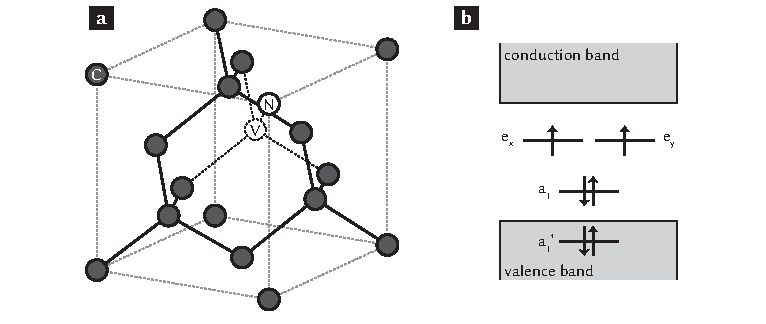
\includegraphics{figure_NV-structure-bernien}
	\caption{\label{fig:tam-fig1-nvstruct} \textbf{Crystal and electronic structure of the NV center} Figure from \cite{Bernien__2014}(a) The Nitrogen-Vacancy center defect is formed by a substitutional nitrogen atom (N) and a missing atom (vacancy, V) at an adjacant position in the diamond lattice (b) The electron occupation of the molecular orbitals in the electronic ground state, following Pauli's exclusion principle. The molecular orbitals are a linear combination of hybridised $sp^3$-orbitals. They are found by using the $C_{3v}$-symmetry of the NV center, taking into account the Coulomb interaction of the diamond nuclei and the lattice electrons with the electrons in the orbitals.}
\end{figure*}

In the electronic ground state, the 6 electrons occupy the molecular orbitals as shown in Fig. \ref{fig:tam-fig1-nvstruct}b. Excluding electron-electron interactions, the electronic ground-, ($^2a^2e$) and excited ($^1a^3e$) state are spin degenerate. This degeneracy is lifted by the Coulomb interaction between the electrons which leads to spin triplet (S = 1) ground-, and excited states ($^3A_2$ and $^3E$ respectively) as well as multiple intermediate spin singlet levels. The $^3A_2$ to $^3E$ transition energy of 1.945 eV lies in the optical regime (637 nm), well within the bandgap of diamond (5.5eV). Since all experimental techniques in this thesis aim to control the NV center in the spin triplet manifold, we will not discuss the singlet levels in further detail. For a more detailed discussion of the electronic structure of the NV-center we refer to a recent review of Doherty \textit{et al} \cite{Doherty_PhysicsReports_2013}.

\begin{figure*}
	\centering
	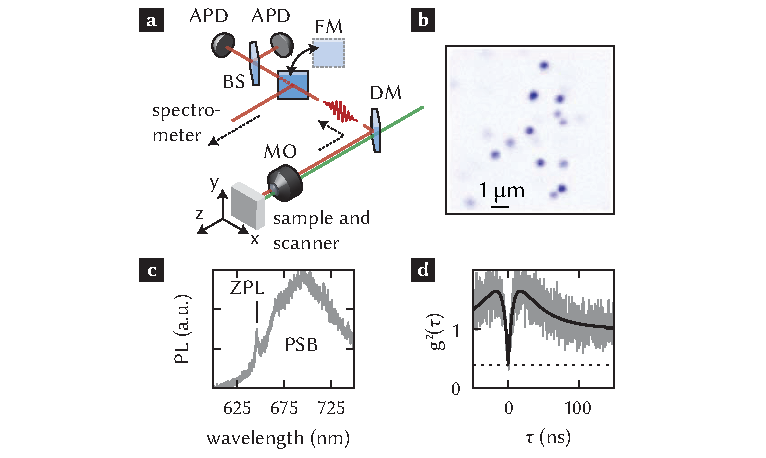
\includegraphics{figure_single_NVs-bernien}
	\caption{\label{fig:tam-fig2-nvstruct} \textbf{Detection of single NV centers} Figure from \cite{Bernien__2014}(a) Confocal microscope setup. The NV centers are excited by focussing a green (532 nm) excitation laser onto the sample using a microscope objective (MO). The sample is mounted on a piezo-stage allowing three-dimensional scans. The emission is spectrally filtered using a dicroic mirror (DM) and via a mechanically switchable mirror (FM) sent either to a spectrometer or to a beamsplitter (BS) followed by two APDs in a HBT-configuration. (b) Confocal scan of a bulk diamond sample. The intensity is plotted as a function of the stage position in \textit{x} and \textit{y}. Blue is higher intensity. (c) Emission spectrum of a single NV center with the zero phonon line at 637 nm and the phonon sideband at higher wavelengths. (d) Second-order autocorrelation function, with $\tau$ the delay between detection events of different detectors. The solid-line is a fit using a three-level model, including dark counts. The slow decay is associated with the decay from the singlet levels.}
\end{figure*}

We identify NV centers in bulk diamond at room-temperature in a home-build confocal microscope setup (Fig. \ref{fig:tam-fig2-nvstruct}a). By scanning the sample and collecting the fluorescence signal with a single photodiode (APD) we find multiple diffraction limited spots, corresponding to NV centers (Fig. \ref{fig:tam-fig2-nvstruct}b). Here we off-resonantly excite the NV center to a phonon level above the $^3E$ level, which quickly decays non-radiatively to $^3E$. The reflections of the excitation are separated from the fluorescence with a dicroic mirror. The emission spectrum from $^3E$ is show in Fig. \ref{fig:tam-fig2-nvstruct}c. It shows a distinct peak around 637 nm, corresponding to the direct decay from $^3E$ to $^3A_2$ (zero phonon line, ZPL) and a broad sideband corresponding to the decay to a phonon level above $^3A_2$ (phonon side band, PSB). To verify that the signal originates from a single emitter, we measure the second-order autocorrelation function $g^2 (\tau)$ in a Hanbury-Brown-Twiss configuration (Fig. \ref{fig:tam-fig2-nvstruct}d). The low probability of simultaneous photon detection ($g^2 (\tau = 0) < 1/2$) confirms that the signal comes from a single emitter.

\section{Single NV center device}

To enhance the collection and excitation efficiency of the NV center, a solid-immersion lens (SIL) is milled in the diamond using a focused ion beam (FIB) \cite{Hadden__2010,Marseglia__2011,Bernien__2014,Jamali__2014} (Fig. \ref{fig:tam-fig3-device}a). For an NV center in the middle of the SIL, the hemisphere ensures that the emission from the NV center reaches the diamond-air surface at normal incidence. This significantly reduces the loss due to total-internal reflection. For precise placement of the SIL, a pre-characterized NV center is located with respect to 1x1 $\mu$m gold markers that are fabricated on the surface of the diamond using electron beam lithography. The hemisphere structure is then created using a gallium ion beam by milling concentric rings of varying diameter around the position of the NV center. After milling the SILs, the sample is cleaned for 30 minutes in a boiling mixture of equal parts of perchloric, sulforic and nitric acid. This step removes the redeposited material during milling. A small conductive layer of gallium atoms that is implanted during the FIB process is removed by reactive-ion etching in an oxygen-plasma. 
\label{sec:devices}
\begin{figure*}
	\centering
	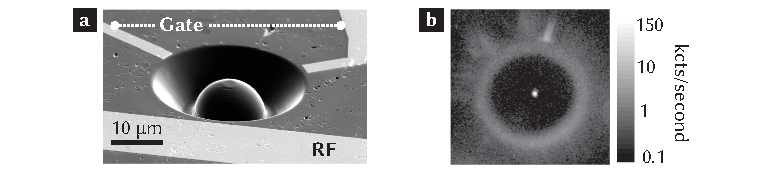
\includegraphics{figure_SIL_finished-bernien}
	\caption{\label{fig:tam-fig3-device} \textbf{} Figure from \cite{Bernien__2014} (a) }
\end{figure*}

A 200 nm thick gold microwave strip line for spin manipulation (Fig \ref{fig:tam-fig7-erabi} and \ref{fig:tam-fig10-nrabi}) and DC gates to DC stark shift the ZPL (see chapter \ref{ch:LDE}) are  fabricated near the SIL using electron beam lithography. Finally a single-layer anti-reflection coating\cite{Yeung__2012} (aluminium oxide) is fabricated on top of the sample to further increase the collection efficiency and reduce the reflection during resonant excitation (see chapter \ref{ch:LDE}).

\section{Addressing the electron excited state}
\label{sec:opticalcontrol}

The spin-orbit and spin-spin interactions introduce a fine splitting to the $^3E$ excited state which can be observed at cryogenic temperatures. The six resulting transitions have a distinct spin character (Fig. \ref{fig:tam-fig4-laserscan}a) and allow for spin-selective optical excitation of the electron. The transitions to the $m_s = 0$ states ($E_x$ and $E_y$) can occur upon absoprtion or emission of a linearly polarized photon, while the four $m_s = \pm 1$ transitions couple to circularly polarized light. The transition frequencies shift when an electric field or strain is applied. For an electric field along the N-V axis this results in an offset to the spectrum, not changing the energy level spacing. A perpendicular electric field affects the difference between the energy levels. As a result, the spectrum of the excited state slightly varies between NV centers due to local differences in strain and electric field. In Fig. \ref{fig:tam-fig4-laserscan}b we show measurements of the spectra of three different NV centres, normalized to have the same parallel strain. The lateral strain is determined from the difference between the transition energies of $E_x$ and $E_y$. The spectra show excellent agreement with the theoretical prediction (dashed lines). The strain typically differs a few tens of GHz between NV centers measured in this thesis.

\begin{figure*}
	\centering
	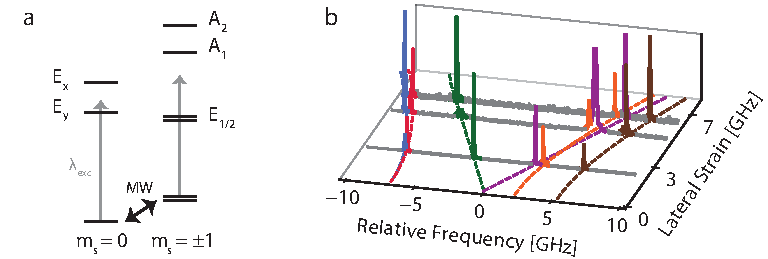
\includegraphics{laserscans}
	\caption{\label{fig:tam-fig4-laserscan} \textbf{Spectrum of the excited state} (a) Energy level diagram of the fine structure of the excited states. There are two levels with spin $m_s = 0$ ($E_x$,$E_y$) and four $m_s = \pm 1$ levels ($A_1$,$A_2$,$E_1$ and $E_2$). At finite strain the degeneracies between $E_x$,$E_y$ and $E_1$,$E_2$ are lifted. (b) The energy spectrum for three different NV centers is measured by varying the frequency of the excitation laser and detecting the fluorescence in the PSB. The observed transitions $E_1$ (blue), $E_2$ (red), $E_y$ (green), $E_x$ (purple), $A_1$ (orange) and $A_2$ (brown) are color coded and agree well with the theoretical prediction (colored dashed lines). For each scan the transition energies $\Delta E_x$ and $\Delta E_y$ are determined to calculate the lateral ($\frac{\Delta E_x-\Delta E_y}{2}$) and parallel ($\frac{\Delta E_y+\Delta E_x}{2}$) strain. The parallel strain is then substracted for each scan. Laser frequency is with respect to 470.4 THz.}
\end{figure*}

To address the spin-selective optical transitions in an experiment, we first verify that the NV center is in the $NV^-$ state and that the lasers are resonant with the desired transitions before each experimental run. During this charge-resonance (CR) check, we simultaneously apply two red lasers and monitor the fluorescence (Fig. \ref{fig:tam-fig4-cr}a). The lasers can only excite the electron spin for the NV center in $NV^-$ and the number of detected photons is highest when one red lasers is resonant with a $m_s = 0$ transition and the other with a $m_s=\pm1$ transition. We therefore compare the signal to a threshold and only continue with the experimental sequence when the threshold is passed (Fig. \ref{fig:tam-fig4-cr}b). When the number of detected photons is below the threshold we apply a green (523 nm) laser, perform another CR check and repeat until success. The green laser can repump the center to $NV^-$ by exciting trapped charges in the environment, but also induces spectral diffusion of the optical transitions since the local electric field is affected by the charge configuration in the environment. As an alternative to the green laser, a yellow laser ($\lambda \approx 575$ nm) can be used to resonantly excite the $NV^0$ zero phonon line \cite{Siyushev_Phys.Rev.Lett._2013}. 

\begin{figure*}
	\centering
	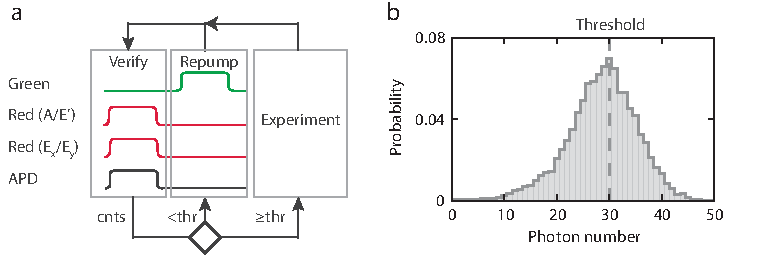
\includegraphics{CR}
	\caption{\label{fig:tam-fig4-cr} \textbf{Verifying the charge state and laser resonances} (a) Schematic of the experimental sequence to verify the charge state of the NV center and the laser resonances. The process is controlled by an ADwin microprocessor which turns on the two red lasers and compares the number of photons detected by the avalanche photodiode (APD) to a predetermined threshold (verify stage). When the number of detected photons is below the threshold a green laser is applied to prepare the $NV^-$ state (repump stage), otherwise the experimental sequence is initiated. (b) Photon number distribution during the verification stage, conditioned on the previous CR check being successful. }
\end{figure*}

The electron spin is initialized by selectively exciting a single transition\cite{Robledo_Nature_2011}: $E_x$ or $E_y$ to prepare $m_s = \pm 1$ or $A_1$/$A_2$/$E'$ to prepare $m_s=0$. The slight spin mixing of the excited states provides an optical pumping mechanism to prepare the opposite spin state (\ref{fig:tam-fig5-SP})a). The fluorescence observed during initialization (\ref{fig:tam-fig5-SP})b) exponentially decreases with the probability that the spin has flipped to a dark state that can not be excited by the pumping laser. The signal is fitted to an exponential decay to extract a lower bound for the preparation fidelity. To ensure that a pure state is prepared (as opposed to a mixture of $m_s = \pm 1$) the electron spin is typically initialized in $m_s = 0$, for this state we find a lower bound of $(99.7 \pm 0.1) \%$.

\begin{figure*}
	\centering
	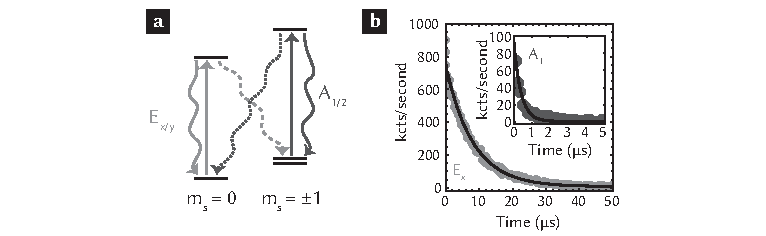
\includegraphics{figure_spinpumping-bernien}
	\caption{\label{fig:tam-fig5-SP} Figure from \cite{Bernien__2014} \textbf{Initialization by spin pumping} (a) Energy levels used to initialize (and readout) the electron spin. We excite transitions with a well-defined spin character of either $m_s = 0$ (bright arrows) or $m_s= \pm 1$ (dark arrows), resulting in spin-conserving optical cycling (indicated by bended solid arrows). Dashed arrows indicate the spin non-conserving decay paths. (b) Observed fluorescence when exciting $E_x$ ($A_1$) with the spin initially prepared in $m_s = \pm 1$ ($m_s = 0$). The signal is fitted to a single exponential with an offset to account for dark counts. From the fit we find a lower limit for the initialization fidelities: $(99.7 \pm 0.1) \%$ for $m_s = 0$ and $(99.2 \pm 0.1) \%$ for $m_s=\pm 1$.}
\end{figure*}

The observed fluorescence upon selective excitation provides a means to detect the electron spin state in a single shot\cite{Robledo_Nature_2011}. To characterize the readout we plot the distribution of photons detected in the PSB collected during a 10 $\mu s$ laser pulse exciting $E_x$ (fig \ref{fig:tam-fig6-ssro}a). The distributions are clearly separated depending on the initial spin state, allowing us to assign $m_s = 0$ to the cases where one or more photons are detected and $m_s = \pm 1$ otherwise. The combined readout and initialization fidelity for $m_s = \pm 1$ ($F_1 = .989 \pm .001$) is reduced by detector dark counts and off-resonant excitation, while for $m_s = 0$ ($F_1 = .956 \pm .003$) the error is governed by the instances where the spin is flipped before a photon is detected. This can be seen in fig \ref{fig:tam-fig6-ssro}b where the readout fidelities are plotted as a function of readout duration. The fidelity for $m_s = 0$ initially increases with readout time and then saturates indicating that the spin has flipped with high probability. The optimal mean readout fidelity ($F_{ro} = \frac{F_0+F_1}{2} = 0.973 \pm 0.002$) is reached after $10 \mu s$.

\begin{figure*}
	\centering
	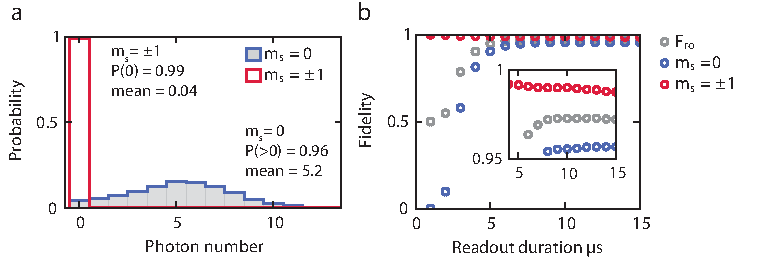
\includegraphics{ssro}
	\caption{\label{fig:tam-fig6-ssro} \textbf{Single shot readout} (a) Histograms of the number of detected photons in the PSB for initial state $m_s = 0$ (blue) and $m_s=\pm 1$ (red) during a 10 $\mu s$ readout on $E_x$. (b) Fidelities for reading out the electron spin state initially prepared in $m_s = 0$ (blue) and $m_s = \pm 1$ (red) as a function of readout duration. The mean readout fidelity is plotted in grey. The inset is a zoom of the region where the optimal mean readout fidelity is reached.}
\end{figure*}

\section{Ground state spin control and coherence}

In the orbital ground state, the $m_s = 0$ and $m_s = \pm 1$ states are separated by the zero-field splitting $D \approx 2.88$ GHz, while an external magnetic field lifts the degeneracy between $m_s = +1$ and $-1$ via the zeeman splitting. The hamiltonian is given by

\begin{equation}
H_{GS} = D^2 S_z + \gamma_e \mathbf{B} \cdot \mathbf{S}
\end{equation}

with $\mathbf{S} =[S_x,S_y,S_z]$,  $S_i$ the pauli spin matrices for a spin-1 particle and $\gamma_e = 2.8$ MHz/G the gyromagnetic ratio of the electron. We define our qubit in the $m_s = 0 :\ket{0}$ and $m_s = -1 : \ket{1}$ states (alternatively the $m_s = + 1$ state can be used to encode $\ket{1}$). The electron spin is manipulated with electron spin resonance techniques by sending an ac current through the stripline generating an oscillating magnetic field at the location of the NV center. At the resonance condition the frequency of the control field matches the energy difference between the $\ket{0}$ and $\ket{1}$ states resulting in coherent Rabi oscillations between those levels as shown in fig \ref{fig:tam-fig7-erabi}. Arbitrary qubit rotations are implemented by calibrating the amplitude (which sets the rabi frequency) and length of the control pulses.


Spin manipulation with ESR techniques. (Fig. \ref{fig:tam-fig7-erabi})

Figure to add: Coherence times $T_2^{*}$, $T_2$ and dynamical decoupling.

\label{sec:groundstatecontrol}
\begin{figure*}
	\centering
	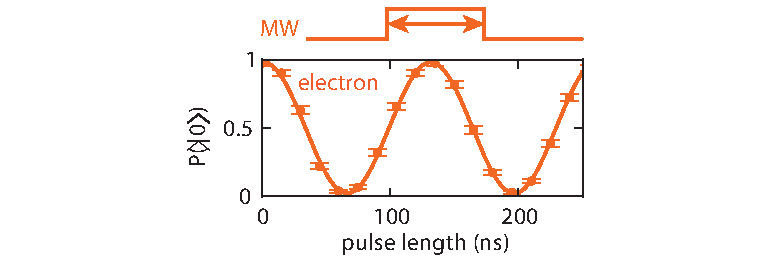
\includegraphics{electron_rabi}
	\caption{\label{fig:tam-fig7-erabi} \textbf{} (a) Coherent qubit rotations of the electron spin are performed by varying the length of a MW pulse. The signal is corrected to account for imperfect readout and initialization. Solid line is a sinusoidal fit from which we determine the Rabi frequency $(7.67 \pm 0.02)$ MHz}
\end{figure*}

%\begin{figure*}
%	\centering
%	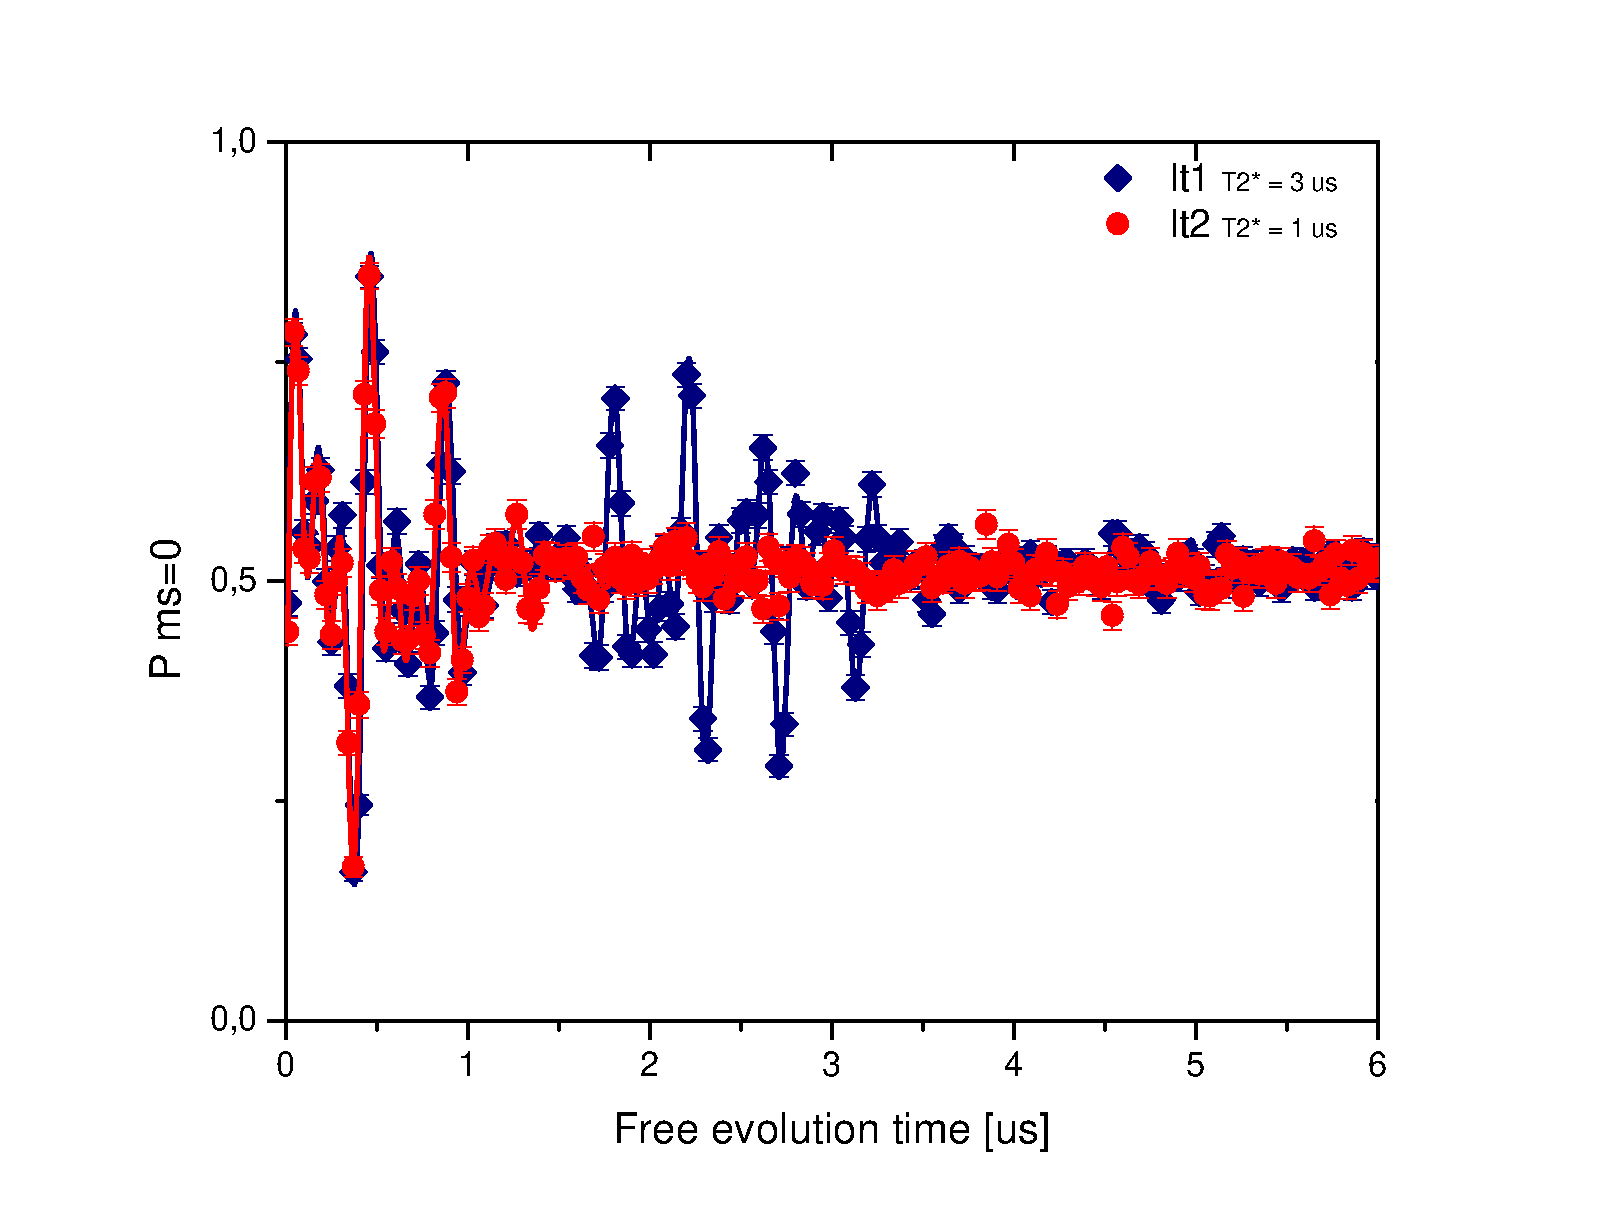
\includegraphics{ramsey-LDE}
%	\caption{\label{fig:tam-fig8-eramsey} \textbf{} (a) }
%\end{figure*}

\begin{figure*}
	\centering
	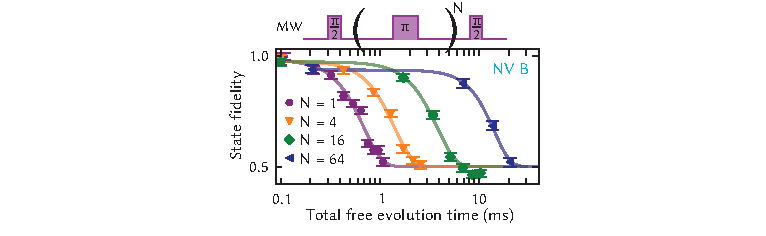
\includegraphics{DD-LDE_bernien}
	\caption{\label{fig:tam-fig9-DD} \textbf{Dynamical Decoupling of the electron spin} (a) }
\end{figure*}

\section{Coupling to nuclear spins}

Hyperfine coupling to nitrogen spin and NMR.

Figure to add: ESR with visible splitting of the $^{14}N$ spin and nuclear rabi
%\label{sec:nuclearspins}
%\begin{figure*}
%	\centering
%	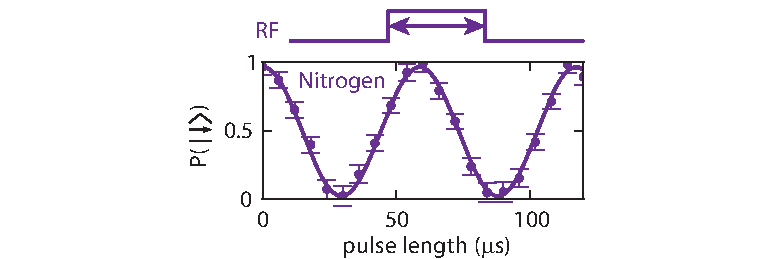
\includegraphics{nitrogen_rabi}
%	\caption{\label{fig:tam-fig10-nrabi} \textbf{} (a) }
%\end{figure*}
%\section{Quantum measurements}


%\section{Methods}



\newpage
\bibliographystyle{../thesis}
\bibliography{tam}




\graphicspath{{./ch_adptv_msmnt_cntrl/figures/}}


\chapter[Manipulating a qubit through the backaction of adaptive measurements]{Manipulating a qubit through the backaction of sequential partial measurements \\ and real-time feedback }
\label{ch:AMC}

\begin{center} 
    \vspace{-1cm} {M.S.~Blok$^*$, C.~Bonato$^*$, M.L.~Markham, D.J. ~Twitchen, V.V. ~Dobrovitski and R.~Hanson} 
\end{center}


{\renewcommand{\thefootnote}{}\footnote{This chapter has been published in
    {\em Nature Physics} \textbf{10}, 189-193 (2014).}\footnote{$^*$ these authors contributed equally to this work}}


\vspace{-0.5cm} 
Quantum measurements not only extract information from a system but also alter its state. Although the outcome of the measurement is probabilistic, the backaction imparted on the measured system is accurately described by quantum theory ~\cite{Guerlin_Nature_2007,Hatridge_Science_2013,Murch_Nature_2013}. Therefore, quantum measurements can be exploited for manipulating quantum systems without the need for control fields~\cite{Ashhab_PhysRevA_2010,Wiseman_NatureNV_2011}. We demonstrate measurement-only state manipulation on a nuclear spin qubit in diamond by adaptive partial measurements. We implement the partial measurement via tunable correlation with an electron ancilla qubit and subsequent ancilla readout~\cite{Brun_PhysRevA_2008,Groen_PRL_2013}. We vary the measurement strength to observe controlled wavefunction collapse and find post-selected quantum weak values~\cite{Brun_PhysRevA_2008,Groen_PRL_2013,Aharonov_PRL_1988,Pryde_PRL_2005,Dressel_ArXiv_2013}. By combining a novel quantum non-demolition readout on the ancilla with real-time adaption of the measurement strength we realize steering of the nuclear spin to a target state by measurements alone. Besides being of fundamental interest, adaptive measurements can improve metrology applications~\cite{Cappellaro_PhysRevA_2012,Higgins_Nature_2007} and are key to measurement-based quantum computing~\cite{Raussendorf_PRL_2001,Prevedel_Nature_2007}.


\clearpage

\section{Introduction}
Measurements play a unique role in quantum mechanics and in quantum information processing. The backaction of a measurement can be used for state initialization~\cite{Robledo_Nature_2011,Riste_PRL_2012}, generation of entanglement between non-interacting systems~\cite{Chou_Nature_2005,Moehring_Nature_2007,Pfaff_NatPhys_2012,Riste_Nature_2013}, and for qubit error detection~\cite{Chiaverini_Nature_2004}. These measurement-based applications require either post-selection or real-time feedback, as the outcome of a measurement is inherently probabilistic. Recent experiments achieved quantum feedback control on a single quantum system~\cite{Riste_Nature_2013, Gillett_PRL_2010,Sayrin_Nature_2011,Vijay_Nature_2012} by performing coherent control operations conditioned on a measurement outcome.

Here, we realize real-time adaptive measurements and exploit these in a proof-of-principle demonstration of measurement-only quantum feedback. Our protocol makes use of partial measurements that balance the information gain and the measurement backaction by varying the measurement strength. We accurately control the measurement strength and the corresponding backaction in a two-qubit system by tuning the amount of (quantum) correlation between the system qubit and an ancilla qubit, followed by projective readout of the ancilla~\cite{Brun_PhysRevA_2008,Groen_PRL_2013}. In general, the backaction of sequential partial measurements leads to a random walk~\cite{Guerlin_Nature_2007,Hatridge_Science_2013,Murch_Nature_2013} but by incorporating feedback, multiple measurements can direct the trajectory of a qubit towards a desired state~\cite{Ashhab_PhysRevA_2010,Wiseman_NatureNV_2011}. Real-time adaptive measurements are a key ingredient for quantum protocols such as one-way quantum computing~\cite{Raussendorf_PRL_2001,Prevedel_Nature_2007} and Heisenberg-limited phase estimation~\cite{Cappellaro_PhysRevA_2012,Higgins_Nature_2007}.

We implement the adaptive partial measurements in a nitrogen vacancy (NV) center in synthetic diamond. We define the system qubit by the nuclear spin of the NV host nitrogen ($\ket{\downarrow}$: $m_I$=0, $\ket{\uparrow}$: $m_I$= -1), and the ancilla qubit by the NV electron spin ($\ket{0}$: $m_S$=0, $\ket{1}$: $m_S$=-1) (Fig.\,\ref{fig:amc-fig1}a). The ancilla is initialized and read out in a single shot with high fidelity using spin-selective optical transitions~\cite{Robledo_Nature_2011}. We perform single-qubit operations on the ancilla by applying microwave frequency pulses to an on-chip stripline.


\section{Variable-strength measurement}
\begin{figure*}
	\centering
	\includegraphics{fig1_twocolumns}
	\caption{\label{fig:amc-fig1} \textbf{Partial measurement of a spin qubit in diamond.} (a) The NV center is a natural two-qubit system where the system qubit is defined by the $^{14}N$ nuclear spin and the ancilla qubit is defined by the electron spin. A solid-immersion-lens is deterministically fabricated on top of the selected NV center to increase the photon collection efficiency. Control fields for single qubit rotations are generated by applying a current to the gold stripline (yellow).  (b) A tunable strength measurement is implemented by a Ramsey-type gate on the ancilla. We plot the probability to measure the state $\ket{0}$  for the ancilla, as a function of interaction time $\tau$, for two system input states $\ket{\downarrow}$ (red) and $\ket{\uparrow}$ (blue). The Bloch-spheres show the state of the system (purple) and ancilla (orange) after the entangling-gate for the different input states (red and blue vectors). The colour bar represents the measurement strength, proportional to $\sin{\theta}$, where $\theta=\frac{A \tau}{2}$. Blue corresponds to a projective measurement and white to no measurement. Solid lines are a  fit to the function $y_0 + e^{-( \frac{\tau}{T_2^*})^2} \cos{(A \tau + \delta)} $. From the phase offset $\delta$ we find the weakest measurement we can perform, corresponding to $\theta = 5^{\circ}$. This is limited by free evolution of the ancilla during the pulses.(see Methods). Error bars depict 68 $\%$ confidence intervals. Sample size is 500 for each data point. }
\end{figure*}

We realize the variable-strength measurement by correlating the system qubit with the ancilla through a controlled-phase-type gate (Fig.\,\ref{fig:amc-fig1}b) that exploits the hyperfine interaction, which (neglecting small off-diagonal terms) has the form $\hat{H}_{hf}=A\hat{S}_{z}\hat{I}_{z}$ (with $A = 2 \pi \times 2.184 \pm 0.002$ MHz and $\hat{S}_{z}, \hat{I}_{z}$ the three-level Pauli z-operators for the electron, nuclear spin respectively).  During free evolution, the ancilla qubit precession is conditional on the state of the system qubit. We choose the rotating frame such that the ancilla rotates clockwise (anti-clockwise) around the z-axis if the system qubit is in $\ket{\uparrow}$ ($\ket{\downarrow}$) and vary the interaction time $\tau$. For $\tau = 0$, there is no correlation between the ancilla and the system, whereas for $\tau = \frac{\pi}{A}$, corresponding to the rotation angle $\theta = 90^{\circ}$, the two are maximally correlated. A subsequent rotation and projective readout of the ancilla then implements a measurement of the system qubit, with a measurement strength that can be accurately tuned by controlling the interaction time $\tau$. A mathematical derivation  can be found in the methods.

We investigate the measurement-induced backaction by preparing an initial state of the system ($\ket{\up},\ket{x}$ and $\ket{y}$) and performing a partial measurement with strength $\theta$, followed by state tomography (Fig.\,\ref{fig:amc-fig2}a). First, we neglect the outcome of the partial measurement, which is mathematically equivalent to taking the trace over the state of the ancilla qubit. In this case the backaction is equivalent to pure dephasing as can be seen by a measured reduction of the length of the Bloch vector (Fig.\,\ref{fig:amc-fig2}b). Next, we condition the tomography on the ancilla measurement yielding state $\ket{0}$ (Fig.\,\ref{fig:amc-fig2}c). We observe that for a weak measurement $(\theta = 5^{\circ})$, the system is almost unaffected, whereas for increasing measurement strength it receives a stronger kick towards $\ket{\uparrow} $(Fig.\,\ref{fig:amc-fig2}c). Crucially, we find that the length of the Bloch vector is preserved in this process, as expected for an initially pure state. This shows that the partial collapse is equivalent to a qubit rotation that is conditional on the measurement strength and outcome and on the initial state. By performing quantum process tomography, we find that both measurement processes agree well with the theoretical prediction (the process fidelities are 0.986 $\pm$ 0.004 and 0.94 $\pm$ 0.01 for the unconditional and conditional process, respectively; see Methods).


\begin{figure}
	\centering
	\includegraphics{fig2_partial_measurement_backaction}
	\caption{\label{fig:amc-fig2} \textbf{Measurement backaction for variable-strength measurement}. (a) We prepare an initial state  of the system ($\ket{\uparrow}$,  $\ket{x}$ and  $\ket{y}$), perform a partial measurement with strength $\theta$, and characterize the measurement backaction on the system by quantum state tomography. Quantum state tomography is implemented by an ancilla-assisted projective measurement, performed with the same protocol, setting $\tau = 229$ ns for $\theta = 90^{\circ}$. The nuclear spin basis rotation is performed with a $\frac{\pi}{2}$ radio-frequency pulse (along either $x$ or $y$). The basis rotation pulse for the tomography is applied before the readout of the ancilla, to avoid the dephasing induced by the state-characterization measurement (see main text). The data is corrected for errors in the readout and initialization of the system qubit, both of which are obtained from independent measurements (see methods). (b,c)  Measurement backaction for a partial measurement of increasing strength, independent of the measurement result for the ancilla qubit (b), or conditioned on the ancilla in  $\ket{0}$ (c). }
\end{figure}

\section{Generalized weak value}
By combining a partial measurement with post-selection on the outcome of a subsequent projective measurement, we can measure the generalized weak value $_{f} \langle I_{z} \rangle$ (conditioned average of contextual values \cite{Dressel_PRL_2010}, see methods) of the nuclear spin in the $z$-basis. In the limit of zero measurement strength ($\theta = 0^{\circ}$), this quantity approximates the weak value \cite{Aharonov_PRL_1988} $W = \frac{\bra{\psi_f} \hat{I}_z \ket{\psi_i}}{\bra{\psi_f} \psi_i \rangle}$ , where $ \psi_i (\psi_f )$ is the initial (final) state of the nucleus and from here we define $\hat{I}_z$ as the Pauli $z$-operator reduced to a two-level system with eigenvalues +1 and $-$1. By post-selecting only on the final states having small overlap with the initial state, $_{f} \langle I_{z} \rangle$ can be greatly amplified to values that lie outside the range of eigenvalues of the measured observable. As shown in Fig.\,\ref{fig:amc-fig3}, by sweeping the angle between the initial and final states we observe up to tenfold amplification ($_{f} \langle I_{z} \rangle = 10 \pm 3$) compared to the maximum eigenvalue of $I_{z}$ ($+1$). This amplification is the highest reported for a solid-state system to date\cite{Groen_PRL_2013}. As predicted \cite{Williams_PRL_2008}, we observe that values of  $_{f} \langle I_{z} \rangle$ lying outside of the range of eigenvalues of $I_{z}$ can be found for any finite measurement strength.

\begin{figure}
	\centering
	\includegraphics{fig3_weak_value}
	\caption{\label{fig:amc-fig3} \textbf{Generalized quantum weak value}. Measurement of a generalized weak value for the nuclear-spin qubit, performed by a partial measurement of strength $\theta$, followed by a strong measurement and post-selection of the state  $\ket{\downarrow}$, as a function of the basis rotation angle $\phi$ of the strong measurement (Fig.\,\ref{fig:amc-fig2}a). Solid lines are simulations using independently determined parameters. The asymmetry in the curve can be explained by asymmetric nuclear spin flips arising during ancilla initialisation by optical excitation of the forbidden transition of $E_{y}$ (see methods). Inset: the generalized weak values as a function of the strength $\theta$ of the partial measurement, setting the basis rotation angle of the strong measurement to the optimal value  $\phi = \frac{\pi}{2} - \theta$. All error bars depict 68 $\%$ confidence intervals. The sample size varies per data point because each data point has different post-selection criterion.}
\end{figure}

\section{QND-measurement of the ancilla qubit}
Using the partial measurements for measurement-based feedback requires reading out the ancilla without perturbing the system qubit. In our experiment the system qubit can dephase during ancilla readout both through a spin-flip of the electron in the course of optical excitation (Fig.\,\ref{fig:amc-fig4}b) and as a result of the difference in the effective nuclear g-factor in the electronic ground- and optically excited state~\cite{Jiang_PRL_2008}. Note that for the characterization of a single partial measurement (Fig.\,\ref{fig:amc-fig2}) we circumvent this dephasing by interchanging the measurement basis rotation and the ancilla readout; this interchange is not possible for real-time adaptive measurements.

\begin{figure*}
	\centering
	\includegraphics{fig4_qnd_electron}
	\caption{\label{fig:amc-fig4} \textbf{Quantum non-demolition measurement of the ancilla qubit} (a) The ancilla is initialized in $\ket{0}$ ($\ket{1}$) by optically pumping the $A_2$ ($E_y$) transition. The ancilla is then read out by exciting the $E_y$ transition for 100 $\mu$s (conventional readout), or until a photon was detected (dynamical-stop readout). Finally, we verify the post-measurement state with a conventional readout. (b) Fidelity of the post-measurement state of the ancilla for conventional readout (left graph) and dynamical-stop readout (right graph). Results are corrected for the infidelity in the final readout.  All error bars depict 68 $\%$ confidence intervals. Sample size per datapoint is 5000 }
\end{figure*}

To mitigate the nuclear dephasing during ancilla readout we reduce the ancilla spin-flip probability using a dynamical-stop readout technique. We partition the optical excitation time in short ($1~ \mu$s) intervals and we stop the excitation laser as soon as a photon is detected, or after a predetermined maximum readout time when no photon is detected (Fig.\,\ref{fig:amc-fig4}a). This reduces redundant excitations without compromising the readout fidelity. In Fig.\,\ref{fig:amc-fig4}b we show the correspondence between pre- and post-measurement states for the two eigenstates of the ancilla. For the state $\ket{0}$ the dynamical-stop readout increases the fidelity ($F = \bra{\psi_i}\rho_m \ket{\psi_i}$, where $\rho_m$ is the density matrix of the system after the ancilla readout) from 0.18 $\pm$ 0.02 to 0.86 $\pm$ 0.02. The latter fidelity is solely limited by the cases where the spin flipped before a photon was detected: we find $F = 1.00 \pm 0.02$ for the cases in which a photon was detected. As expected, the fidelity is high ($F = 0.996 \pm 0.006$) for input state $\ket{1}$ as this state is unaffected by the excitation laser. The dynamical-stop technique thus implements a quantum non-demolition (QND) measurement of the ancilla electron spin with an average fidelity of 0.93 $\pm$ 0.01 for the post-measurement state.

The dynamical-stop readout of the ancilla significantly reduces the dephasing of the nuclear spin qubit during measurement as shown in Fig.\,\ref{fig:amc-fig5}. Starting with the nuclear spin in state $\ket{x} = \frac{\ket{0} + \ket{1}}{\sqrt{2}}$, a conventional readout of the ancilla completely dephases the nuclear spin, leading to a state fidelity with respect to $\ket{x}$ of 0.5. In contrast, the fidelity of the dynamical-stop readout saturates to 0.615 $\pm$ 0.002 (probably limited by changes in the effective g-factor of the nuclear spin). The dynamical-stop readout thus leaves the system in a coherent post-measurement state that can be used in a real-time feedback protocol. 

\begin{figure*}
	\centering
	\includegraphics{fig5_qnd_nuclear_spin}
	\caption{\label{fig:amc-fig5} \textbf{System qubit coherence during ancilla readout}. Coherence of the system qubit state after ancilla readout. For the dynamical-stop protocol we define the ancilla readout time as the predetermined maximum readout time. The graph shows the fidelity of the system with respect to $\ket{x}$ for conventional readout (red) and dynamical-stop readout (blue). The $z$-component of the system is unaffected as shown by the constant fidelity with respect to $\ket{\uparrow}$ (grey). All error bars depict 68 $\%$ confidence intervals. Sample size per datapoint is 2000 }
\end{figure*}

\section{Control by adaptive measurements}
Preserving coherence of the post-measurement state enables a proof-of-principle realization of measurement-only control, by implementing sequential measurements and tuning the strength of the second measurement in real time conditioned on the outcome of the first measurement (Fig.\,\ref{fig:amc-fig6}a). We choose as our target the creation of the state $\ket{\psi} = \cos{(\frac{\pi}{4}+\frac{\theta_1}{2})}\ket{\downarrow}+\cos{(\frac{\pi}{4}-\frac{\theta_1}{2})}\ket{\uparrow}$ from initial state $\ket{x}$ using only partial measurements of $\hat{I}_z$. The first measurement with strength $\theta_1$ will prepare either the desired state, or the state $\ket{\psi_{wrong}} =  \cos{(\frac{\pi}{4}-\frac{\theta_1}{2})}\ket{\downarrow}+\cos{(\frac{\pi}{4}+\frac{\theta_1}{2})}\ket{\uparrow}$ , each with probability 0.5. We adapt the strength of the second measurement $\theta_2$ according to the outcome of the first measurement: we set $\theta_2 = 0$ if the first measurement directly yielded the target state, but if the wrong outcome was obtained we set the measurement strength to

\begin{equation}
\theta_2 = \sin{^{-1}\left[2 \frac{\sin{\theta_1}}{1 + \sin{^2 \theta_1}}\right]},
\end{equation}

such that the second measurement will probabilistically rotate the qubit to the target state (see methods). The total success probability of this two-step protocol is  $p_{suc} = \frac{1}{2}(1 + \cos{\theta_1})$ and a successful event is heralded by the outcome of the ancilla readout. In principle the protocol can be made fully deterministic~\cite{Ashhab_PhysRevA_2010} by incorporating a reset in the form of a projective measurement along the $x$-axis.

To find the improvement achieved by the feedback, we first compare the success probability of our adaptive measurement protocol to the success probability for a single measurement (Fig.\,\ref{fig:amc-fig6}b right panel). The success probability clearly increases with the adaptive protocol and is proportional to the readout fidelity of the $\ket{0}$ state of the ancilla, which is maximum for readout times  \textgreater~25~$\mu$s. The fidelity of the final state (Fig.\,\ref{fig:amc-fig6}b left panel) is limited by the remaining dephasing of the system during readout of the ancilla as shown in Fig.\,\ref{fig:amc-fig5}. This constitutes the trade-off between success probability and state fidelity. 

We show that the increase in success probability is enabled by feedback by comparing the final state fidelity with and without feedback (Fig.\,\ref{fig:amc-fig6}b left panel). In principle the success probability can be increased in the absence of feedback by accepting a certain number of false measurement outcomes at the cost of a reduced fidelity. We calculate the maximum fidelity that can be achieved in this way by performing only the first measurement and increasing the success probability to that of the adaptive protocol using post-selection (grey line in Fig.\,\ref{fig:amc-fig6}b, left panel). We find that the measured state fidelity in the adaptive protocol is above this bound (Fig.\,\ref{fig:amc-fig6}b, green area), which indicates that the adaptive measurement indeed successfully corrects the kickback from the first measurement, thus yielding a clear advantage over open-loop protocols.



We note that, in contrast to pioneering adaptive measurement experiments on photons that only used experimental runs in which a photon was detected at each measurement stage~\cite{Prevedel_Nature_2007}, our protocol is fully deterministic in the sense that the partial measurement always yields an answer. In particular, the data in Fig.\,\ref{fig:amc-fig6} includes all experimental runs and thus no post-selection is performed, as desired for future applications in metrology and quantum computing. 

The performance of the protocol can be further improved by increasing the ancilla readout fidelity (either by improving the collection efficiency or reducing spin-flip probability) and by further reducing the dephasing of the system during readout. A particularly promising route is to use nuclear spins farther away from the NV center (for example carbon-13 spins) that have much smaller hyperfine couplings~\cite{Zhao_NatureNano_2012,Taminiau_PRL_2012,Kolkowitz_PRL_2012} and are more robust against changes in the orbital state of the electron spin.

\begin{figure*}
	\centering
	\includegraphics{fig6_adaptive_protocol}
	\caption{\label{fig:amc-fig6} \textbf{Manipulation of a nuclear spin state by sequential partial adaptive measurements with real-time feedback.} (a) Adaptive measurement protocol. The ancilla qubit is initialized in $\ket{0}$ and the system qubit is prepared in $\ket{x}$. The strength of the second measurement ($\theta_2$) is adjusted according to the outcome of the first measurement. The system is analysed by state tomography at each intermediate step. The result of the tomography is plotted on the bloch spheres (blue vector) and compared with the ideal case (grey vector). (b) Fidelity of the output state with respect to the target state as a function of ancilla readout time (dynamical-stop readout) with feedback (only the cases where the protocol heralds success). The grey line is obtained by performing one measurement and adding negative results to artificially increase the success probability to that of the adaptive protocol (red line in right panel). In the right panel we show the probability that the protocol heralds success for one measurement and for the adaptive protocol.  }
\end{figure*}

Our work is the first experimental exploration of a fundamental concept of control-free control \cite{Jordan_PRB_2006, Ashhab_PhysRevA_2010, Wiseman_NatureNV_2011} . Furthermore, the use of adaptive measurements as presented here can increase the performance of spin-based magnetometers \cite{Cappellaro_PhysRevA_2012, Higgins_Nature_2007}. Finally, our results can be combined with recently demonstrated methods for generating entanglement between separate nitrogen vacancy centre spins \cite{Bernien_Nature_2013, Dolde_NatPhys_2013}. Taken together, these techniques form the core capability required for one-way quantum computing, where quantum algorithms are executed by sequential adaptive measurements on a large entangled 'cluster' state \cite{Raussendorf_PRL_2001, Prevedel_Nature_2007}.

%In conclusion, we implemented sequential partial measurements and showed that by adjusting the measurement strength in real-time we can steer a quantum system towards a desired state. Our work is the first experimental exploration of a fundamental concept in the field of quantum measurement and control~\cite{Wiseman_NatureNV_2011} that may find application in systems where control fields are difficult to generate. Furthermore, the use of adaptive measurements as presented here can increase the performance of spin-based magnetometers~\cite{Cappellaro_PhysRevA_2012,Higgins_Nature_2007}. Finally, our results can be combined with recently demonstrated methods for generating entanglement between separate NV center spins~\cite{Bernien_Nature_2013,Dolde_NatPhys_2013}. Taken together, these techniques form the core capability required for one-way quantum computing, where quantum algorithms are executed by sequential adaptive measurements on a large entangled ‘cluster’ state~\cite{Raussendorf_PRL_2001,Prevedel_Nature_2007}.
\section{Methods}
We use a naturally-occurring nitrogen-vacancy center in high-purity type IIa CVD diamond, with a \textless 111\textgreater-crystal orientation obtained by cleaving and polishing a \textless100\textgreater -substrate. Experiments are performed in a bath cryostat, at the temperature of 4.2 K, with an applied magnetic field of 17 G. Working at low-temperature, we can perform efficient electron spin initialization (F = 0.983 $\pm$ 0.006) and single-shot readout (the fidelity is 0.853 $\pm$ 0.005 for $m_S = 0$ and 0.986 $\pm$ 0.002 for $m_S = -1$) by spin-resolved optical excitation~\cite{Robledo_Nature_2011}. Initialization of the nuclear spin is done by measurement~\cite{Robledo_Nature_2011}, with fidelity  0.95~$\pm$~0.02. Single-qubit operations can be performed with high accuracy using microwave (for the electron) and radio-frequency (for the nucleus) pulses applied to the gold stripline. Note that the single-qubit operations on the nucleus are only used for state preparation and tomography, but not in the feedback protocol. The dephasing time $T_2^*$ is (7.8~$\pm$~0.2)~ms for the nuclear spin and (1.35~$\pm$~0.03)~$\mu$s for the electron spin. 
\newpage
\bibliographystyle{../thesis}
\bibliography{amc}





\graphicspath{{./ch_adptv_msmnt_magnetometry/figures/}}


\chapter[Optimized quantum sensing using real-time adaptive measurements]{ Optimized quantum sensing with a single electron spin using real-time adaptive measurements}
\label{ch:AMM}

\begin{center} 
    \vspace{-1cm} {C.~Bonato$^*$, M.S.~Blok$^*$, H.T. ~Dinani, D.W. ~Berry, M.L. ~Markham, D.J. ~Twitchen  and R.~Hanson} 
\end{center}

{\renewcommand{\thefootnote}{}\footnote{This chapter has been submitted to
    {\em Nature Nanotechnology} (2015).}\footnote{$^*$ these authors contributed equally to this work}}

\vspace{-0.5cm} 
Quantum sensors based on single solid-state spins promise a unique combination of sensitivity and spatial resolution ~\cite{Giovannetti_NatPhoton_2011,Higgins_Nature_2007,Degen_APL_2008,Taylor_NatPhys_2008,Maze_Nature_2008,Balasubramanian_Nature_2008,Balasubramanian_NatMater_2009,Dolde_NatPhys_2011,Acosta_Phys.Rev.Lett._2010,Toyli_PNAS_2013,Ovartchaiyapong_NatCommun_2014,LeSage_Nature_2013,Kaufmann_PNAS_2013,Kucsko_Nature_2013,Shi_Science_2015,Maletinsky_NatNano_2012,Staudacher_Science_2013,Mamin_Science_2013,Tetienne_Science_2014,Kolkowitz_Science_2015}. The key challenge in sensing is to achieve minimum estimation uncertainty within a given time and with a high dynamic range. Adaptive strategies have been proposed to achieve optimal performance but their implementation in solid-state systems has been hindered by the demanding experimental requirements. Here we realize adaptive d.c. sensing by combining single-shot readout of an electron spin in diamond with fast feedback. By adapting the spin readout basis in real time based on previous outcomes we demonstrate a sensitivity in Ramsey interferometry surpassing the standard measurement limit. Furthermore, we find by simulations and experiments that adaptive protocols offer a distinctive advantage over the best-known non-adaptive protocols when overhead and limited estimation time are taken into account. Using an optimized adaptive protocol we achieve a magnetic field sensitivity of $6.1\pm 1.7$ nT Hz$^{-\frac{1}{2}}$ over a wide range of 1.78 mT. These results open up a new class of experiments for solid-state sensors in which real-time knowledge of the measurement history is exploited to obtain optimal performance.


\clearpage

\section{Introduction}
Quantum sensors have the potential to achieve unprecedented sensitivity by exploiting control over individual quantum systems\cite{Giovannetti_NatPhoton_2011,Higgins_Nature_2007}. As a prominent example, sensors based on single electron spins associated with Nitrogen-Vacancy (NV) centers in diamond capitalize on the spin's quantum coherence and the high spatial resolution resulting from the atomic-like electronic wave function \cite{Degen_APL_2008,Taylor_NatPhys_2008}. Pioneering experiments have already demonstrated single-spin sensing of magnetic fields\cite{Maze_Nature_2008,Balasubramanian_Nature_2008,Balasubramanian_NatMater_2009}, electric fields \cite{Dolde_NatPhys_2011}, temperatures\cite{Acosta_Phys.Rev.Lett._2010,Toyli_PNAS_2013} and strain\cite{Ovartchaiyapong_NatCommun_2014}. NV sensors may therefore have a revolutionary impact on biology\cite{LeSage_Nature_2013,Kaufmann_PNAS_2013,Kucsko_Nature_2013,Shi_Science_2015}, nanotechnology\cite{Maletinsky_NatNano_2012,Staudacher_Science_2013,Mamin_Science_2013} and material science\cite{Tetienne_Science_2014,Kolkowitz_Science_2015}. 

\section{D.C. Magnetometry}
A spin-based magnetometer can sense a d.c. magnetic field \textit{B} through the Zeeman shift $E_z=\hbar \gamma B = \hbar 2 \pi f_B$ ($\gamma$ is the gyromagnetic ratio and $f_B$ the Larmor frequency) between two spin levels $\ket{0}$ and $\ket{1}$. In a Ramsey interferometry experiment, a superposition state  $\frac{1}{\sqrt{2}}$($\ket{0}$ + $\ket{1}$), prepared by a $\pi$/2 pulse, will evolve to $\frac{1}{\sqrt{2}}$($\ket{0}$ + $e^{i\varphi}\ket{1}$)   over a sensing time \textit{t}. The phase $\varphi = 2 \pi f_B t$ can be measured by reading out the spin in a suitable basis, by adjusting the phase $\vartheta$ of a second $\pi$/2 pulse.


For a Ramsey experiment that is repeated with constant sensing time \textit{t} the uncertainty $\sigma_{f_B}$ decreases with the total sensing time \textit{T} as 1/(2 $\pi \sqrt{tT}$) (standard measurement sensitivity, SMS).  However, the field range also decreases with \textit{t} because the signal is periodic, creating ambiguity whenever $|2\pi f_B t| > \pi $. This results in a dynamic range bounded as  $f_{B,max}$/$\sigma_{f_B}  \le \pi \sqrt{T/t}$.  Recently, it was discovered that the use of multiple sensing times within an estimation sequence can yield a scaling of $\sigma_{f_B}$ as 1/\textit{T}, resulting in a vastly improved dynamic range: $f_{B,max}$/ $\sigma_{f_B} \le  \pi T $/$ \tau_{min}$, where $\tau_{min}$ is the shortest sensing time used. A major open question is whether adaptive protocols, in which the readout basis is optimized in real time based on previous outcomes, can outperform non-adaptive protocols. While scaling beating the standard measurement limit has been reported with non-adaptive protocols\cite{Waldherr_NatNano_2012,Nusran_NatNano_2012}, feedback techniques have only recently been demonstrated for solid-state quantum systems\cite{Vijay_Nature_2012,Blok_NatPhys_2014,Shulman_NatCommun_2014} and adaptive sensing protocols have so far remained out of reach.


Here we implement adaptive d.c. sensing with a single-electron spin magnetometer in diamond by exploiting high-fidelity single-shot readout and fast feedback electronics (Fig.\,\ref{fig:amm-fig1}). We demonstrate a sensitivity beyond the standard measurement limit over a large field range. Furthermore, we investigate through experiments and simulations the performance of different adaptive protocols and compare these to the best known non-adaptive protocol. Although the non-adaptive protocol improves on the standard measurement limit for sequences with many detections we find that the adaptive protocols perform better when overhead time for initialization and readout is taken into account. In particular, the adaptive protocols require shorter sequences to reach the same sensitivity, thus allowing for sensing of signals that fluctuate on shorter timescales.

\begin{figure*}
	\centering
	\includegraphics{Fig_1_setup}
	\caption{\label{fig:amm-fig1} \textbf{Experiment concept and apparatus.} The adaptive frequency estimation protocol consists of a sequence of initialization, sensing, measurement operations. After each measurement run, the outcome $\mu$ is used to update the estimate of the frequency $f_B$, which is then used to optimize the sensing parameters for the following run. Experimentally, the frequency estimation and adaptive calculation of the phase are performed in real-time by a microprocessor.}
\end{figure*}

Our magnetometer employs two spin levels of a single NV center electron in isotopically purified diamond (0.01 \% $^{13}C$). We exploit resonant spin-selective optical excitation, at a temperature of 8 K, for high-fidelity initialization and single-shot readout\cite{Robledo_Nature_2011} (Fig.\,\ref{fig:amm-fig2}a). Microwave pulses, applied via an on-chip stripline, coherently control the electron spin state. From Ramsey experiments, we measure a spin dephasing time of $T_2^* = (96 \pm 2) \mu$s (Fig.\,\ref{fig:amm-fig2}b). In order to characterize the performance of different sensing protocols in a controlled setting, the effect of the external field is implemented as an artificial frequency detuning, by adding $\varphi = 2 \pi f_B t$ to the phase $\vartheta$  of the final $\pi$/2-pulse. To achieve high sensitivity in a wide field range we use an estimation sequence consisting of \textit{N} different sensing times\cite{Said_Phys.Rev.B_2011,Waldherr_NatNano_2012,Nusran_NatNano_2012,Cappellaro_Phys.Rev.A_2012}, varying as $\tau_n = 2^{(N-n)} \tau_{min}$ ( \textit{n} = 1..\textit{N}). The value of $\tau_{min}$ sets the range; we take $\tau_{min}$ = 20 ns, corresponding to a range |$f_B$| < 25  MHz, equivalent to |\textit{B}| < 0.89 mT for $\gamma = 2 \pi \times 28$ MHz mT$^{-1}$.

\begin{figure*}
	\centering
	\includegraphics{Fig_2_ssro_ramsey}
	\caption{\label{fig:amm-fig2} \textbf{Single shot readout and Ramsey.} (a) The experiment is performed using the states $\ket{0} = \ket{m_s = 0}$,$\ket{1} = \ket{m_s = -1}$ of the  electronic spin of a NV centre in diamond. The electronic spin is readout by resonant optical excitation and photon counting\cite{Robledo_Nature_2011}: detection of luminescence photons corresponds to detection of the $\ket{0}$ state. We plot the probability of detecting a photon after initializing either in $\ket{0}$ or $\ket{1}$. The readout fidelities for the states $\ket{0}$ (outcome 0) and $\ket{1}$  (outcome 1) are $F_0 = 0.88 \pm 0.02$, $F_1 = 0.98 \pm 0.02$, respectively. (b) Each measurement run consists of a Ramsey experiment, in which the phase accumulated over time by a spin superposition during free evolution is measured. The measurement basis rotation is controlled by the phase $\vartheta$ of the final $\pi$/2-pulse. From the measured phase, we can extract the frequency $f_B$, corresponding to an energy shift between the levels $\ket{0}$ and $\ket{1}$ given by an external field (magnetic field, temperature, strain…). Here, to test the performance of different protocols, we set $f_B$ as an artificial detuning, set by the microprocessor by adding $\varphi = 2 \pi f_B t$ to the phase $\vartheta$.}
\end{figure*}

\section{Adaptive frequency estimation protocol}
The key idea of adaptive magnetometry is that for each Ramsey experiment the measurement basis is chosen based on the previous measurement outcomes such that the uncertainty in the frequency estimation is minimized (Fig.\,\ref{fig:amm-fig1}). After every Ramsey experiment, the outcome is used to update a frequency probability distribution $P(f_B)$ according to Bayes’ rule, taking measured values for detection fidelity and coherence time into account (see methods). The current estimate of $P(f_B)$ is then used to calculate the phase $\vartheta$ of the final $\pi$/2-pulse which allows for best discrimination between different possible magnetic field values in the next Ramsey experiment\cite{Cappellaro_Phys.Rev.A_2012}. In our experiment, this process is realized by a microprocessor, which receives the measurement outcome, performs the Bayesian estimate, calculates the  phase $\vartheta$ and subsequently sends a digital signal to a field-programmable gate array (FPGA) to adjust the phase of the final $\pi$/2-pulse accordingly (Fig.\,\ref{fig:amm-fig1}).

To reduce the undesired effects of quantum projection noise and imperfect readout fidelity we perform $M_n$ Ramsey experiments\cite{Said_Phys.Rev.B_2011} for each sensing time $\tau_n$, with  $M_n = G + F (n-1)$. Here \textit{G} and \textit{F} can be chosen to optimize the performance of the protocol. For the short sensing times (large \textit{n}), corresponding to the measurements that make the largest distinction in frequency (and where an error is therefore most detrimental), we  perform the most Ramsey experiments. We will compare several protocols that differ in the strategy of adaptive phase choice. As a first example, we consider a protocol where the phase $\vartheta$ is adjusted each time the sensing time is changed; we name this “limited-adaptive” protocol. 

\begin{figure*}
	\centering
	\includegraphics[height=12.5cm]{Fig_3_protocol}
	\caption{\label{fig:amm-fig3} \textbf{High dynamic-range adaptive magnetometry.} Limited-adaptive protocol, in the case of one Ramsey experiment per sensing time (\textit{G} = 1, \textit{F} = 0). In each step, the current frequency probability distribution $P(f_B)$ is plotted (solid black line), together with conditional probabilities $P(\mu|f_B)$ for the measurement outcomes $\mu$ = 0 (red shaded area) and $\mu$=1 (blue shaded area). After each measurement,  $P(f_B)$ is updated according to Bayes’ rule. The detection phase $\vartheta$ of the Ramsey experiment is set to the angle which attains the best distinguishability between peaks in the current frequency probability distribution $P(f_B)$. Ultimately, the protocol converges to a single peak in the probability distribution, which delivers the frequency estimate.}
\end{figure*}

An example of the working principles of the limited-adaptive protocol is illustrated in Fig.\,\ref{fig:amm-fig3}, for an estimation sequence comprising $N = 3$ sensing times and one measurement per sensing time (\textit{G} = 1, \textit{F} = 0). We start with no information over $f_B$, corresponding to a uniform probability density $P(f_B )$ (solid black line).  For the first Ramsey experiment, the sensing time is set to $4 \tau_{min}$. $P(f_B)$ is updated depending on the measurement outcome. For example, the outcome 1 indicates maximum probability for the values $f_B = \pm 6.25, \pm 18.75$ MHz, and minimum probability for $f_B = 0, \pm 12.5, \pm 25$ MHz. This indeterminacy in the estimation originates from the fact that, for this sensing time, the acquired phase spans the range [-4$\pi$, 4$\pi$], wrapping multiple times around the [-$\pi$, $\pi$] interval. The sensing time is then decreased to $2 \tau_{min}$. Given the current $P(f_B)$ for outcome 1 (black curve), the filter functions that would be applied to $P(f_B)$ after the Bayesian update for detection outcomes 0 and 1 are represented, respectively, by the light red and blue areas. For $\vartheta = - /pi$/2, maximum distinguishability is ensured: outcome 0 would select the peaks around $f_B$ = -6.25, +18.75 MHz, while outcome 1 would select the peaks around $f_B$ = -18.75, +6.25 MHz. The same process is then repeated, decreasing the sensing time to  $\tau_{min}$. The remaining uncertainty, corresponding to the width of the resulting peak in $P(f_B)$, is set by the longest sensing time $4 \tau_{min}$. 

\begin{figure*}
	\centering
	\includegraphics{Fig_4_Pfb_dynamicrange}
	\caption{\label{fig:amm-fig4} \textbf{Frequency dependence of uncertainty.} (a)-(b) Frequency estimate example, for (\textit{G} =  5, \textit{F} = 7). We set a fixed artificial detuning $f_B$ = 2 MHz and run different instances of the limited-adaptive frequency estimation protocol, with increasing \textit{N}. The resulting probability density $P(f_B)$ is averaged over 101 repetitions. (c) Holevo variance as a function of the frequency $f_B$ for \textit{N} = 2, 4 (limited-adaptive protocol, \textit{G} = 5, \textit{F} = 7). We vary $f_B$ by adjusting the phase of the final $\pi$/2-pulse. Solid lines correspond to numerical simulations, performed with 101 repetitions per frequency point and experimental parameters for fidelity and dephasing. Experimental points (triangular shape), were acquired with 101 repetitions each. Error bars (one standard deviation) are calculated by bootstrap analysis.}
\end{figure*}

Figure \,\ref{fig:amm-fig4}b shows the probability density yielded by experimental runs of the limited-adaptive protocol with different numbers of sensing times \textit{N} = 1,3,5,7,9. Here,  $f_B$ = 2 MHz, and each estimation sequence is repeated 101 times, with \textit{G} = 5, \textit{F} = 7. For increasing \textit{N}, the width of the distribution becomes more narrowly peaked around the expected value of 2 MHz, while the wings of distribution are strongly suppressed. 

To verify that the protocol works over a large dynamic range, we measure the uncertainty as a function of detuning $f_B$. To account for the periodic nature of phase we use the Holevo variance $V_H = (|<e^{i2 \pi f_B^{est} \tau_{min}}>|)^2 - 1$ as a measure of the uncertainty. We estimate  $f_B^{est}$ by taking the mean of the probability density $P(f_B)$ resulting from a single run of the protocol. A fixed initial phase ($\vartheta$ = 0 in our experiments) results in a specific dependence of the variance on the magnetic field. For example, for \textit{N} = 2, only four measurement outcomes are possible $\{$ 00, 01, 10, 11 $\}$, corresponding to $f_B$ = 0, -25, -12.5, +12.5 MHz, respectively. These specific detunings can be measured with the highest accuracy since they correspond to measurements of an eigenstate of our quantum sensor at the end of the Ramsey experiment, while for other frequencies larger statistical fluctuations will be found due to spin projection noise. Figure \,\ref{fig:amm-fig4}c shows $V_H$ as a function of detuning for the parameters \textit{G} = 5, \textit{F} = 7. Both the experimental data (dots) and the numerical simulation (solid lines) confirm the expected periodic behavior.

\section{Comparison between adaptive and non-adaptive protocols}
We now use our adaptive sensing toolbox to compare different sensing protocols by investigating the scaling of $\eta^2 = V_H T$, averaged over different detunings, as a function of the total sensing time \textit{T}. First, we will ignore the overhead time due to spin initialization and readout. 

We compare the limited-adaptive protocol to the best known non-adaptive protocol and to an optimized adaptive protocol. In the non-adaptive protocol\cite{Said_Phys.Rev.B_2011,Waldherr_NatNano_2012,Nusran_NatNano_2012}, the readout phase for the $m^{th}$ Ramsey experiment is always set to $\vartheta_{n,m} = \frac{m\pi}{M_n}$  ( \textit{m} = 1..$M_n$). In the optimized adaptive protocol\cite{Hentschel_Phys.Rev.Lett._2010,Hayes_Phys.Rev.A_2014}, the phase $\vartheta$ is updated before each Ramsey and, additionally, a phase $\vartheta_{n,m}^{incr}$ that depends only on the current values of \textit{n},\textit{m} and the last measurement outcome $\mu_{n,m}$, is added. This additional $\vartheta_{n,m}^{incr}$ is determined by a numerical minimization of the Holevo variance, via swarm-optimization techniques, taking experimental parameters into account. A detailed description of all protocols is reported in Section \ref{sec:comparisonprotocols}.

We plot experimental data for the sensitivity scaling for the three protocols in Fig.\,\ref{fig:amm-fig5}a alongside simulations using known experimental parameters. In these graph, the SMS limit corresponds to a constant $V_H T$; any scaling behavior with a negative slope thus improves beyond the SMS.

\begin{figure*}
	\centering
	\includegraphics{Fig_5_scaling}
	\caption{\label{fig:amm-fig5} \textbf{Scaling of sensitivity as a function of total time.} (a) The three protocols are compared by plotting $\eta^2 - V_H T$  as a function of the total sensing time \textit{T} (not including spin initialization and readout). For (\textit{G} = 5, \textit{F} = 2) the non-adaptive protocol (green triangles) is bound to the SMS limit, while for both the limited-adaptive (orange circles) and the optimized adaptive (red triangles) protocols $\eta^2$ scales close to 1/\textit{T}. The sensitivity of the limited-adaptive protocol is, however, worse than the optimized-adaptive one. When increasing the number of Ramsey experiments per sensing time to (\textit{G} = 5, \textit{F} = 7), the non-adaptive protocol (blue triangles) reaches Heisenberg-like scaling, with a sensitivity comparable to the optimized adaptive protocol for (\textit{G}=5, \textit{F}=2). (b) By including spin initialization and readout durations, the superiority of the optimized adaptive protocol (red triangles), which requires less Ramsey runs per sensing time (smaller \textit{F}, \textit{G}) to reach 1/\textit{T} scaling, is evidenced. The optimized adaptive protocol can estimate magnetic fields with a repetition rate of 20 Hz, with a sensitivity more than one order of magnitude better than the non-adaptive protocol. All data are taken with 700 repetitions per data-point. In both plots, error bars corresponding to one standard deviation of the results are obtained using the bootstrap method.}
\end{figure*}


We observe that, for the setting (\textit{G} = 5, \textit{F} = 2), the non-adaptive protocol reaches only the SMS limit, while both adaptive protocols yield $V_H T$ scaling close to 1/\textit{T}. When the number of measurements per interaction time is increased to (\textit{G} = 5, \textit{F} = 7) the non-adaptive protocol also shows sub-SMS scaling (Fig.\,\ref{fig:amm-fig5}a, blue line). We find this behavior to be quite general: both adaptive and non-adaptive protocols can reach 1/\textit{T} scaling, but the adaptive protocols require fewer measurements (see Section \ref{sec:comparisonprotocols}). By comparing the best non-adaptive and the best adaptive protocol, we find that they reach the same sensitivity of (6.1 $\pm$ 1.7) nT Hz$^{-\frac{1}{2}}$ when the longest sensing time reaches $T_2^*$. The non-adaptive protocol however, requires significantly more measurements (611) than the adaptive protocol (221).


The advantage of adaptive measurements becomes clear when the initialization and readout times (overhead) are taken into account (Fig \,\ref{fig:amm-fig5}b). Since the time required to compute the controlled phase is similar to the initialization time, the two operations can be performed simultaneously, with no additional overhead required by the adaptive protocol (Section \ref{ammSI:overhead}). While the two best protocols still achieve similar minimum sensitivities, the optimized adaptive protocol requires significantly less measurement time. At any fixed measurement time, the adaptive protocol estimates the magnetic field more accurately, allowing a higher repetition rate for the estimation sequences. This is advantageous in the realistic situation that the magnetic field to be estimated is not static: in this case, the estimation time is required to be shorter than the timescale of the fluctuations. Our data shows that at an estimation repetition rate of 20 Hz, the non-adaptive protocol can estimate a magnetic field with an sensitivity $\eta$ = (749 $\pm$ 35) nT Hz$^{-\frac{1}{2}}$, while the optimized-adaptive protocol yields $\eta$ = (47 $\pm$ 2) nT Hz$^{-\frac{1}{2}}$.

While the record sensitivity reported here is enabled by single-shot spin readout at low temperature, adaptive techniques can prove valuable also in experiments at room temperature\cite{Nusran_NatNano_2012} where spin-dependent luminescence intensity under off-resonant excitation is typically used to measure the electronic spin. By averaging the signal over multiple repetitions an arbitrarily high readout fidelity can be achieved (\textit{F} = 0.99 for 50,000 repetitions\cite{Nusran_NatNano_2012}). Interestingly, we find that the benefits given by adaptive techniques persist also in case of lower readout fidelities and that the combination of adaptive techniques and optimization of the number of readout repetitions yields a significant improvement (see Section \ref{sec:ammSIRTsens}).

In conclusion, by combining high-fidelity single-shot readout at low temperature with a single electron spin sensor and fast electronics, we achieve an unprecedented d.c. sensitivity of (6.1 $\pm$ 1.7) nT Hz$^{-\frac{1}{2}}$ with a repetition rate of 20 Hz. Another relevant figure of merit for sensors is the ratio between the range and the sensitivity; the best value found in this work ($B_{max}$/$\eta \sim 1.5 \cdot 10^5 $Hz$^{\frac{1}{2}}$) improves on previous experiments by two orders of magnitude\cite{Waldherr_NatNano_2012,Nusran_NatNano_2012}. Furthermore, we found that the best known adaptive protocol outperforms the best known non-adaptive protocol when overhead is taken into account. These insights can be extended to other quantum sensors and to the detection of different physical quantities such as temperature and electric fields. A remaining open question is whether this adaptive protocol is optimal; perhaps further improvements are possible by taking into account the full measurement history. In a more general picture, the adaptive sensing toolbox demonstrated in this work will enable exploration of the ultimate limits of quantum metrology and may lead to practical sensing devices combining high spatial resolution, sensitivity, dynamic range and repetition rate.



\section{Methods}
\subsection{Sample and experimental setup}
We use an isotopically-purified diamond sample, grown by Element Six Ltd., with 0.01 \% $^{13}C$ content. Experiments are performed in a flow cryostat, at the temperature of 8 K. A magnetic field of 12 Gauss is applied to split the energies of the $m_s = \pm 1$ spin states, in order to provide selective spin control by resonant microwave driving. A solid immersion lens is fabricated on top of the NV center by focused ion beam, and covered with an anti-reflective layer, to increase photon collection efficiency.  
The experiment is controlled by an Adwin Gold microprocessor, with 1 MHz clock cycle. The microprocessor updates the frequency estimate based on the measurement outcomes and calculates the controlled phase. The phase is then converted to an 8-bit number, sent to the FPGA. The FPGA outputs an IQ modulated, 30 MHz sinusoidal pulse, with the specified controlled phase, which drives a vector microwave source.

\subsection{Adaptive algorithm}
For the $\ell$-th Ramsey experiment, with outcome $\mu_{\ell}$ (0 or 1), the estimate of the magnetic field is updated according to Bayes rule: $P(f_B | \mu_{1}...\mu_{\ell})\sim P(f_B | \mu_{1} ... \mu_{(\ell-1)}) P(\mu_{\ell} | f_B )$, with a normalizing proportionality factor. $P(\mu_\ell |f_B)$ is the conditional probability of outcome $\mu_\ell$ (0 or 1) given a frequency $f_B$:
\begin{eqnarray*}
P(\mu = 0 | f_B ) &=& \frac{(1+F_0-F_1)}{2} + \frac{(F_0+F_1-1)}{2}  e^{-(\frac{t}{T_{2}^{*}})^{2}} \cos [ 2\pi f_B t + \vartheta ] \\
P(\mu = 1 | f_B) &=& 1 - P(\mu = 0 | f_B)
\end{eqnarray*}
where $t = 2^{N-n} \tau_{min}$. Due to its periodicity, it is convenient to express $P(\mu | f_B)$ in a Fourier series, resulting in the following update rule:

\begin{eqnarray*}
p_k^{\ell} &=& \frac{1 + (-1)^{\mu_{\ell}} (F_{0}-F_{1})} {2} p_{k}^{(\ell - 1)} \\
& & + e^{-(\frac{t}{T_{2}^{*}})^{2}} \frac{(F_{0} + F_{1}) - 1}{4} \left[ e^{i(\mu_{\ell}\pi + \vartheta_{\ell})} p_{k-2^{N-n}}^{(\ell - 1)} + e^{-i(\mu_{\ell}\pi + \vartheta_{\ell})} p_{k + 2^{N-n}}^{(\ell - 1)} \right] \nonumber
\end{eqnarray*}

The Bayesian update is performed using the experimental values $F_{0}$ = 0.88, $F_{1}$ = 0.98 and $T_2^*$ = 96 $\mu$s.
The Holevo variance after each detection, expressed as  $V_H = (2 \pi | p_{2^{N-n+1}}^{(\ell - 1)}|)^{-2}-1$, can be minimized by choosing, at each step, the following controlled phase for the second $\pi$/2-pulse\cite{Cappellaro_Phys.Rev.A_2012}:

\begin{equation}
\vartheta^{ctrl} = \frac{1}{2}  arg \{ p_{2^{N-n+1}} ^{(\ell - 1)} \}
\end{equation}

In the limited-adaptive protocol, this phase is recalculated every time the sensing time is changed. For the optimized-adaptive protocol, the controlled phase is recalculated before every Ramsey experiment and the phase of the second $\pi$/2-pulse is set to $\vartheta = \vartheta_{\ell,m}^{ctrl} + \vartheta_{n,m}^{incr}$, where $\theta_{n,m}^{incr}$is a phase increment that depends on the last measurement outcome\cite{Hayes_Phys.Rev.A_2014}.
To avoid exceeding the memory bounds of the microprocessor, and to optimize speed, we need to minimize the number of coefficients to be tracked and stored. This can be done by determining which coefficients are non-zero and contribute to $p_{2^{N-n+1}}^{\ell - 1}$ and neglecting the rest. Moreover, since the probability distribution is real, $(p_{k}^{(\ell)})^*=p_{-k}^{\ell}$; therefore we only store and process coefficients $p_{k}^{(\ell)}$ with \textit{k} > 0.
For each Ramsey run, in the case ( \textit{G} = 5, \textit{F} = 2), the time taken by the microprocessor to perform the Bayesian update ranges between 80 $\mu$s and 190 $\mu$s. This time is comparable to the spin initialization duration, so both operations can be performed simultaneously, with no additional overhead (see Appendix \ref{ch:AMMappendix}, Section \ref{ammSI:overhead} ).

Further information about the adaptive protocols and experimental techniques is presented in Appendix \ref{ch:AMMappendix}.

\clearpage

\bibliographystyle{../thesis}
\bibliography{amm}

\graphicspath{{./ch_LDE/figures/}}

\chapter[Heralded entanglement and unconditional teleportation between remote qubits]{Heralded entanglement and unconditional teleportation between solid-state qubits separated by three metres}
\label{ch:LDE}

\begin{center} 
    \vspace{-1cm} {H.~Bernien, W.~Pfaff, B.~Hensen,  M.S.~Blok, T.H.~Taminiau, S.B.~van Dam, G.~Koolstra, L.~Robledo, M.J. ~Tiggelman, R.N. ~Schouten, M.~Markham, D.J.~Twitchen, L.~Childress, and R.~Hanson} 
\end{center}

{\renewcommand{\thefootnote}{}\footnote{The results in this chapter have been published in
    {\em Nature} \textbf{497}, 86 (2013) and {\em Science} \textbf{345}, 532 (2014).}}

\vspace{-0.5cm} 
Quantum entanglement between spatially separated objects is a unique resource for quantum information processing and communication. Entangled qubits can be used to establish private information or implement quantum logical gates~\cite{Nielsen__2000,Raussendorf_Phys.Rev.Lett._2001}. Such capabilities are particularly useful when the entangled qubits are spatially separated~\cite{Moehring_Nature_2007,Ritter_Nature_2012,Hofmann_Science_2012}, opening the opportunity to create highly connected quantum networks~\cite{Kimble_Nature_2008} or extend quantum cryptography to long distances~\cite{Duan_Nature_2001,Childress_Phys.Rev.Lett._2006}. Here we present two key experiments towards the realisation of long-distance quantum networks with solid-state quantum registers. Firstly, we have entangled two electron spin qubits in diamond that are separated by a three-metre distance. Our robust entangling protocol is based on local creation of spin-photon entanglement and a subsequent joint measurement of the photons to herald spin-spin entanglement. The resulting shared Bell-pair between the two nodes then enables the unconditional teleportation of a single nuclear spin state by combining a deterministic Bell-state measurement with real-time feed-forward. These results establish diamond spin qubits as a prime candidate for the realization of quantum networks for quantum communication and network-based quantum computing.

% Detection of the photons heralds the projection of the spin qubits onto an entangled state. We verify the resulting non-local quantum correlations by performing single-shot readout~\cite{Robledo2011} on the qubits in different bases. The long-distance entanglement reported here can be combined with recently achieved initialisation, readout and entanglement operations~\cite{Robledo2011,Neumann2010a,Neumann2008,Maurer2012,Pfaff2012} on local long-lived nuclear spin registers, enabling deterministic long-distance teleportation, quantum repeaters and extended quantum networks.

\clearpage

\section{Introduction}

A quantum network can be constructed by using entanglement to connect local processing nodes, each containing a register of well-controlled and long-lived qubits~\cite{Kimble_Nature_2008}. Solids are an attractive platform for such registers, as the use of nano-fabrication and material design may enable well-controlled and scalable qubit systems~\cite{Ladd_Nature_2010}. The potential impact of quantum networks on science and technology has recently spurred research efforts towards generating entangled states of distant solid-state qubits~\cite{Togan_Nature_2010,Gao_Nature_2012,DeGreve_Nature_2012,Bernien_Phys.Rev.Lett._2012,Sipahigil_Phys.Rev.Lett._2012,Patel_NatPhoton_2010,Flagg_Phys.Rev.Lett._2010}.

A prime candidate for a solid-state quantum register is the nitrogen-vacancy (NV) defect centre in diamond. The NV centre combines a long-lived electronic spin (S=1) with a robust optical interface, enabling measurement and high-fidelity control of the spin qubit~\cite{Togan_Nature_2010,Fuchs_Science_2009,Lange_Science_2010,vanderSar_Nature_2012}. Furthermore, the NV electron spin can be used to access and manipulate nearby nuclear spins~\cite{Robledo_Nature_2011,Neumann_Science_2010,Neumann_Science_2008,Maurer_Science_2012,Pfaff_NatPhys_2013}, thereby forming a multi-qubit register. To use such registers in a quantum network requires a mechanism to coherently connect remote NV centres.

\section{Heralded entanglement}\label{sec:HE}

First we demonstrate the generation of entanglement between NV centre spin qubits in distant setups. We achieve this by combining recently established spin initialisation and single-shot readout techniques~\cite{Robledo_Nature_2011} with efficient resonant optical detection and feedback-based control over the optical transitions, all in a single experiment and executed with high fidelity. These results put solid-state qubits on par with trapped atomic qubits~\cite{Moehring_Nature_2007,Ritter_Nature_2012,Hofmann_Science_2012} as highly promising candidates for implementing quantum networks.

Our experiment makes use of two NV spin qubits located in independent low-temperature setups separated by 3 metres (Fig.\,\ref{fig:LDE-fig1-setup}). We encode the qubit basis states $\ket{\up}$ and $\ket{\down}$ in the NV spin sub-levels $\mszero$ and $\msmone$, respectively. Each qubit can be independently read out by detecting spin-dependent fluorescence in the NV phonon side band (non-resonant detection)~\cite{Robledo_Nature_2011}. The qubits are individually controlled with microwave pulses applied to on-chip strip-lines~\cite{Lange_Science_2010}. Quantum states encoded in the qubits are extremely long-lived: using dynamical decoupling techniques~\cite{Lange_Science_2010} we obtain a coherence time exceeding 10$\,$ms (Fig.\,\ref{fig:tam-fig9-DD}, section \ref{sec:elcohtimes}).

\begin{figure}[tp]
	\centering
	\includegraphics{fig1_entanglement_setup}
	\caption{\label{fig:LDE-fig1-setup} \textbf{Experimental setup.} a Each nitrogen vacancy (NV) centre resides in a synthetic ultra-pure diamond oriented in the $\langle 111\rangle$ direction. The two diamonds are located in two independent low-temperature confocal microscope setups separated by 3 metres. The NV centres can be individually excited resonantly by a red laser and off-resonantly by a green laser. The emission (dashed arrows) is spectrally separated into an off-resonant part (phonon side band, PSB) and a resonant part (zero-phonon line, ZPL). The PSB emission is used for independent single-shot readout of the spin qubits~\cite{Robledo_Nature_2011}. The ZPL photons from the two NV centres are overlapped on a fiber-coupled beamsplitter. Microwave pulses for spin control are applied via on-chip microwave strip-lines. An applied magnetic field of 17.5\,G splits the $\mspmone$ levels in energy. The optical frequencies of NV~B are tuned by a d.c. electric field applied to the gate electrodes ((b) scanning electron microscope image of a similar device). To enhance the collection efficiency, solid immersion lenses have been milled around the two NV centres~\cite{Robledo_Nature_2011}. }
\end{figure}

We generate and herald entanglement between these distant qubits by detecting the resonance fluorescence of the NV centres. The specific entanglement protocol we employ is based on the proposal of S. Barrett and P. Kok~\cite{Barrett_Nature_2004}, and is schematically drawn in figure~\ref{fig:LDE-fig1-protocol}. Both centres NV~A and NV~B are initially prepared in a superposition $1/\sqrt{2}(\ket{\up}+\ket{\down})$. Next, each NV centre is excited by a short laser pulse that is resonant with the $\ket{\up}$ to $\ket{e}$ transition, where $\ket{e}$ is an optically excited state with the same spin projection as $\ket{\up}$. Spontaneous emission locally entangles the qubit and photon number, leaving each setup in the state $1/\sqrt{2}(\ket{\uparrow 1}+\ket{\downarrow 0})$, where 1 (0) denotes the presence (absence) of an emitted photon; the joint qubit-photon state of both setups is then described by $1/2(\ket{\uparrow_\text{A}\uparrow_\text{B}}\ket{1_\text{A}1_\text{B}}+\ket{\downarrow_\text{A}\downarrow_\text{B}}\ket{0_\text{A}0_\text{B}}+\ket{\uparrow_\text{A}\downarrow_\text{B}}\ket{1_\text{A}0_\text{B}}+\ket{\downarrow_\text{A}\uparrow_\text{B}}\ket{0_\text{A}1_\text{B}})$. The two photon modes, A and B, are directed to the input ports of a beamsplitter (see Fig.~\ref{fig:LDE-fig1-setup}a), so that fluorescence observed in an output port could have originated from either NV centre. If the photons emitted by the two NV centres are indistinguishable, detection of precisely one photon on an output port would correspond to measuring the photon state $\ket{1_\text{A}0_\text{B}}\pm e^{-i\varphi}\ket{0_\text{A}1_\text{B}}$ (where $\varphi$ is a phase that depends on the optical path length). Such a detection event would thereby project the qubits onto a maximally entangled state $\ket{\psi}=1/\sqrt{2}(\ket{\uparrow_\text{A}\downarrow_\text{B}}\pm e^{-i\varphi}\ket{\downarrow_\text{A}\uparrow_\text{B}})$.
\begin{figure}[tp]
	\centering
	\includegraphics{fig1_entanglement_protocol}
	\caption{\label{fig:LDE-fig1-protocol} \textbf{Protocol.} Entanglement protocol (details in main text), illustrating the pulse sequence applied simultaneously to both NV centres. Both NV centres are initially prepared in a superposition $1/\sqrt{2}(\ket{\up}+\ket{\down})$. A short $2\,$ns spin-selective resonant laser pulse creates spin-photon entanglement $1/\sqrt{2}(\ket{\uparrow 1}+\ket{\downarrow 0})$. The photons are overlapped on the beamsplitter and detected in the two output ports. Both spins are then flipped, and the NV centres are excited a second time. The detection of one photon in each excitation round heralds the entanglement and triggers individual spin readout.}
\end{figure}

Any realistic experiment, however, suffers from photon loss and imperfect detector efficiency; detection of a single photon is thus also consistent with creation of the state $\uu$. To eliminate this possibility, both qubits are flipped and optically excited for a second time. Since $\uu$ is flipped to $\dd$, no photons are emitted in the second round for this state. In contrast, the states $\ket{\psi}$ will again yield a single photon. Detection of a photon in both rounds thus heralds the generation of an entangled state. The second round not only renders the protocol robust against photon loss, but it also changes $\varphi$ into a global phase, making the protocol insensitive to the optical path length difference~\cite{Barrett_Phys.Rev.A_2005} (see \ref{ch:LDEappendix}). Furthermore, flipping the qubits provides a refocusing mechanism that counteracts spin dephasing during entanglement generation. The final state is one of two Bell states $\ket{\psi^\pm}=1/\sqrt{2}(\ket{\uparrow_\text{A}\downarrow_\text{B}}\pm\ket{\downarrow_\text{A}\uparrow_\text{B}})$, with the sign depending on whether the same detector ($+$), or different detectors ($-$) clicked in the two rounds.

\subsection{Implementation}

A key challenge for generating remote entanglement with solid-state qubits is obtaining a large flux of indistinguishable photons, in part because local strain in the host lattice can induce large variations in photon frequency. The optical excitation spectra of the NV centres (Fig.~\ref{fig:LDE-fig2}a) display sharp spin-selective transitions. Here we use the $E_\text{y}$ transition (spin projection $\mszero$) in the entangling protocol and for qubit readout; we use the $A_1$ transition for fast optical pumping into $\ket{\up}$~\cite{Robledo_Nature_2011}. Due to different strain in the two diamonds, the frequencies of the $E_\text{y}$ transitions differ by 3.5$\,$GHz, more than 100 line-widths. By applying a voltage to an on-chip electrode (Fig.~\ref{fig:LDE-fig1-setup}b) we tune the optical transition frequencies of one centre (NV~B) through the d.c. Stark effect~\cite{Bernien_Phys.Rev.Lett._2012,Bassett_Phys.Rev.Lett._2011} and bring the $E_\text{y}$ transitions of the two NV centres into resonance (Fig.~\ref{fig:LDE-fig2}a bottom).

\begin{figure}[tp]
	\centering
	\includegraphics{fig2_ind_photons}
	\caption{\label{fig:LDE-fig2} \textbf{Generating and detecting indistinguishable photons.}
	\textbf{a,} Excitation spectra; frequency relative to 470.4515$\,$THz. By applying a voltage to the gates of NV~B the $E_\text{y}$ transitions are tuned into resonance. 
	\textbf{b,} Dynamical preparation of charge and optical resonance. Top: Preparation protocol. A 10$\,\mu$s green laser pulse pumps the NV into its negative charge state~\cite{Robledo_Nature_2011}. The transition frequencies are probed by exciting the $E_\text{y}$ and $A_\text{1}$ transitions for 60$\,\mu$s. Conditional on surpassing a certain number of photons detected the experiment is started (pass) or preparation is repeated (fail). APD, avalanche photodiode. Bottom: Line-narrowing effect of the preparation shown by the dependence of the decay time of optical Rabi oscillations on preparation threshold. Dashed line indicates lifetime-limited damping~\cite{Robledo_Phys.Rev.Lett._2010}. 
	% For the entanglement experiment we choose a threshold of 45 (20) photons for NV~A (NV~B). 
	\textbf{c,} Resonant optical excitation and detection. The polarisation axis of the detection path is aligned perpendicular to the excitation axis. The dipole axis of the $E_\text{y}$ transition is oriented in between these two axes (inset). Remaining laser light reflection is time-filtered by defining a photon detection window that starts after the laser pulse. 
	\textbf{d,} Two-photon quantum interference using resonant excitation and detection. The $g^{(2)}$ correlation function is obtained from all coincidence detection events of APD~1 and APD~2 during the entanglement experiment (see \ref{ch:LDEappendix}). The side-peaks are fit to an exponential decay; from the fit values, we obtain the expected central peak shape $g_\perp^{(2)}$ (red line) for non-interfering photons. The visibility of the interference is given by $(g_\perp^{(2)}-g^{(2)})/g_\perp^{(2)}$.}
\end{figure}


Charge fluctuations near the NV centre also affect the optical frequencies. To counteract photo-ionisation we need to regularly apply a green laser pulse to re-pump the NV centre into the desired charge state. This re-pump pulse changes the local electrostatic environment, leading to jumps of several line-widths in the optical transition frequencies~\cite{Robledo_Phys.Rev.Lett._2010}. To overcome these effects, we only initiate an experiment if the number of photons collected during a two-laser probe stage (Fig.~\ref{fig:LDE-fig2}b) exceeds a threshold, thereby ensuring that the NV centre optical transitions are on resonance with the lasers (see Fig. \ref{fig:tam-fig4-cr}, section \ref{sec:opticalcontrol}). The preparation procedure markedly improves the observed optical coherence: as the probe threshold is increased, optical Rabi oscillations persist for longer times (see Fig.~\ref{fig:LDE-fig2}b). For high thresholds, the optical damping time saturates around the value expected for a lifetime-limited line-width~\cite{Robledo_Phys.Rev.Lett._2010}, indicating that the effect of spectral jumps induced by the re-pump laser is strongly mitigated.

Besides photon indistinguishability, successful execution of the protocol also requires that the detection probability of resonantly emitted photons exceeds that of scattered laser photons and of detector dark counts. This is particularly demanding for NV centres since only about 3\% of their emission is in the zero-phonon line and useful for the protocol. To minimise detection of laser photons, we use both a cross-polarised excitation-detection scheme (Fig.~\ref{fig:LDE-fig2}c inset) and a detection time filter that exploits the difference between the length of the laser pulse (2$\,$ns) and the NV centre's excited state lifetime (12\,ns) (Fig.\,\ref{fig:LDE-fig2}c). For a typical detection window used, this reduces the contribution of scattered laser photons to about 1\%. Combined with micro-fabricated solid-immersion lenses for enhanced collection efficiency (Fig.~\ref{fig:LDE-fig1-setup}b) and spectral filtering for suppressing non-resonant NV emission, we obtain a detection probability of a resonant NV photon of about $4\times10^{-4}$ per pulse --- about 70 times higher than the sum of background contributions.

The degree of photon indistinguishability and background suppression can be obtained directly from the second-order autocorrelation function $g^{(2)}$, which we extract from our entanglement experiment (see \ref{ch:LDEappendix}). For fully distinguishable photons, the value of $g^{(2)}$ would reach 0.5 at zero arrival time difference. A strong deviation from this behaviour is observed (Fig.~\ref{fig:LDE-fig2}d) due to two-photon quantum interference~\cite{Hong_Phys.Rev.Lett._1987} that, for perfectly indistinguishable photons, would make the central peak fully vanish. The remaining coincidences are likely caused by (temperature-dependent) phonon-induced transitions between optically excited states~\cite{Fu_Phys.Rev.Lett._2009} in NV~A. The visibility of the two-photon interference observed here --- $(80\pm5)$\% for $|dt| < 2.56\,$ns --- is a significant improvement over previously measured values~\cite{Bernien_Phys.Rev.Lett._2012,Sipahigil_Phys.Rev.Lett._2012} and key to the success of the entangling scheme.

To experimentally generate and detect remote entanglement, we run the following sequence: First, both NV centres are independently prepared into the correct charge state and brought into optical resonance according to the scheme in figure~\ref{fig:LDE-fig2}b. Then we apply the entangling protocol shown in figure~\ref{fig:LDE-fig1-protocol} using a 600$\,$ns delay between the two optical excitation rounds. We repeat the protocol 300 times before we return to the resonance preparation step; this number is a compromise between maximising the attempt rate and minimising the probability of NV centre ionisation. A fast logic circuit monitors the photon counts in real time and triggers single-shot qubit readout on each setup whenever entanglement is heralded, i.e. whenever a single photon is detected in each round of the protocol. The readout projects each qubit onto the \{$\ket{\up}$, $\ket{\down}$\} states (Z-basis), or on the \{$\ket{\up} \pm \ket{\down}$, $\ket{\up} \mp \ket{\down}$\} states (X or $-$X basis). The latter two are achieved by first rotating the qubit by $\pi/2$ using a microwave pulse before readout. By correlating the resulting single-qubit readout outcomes we can verify the generation of the desired entangled states. To obtain reliable estimates of the two-qubit state probabilities, we correct the raw data with a maximum-likelihood method for local readout infidelities. These readout errors are known accurately from regular calibrations performed during the experiment (see \ref{ch:LDEappendix}).

\subsection{Demonstration of remote entanglement}

Figure~\ref{fig:LDE-fig3} shows the obtained correlations. When both qubits are measured along Z (readout basis \{Z,Z\}), the states $\psi^+$ and $\psi^-$ (as identified by their different photon signatures) display strongly anti-correlated readout results (odd parity). The coherence of the joint qubit state is revealed by measurements performed in rotated bases (\{X,X\}, \{$-$X,X\}), which also exhibit significant correlations. Furthermore, these measurements allow us to distinguish between states $\psi^+$ and $\psi^-$. For $\psi^+$ the \{X,X\} (\{$-$X,X\}), outcomes exhibit even (odd) parity, whereas the $\psi^-$ state displays the opposite behaviour, as expected. The observed parities demonstrate that the experiment yields the two desired entangled states.

\begin{figure}[tp]
	\centering
	\includegraphics{H_Bernien_fig3}
	\caption{\label{fig:LDE-fig3} \textbf{Verification of entanglement by spin-spin correlations.} Each time that entanglement is heralded the spin qubits are individually read out and their results correlated. The readout bases for NV~A and NV~B can be rotated by individual microwave control (see text). The state probabilities are obtained by a maximum-likelihood estimation on the raw readout results (see \ref{ch:LDEappendix}). Error bars depict 68\% confidence intervals; dashed lines indicate expected results for perfect state fidelity. Data is obtained from 739 heralding events. For $\psi^-$, the detection window in each round is set to 38.4$\,$ns, and the maximum absolute detection time difference $|\delta\tau|$ between the two photons relative to their laser pulses is restricted to 25.6$\,$ns. $\delta\tau=\tau_2-\tau_1$, where $\tau_1$ is the arrival time of the first photon relative to the first laser pulse and $\tau_2$ the arrival time of the second photon relative to the second laser pulse. For $\psi^+$ the second detection window is set to 19.2$\,$ns with $|\delta\tau|<12.8\,$ns, in order to reduce the effect of photo-detector after-pulsing.}
\end{figure}

We calculate a strict lower bound on the state fidelity by combining the measurement results from different bases (see \ref{ch:LDEappendix}):
\begin{equation}\label{eq:LDE_LB}
F = \langle\psi^\pm|\rho|\psi^\pm \rangle \geq \ 1/2(P_{\uparrow\downarrow}+P_{\downarrow\uparrow}+C)-\sqrt{P_{\uparrow\uparrow}P_{\downarrow\downarrow}},
\end{equation}
where $P_{ij}$ is the probability for the measurement outcome $ij$ in the \{Z,Z\} basis (i.e. the diagonal elements of the density matrix $\rho$) and $C$ is the contrast between odd and even outcomes in the rotated bases. We find a lower bound of $(69\pm5)$\% for $\psi^-$ and $(58\pm6)$\% for $\psi^+$, and probabilities of 99.98\% and 91.8\%, respectively, that the state fidelity is above the classical limit of 0.5. These values firmly establish that we have created remote entanglement.

The lower bound on the state fidelity given above takes into account the possible presence of coherence within the even-parity subspace \{$\uu$, $\dd$\}. However, the protocol selects out states with odd parity and therefore this coherence is expected to be absent. To compare the results to the expected value and to account for sources of error, we set the related (square-root) term in Eq. 1 to zero and obtain for the data in figure~\ref{fig:LDE-fig3} as best estimate $F=(73\pm4)$\% for $\psi^-$ and $F=(64\pm5)\%$ for $\psi^+$.

Several known error sources contribute to the observed fidelity. Most importantly, imperfect photon indistinguishability reduces the coherence of the state. The fidelity is further decreased by errors in the microwave pulses (estimated at 3.5\%), spin initialisation (2\%), spin decoherence ($<1$\%) and spin flips during the optical excitation (1\%) (see \ref{ch:LDEappendix}). Moreover, $\psi^+$ is affected by after-pulsing, whereby detection of a photon in the first round triggers a fake detector click in the second round. Such after-pulsing leads to a distortion of the correlations (see for example the increased probability for $\dd$ in figure~\ref{fig:LDE-fig3}) and thereby a reduction in fidelity for $\psi^+$ (see \ref{ch:LDEappendix}). Besides these errors that reduce the actual state fidelity, the measured value is also slightly lowered by a conservative estimation for readout infidelities and by errors in the final microwave $\pi/2$ pulse used for reading out in a rotated basis.

The success probability of the protocol is given by $P_\psi =1/2 \eta_\text{A}\eta_\text{B}$. $\eta_i$ is the overall detection efficiency of resonant photons from NV $i$ and the factor 1/2 takes into account cases where the two spins are projected into $\dd$ or $\uu$, which are filtered out by their different photon signature. In the current experiment we estimate $P_\psi \approx 1.6 10^{-7}$. The entanglement attempt rate is about 20$\,$kHz, yielding one entanglement event per 10 minutes. This is in good agreement with the 739 entanglement events obtained over a time of 158 hours.

Creation of entanglement between distant spin qubits in diamond, as reported here, opens the door to extending the remarkable properties of NV-based quantum registers towards applications in quantum information science. A natural path forward is the incorporation of auxiliary nuclear spin qubits at the local nodes. In the following we discuss a second experiment where the nitrogen spin initialization and decoherence protected gates are combined with an improved entanglement protocol to realize a deterministic Bell-state measurement which enables teleportation between a single nuclear spin and a distant electron spin.

\section{Teleportation}

Teleportation allows quantum information to be faithfully transmitted over arbitrary distances provided the two parties (``Alice'' and ``Bob'') have previously established a shared entangled state and can communicate classically.
In the teleportation protocol ( Fig.~\ref{LDE:fig4} ) Alice is initially in possession of the state to be teleported (qubit 1) which is most generally given by $\ket\psi = \alpha\ket0 + \beta\ket1$. Alice and Bob each have one qubit of an entangled pair (qubits 2 and 3) in the joint state $\ket{\Psi^-}_{23} = (\ket{01}_{23} - \ket{10}_{23})/\sqrt2$. The combined state of all three qubits can be rewritten as
\begin{align}
    \ket\psi_1 \otimes \ket{\Psi^-}_{23} = \frac{1}{2} \big( 
        & \ket{\Phi^+}_{12} \otimes (\alpha\ket1_3 - \beta\ket0_3) \nonumber\\
        + & \ket{\Phi^-}_{12} \otimes (\alpha\ket1_3 + \beta\ket0_3) \nonumber\\
        + & \ket{\Psi^+}_{12} \otimes (- \alpha\ket0_3 + \beta\ket1_3) \nonumber\\
        - & \ket{\Psi^-}_{12} \otimes (\alpha\ket0_3 + \beta\ket1_3)
        \big),
\end{align}
where $\ket{\Phi^\pm} = (\ket{00}\pm\ket{11})/\sqrt2$ and $\ket{\Psi^\pm} = (\ket{01}\pm\ket{10})/\sqrt2$ are the four Bell states. To teleport the quantum state Alice performs a joint measurement on her qubits (qubits 1 and 2) in the Bell basis, projecting Bob's qubit into a state that is equal to $\ket\psi$ up to a unitary operation that depends on the outcome of Alice's measurement. Alice sends the outcome via a classical communication channel to Bob, who can then recover the original state by applying the corresponding local transformation.

Because the source qubit state always disappears on Alice's side, it is irrevocably lost whenever the protocol fails. Therefore, to ensure that each qubit state inserted into the teleporter unconditionally re-appears on Bob's side, Alice must be able to distinguish between all four Bell states in a single shot and Bob has to preserve the coherence of the target qubit during the communication of the outcome and the final conditional transformation. Several pioneering experiments have explored teleportation between remote nodes~\cite{Olmschenk_Science_2009,Nolleke_Phys.Rev.Lett._2013,Krauter_NatPhys_2013} but unconditional teleportation between long-lived qubits~\cite{Awschalom_Science_2013,Devoret_Science_2013,Monroe_Science_2013} has so far only been demonstrated within a local qubit register~\cite{Riebe_Nature_2004,Barrett_Nature_2004,Steffen_Nature_2013}.

\begin{figure*}
    \centering
    \includegraphics{fig4_teleportation_scheme}
    \caption{
    \label{LDE:fig4} 
    \textbf{Teleportation scheme.} 
    General scheme for teleportation. In our experiment Alice and Bob each control a single NV center in a single-crystal CVD-grown diamond by operating an independent cryogenic confocal microscope setup (T = 8\,K for Alice and T  = 4\,K for Bob). 
    % See supplementary methods for details.
    }
\end{figure*}

We demonstrate unconditional teleportation between diamond spin qubits residing in independent setups separated by 3 meters. This result is achieved by fully separating the generation of remote entanglement (the preparation of the teleporter) as from the two-qubit Bell-state measurement and feed-forward (the actual teleportation action). In particular, a photonic channel is used to generate heralded remote entanglement between two nitrogen-vacancy (NV) center electronic spins, while the teleportation protocol solely exploits matter qubits that – unlike photonic qubits – allow for a deterministic Bell-state measurement with current technology. The source state is encoded in a nuclear spin close to one of the NV electron spins after preparation of the teleporter. We preserve the target qubit's coherence by dynamical decoupling while the measurement outcome is forwarded and the final correction pulse is applied. This protocol ensures that the source state is successfully teleported in each of the experimental runs.

Alice and Bob each operate an independent low-temperature confocal microscope setup that addresses a single NV center. The two NV electronic spins (labeled as qubits 2 and 3) are initialized in the non-local entangled state $\ket{\Psi^-}_{23} = (\ket{01}_{23} - \ket{10}_{23})/\sqrt2$ according to the protocol described in~\ref{sec:HE}, with the following improvements: We have further enhanced the efficiency of photon collection from our device through optimization of the SIL fabrication and by adding an anti-reflection coating. Also, we have significantly improved both the spectral stability of the NV center's optical transition and the charge state initialization by resonant re-pumping on the neutral-charge state zero-phonon line~\cite{Siyushev_Phys.Rev.Lett._2013}. As a result we were able to increase the generation rate of the entangled state $\ket{\Psi^-}_{23}$ fivefold to $1/250\, \mathrm s^{-1}$ and improve the entangled state fidelity from 0.73 to an estimated 0.87.

\begin{figure*}
	\centering
    \includegraphics{fig5_Prepare_teleporter}
    \caption{
    \label{fig:LDE-fig5} 
    \textbf{Preparation of the teleporter.}
    (a) Circuit diagram for the periodic measurement-based re-initialization of the nuclear spin (qubit 1) in between remote entanglement generation attempts. Both the probability for success per attempt and the time duration of a single attempt are indicated for the initialization by measurement of qubit 1 and the generation of entanglement between qubits 2 and 3. 
    (b) Measured probability P($\ket1$) to preserve the initialized nuclear spin state $\ket1$ as a function of number of entanglement generation attempts $N_\text{ent}$. A fit (solid line) to a rate-equation model yields a probability of $(0.85 \pm 0.05) \times 10^{-3}$ per entanglement generation attempt that the nuclear spin flips. The dashed line marks the maximum number of attempts before the nuclear spin is re-initialized ($N_\text{ent} = 250$). }
\end{figure*}



The additional qubit in Alice's node --- essential for making the teleportation unconditional --- is provided by the nitrogen-14 nuclear spin of Alice's NV (qubit 1). Before establishing the entanglement link, this nuclear spin is initialized into state $\ket1$ by a projective measurement via the electron spin~\cite{Robledo_Nature_2011}. We reinitialize the nuclear spin after each 250 entanglement attempts in order to preserve its purity (Figs.~\ref{fig:LDE-fig5}a,b). We prepare the source state after establishing remote entanglement, thus avoiding possible dephasing of the source state by repeated optical excitation of the nearby electron~\cite{Jiang_Phys.Rev.Lett._2008,Blok_NatPhys_2014} during entanglement generation. We employ a decoherence-protected gate~\cite{vanderSar_Nature_2012} on Alice's side to set the nuclear spin to the source state $\ket\psi = \alpha\ket0 + \beta\ket1$. This gate combines two nuclear spin rotations with a refocusing pulse on the electron spin such that the entangled state is efficiently preserved for the duration of the gate (Figs.~\ref{fig:LDE-fig6}a). This operation concludes the preparation of the teleporter and the insertion of the source qubit, with the three-qubit system left in the state $\ket\psi_1 \otimes \ket{\Psi^-}_{23} = (\alpha\ket0_1 + \beta\ket1_1) \otimes (\ket{01}_{23} - \ket{10}_{23})/\sqrt2$.

\begin{figure*}
	\centering
    \includegraphics{fig6_circuit_diagram_bell_state_measurement}
    \caption{
    \label{fig:LDE-fig6} 
    \textbf{Deterministic Bell-state measurement (BSM) and real-time feed-forward.}
    (a) Circuit diagram of our implementation. The label `e' (`N') indicates operations acting on the electron spin (nitrogen nuclear spin). To enhance the readout fidelity for the nuclear spin, we perform the mapping to the electron spin via a CNOT and the subsequent electron readout twice. While Alice is performing her BSM Bob applies an XY4 decoupling sequence on his electron qubit. After receiving the BSM outcome from Alice, Bob applies the feed-forward operation $U$ and reads out his qubit. $\pi_{x,y}$ denote rotations around the $x$-axis and $y$-axis, respectively. 
    (b) Calibration of the BSM by inserting the four different Bell states on Alice's side and determining the probability with which the ideal outcome is observed (blue bars). Data is not corrected for imperfect preparation of the input states. Expectations based on independently determined experimental imperfections are shown in orange. Error bars are two statistical s.d.
    }
\end{figure*}


At the heart of unconditional qubit teleportation is a deterministic Bell-state measurement (BSM) by Alice on qubits 1 and 2 that generally involves two steps. First, the four Bell states are mapped onto the four different qubit eigenstates $\ket{i}_1 \ket{j}_2$ by quantum gate operations. In the second step each of the two qubits is read out in a single shot and the two measurement outcomes are sent to Bob. Our implementation of this scheme is shown in Figs.~\ref{fig:LDE-fig6}a. We implement the Bell-state mapping by applying a two-qubit controlled-NOT gate (CNOT) followed by a $\pi/2$ rotation on the nuclear spin using another decoherence-protected gate. Then we read out the electron spin in a single shot (average fidelity $0.963\pm0.005$). Finally we read out the nuclear spin by mapping its state onto the electron spin followed by electron spin readout. The two single-shot readout results give the outcome of the BSM.

We benchmark the BSM by preparing each of the four Bell states as input states in Alice's register (Fig.~\ref{fig:LDE-fig6}b). This procedure yields an uncorrected mean fidelity, given by the probability to obtain the measurement result corresponding to the prepared Bell state, of $0.89\pm0.02$. To gain more insight into the sources of imperfections we compare the data with numerical simulations that use the independently determined infidelities of the nuclear spin initialization, CNOT gate, and electron single-shot readout as input. These simulations predict an average fidelity of 0.9 (Fig.~\ref{fig:LDE-fig6}b), in excellent agreement with the data. Taking known errors in the preparation of the input states into account, we infer a BSM fidelity of $0.93\pm0.02$.

The final challenge for successful unconditional teleportation is to maintain the coherence of Bob's target qubit (qubit 3) during the BSM and feed-forward. In our experiment, Bob's qubit is mostly affected by interactions with the surrounding nuclear spin bath. We counteract this decoherence by applying an XY4 dynamical decoupling sequence~\cite{Lange_Science_2010}. The time between entanglement generation and the triggering of the feed-forward operation based on the BSM outcome is 300\,\textmicro s. For this duration the decoupling protocol preserves the qubit state with an average fidelity of $0.96\pm0.02$.

We first verify that the teleporter is calibrated correctly by applying it to the nominal input state $\ket Y = (\ket0+\ii\ket1)/\sqrt2$ and performing tomography on the state that appears on Bob's side. The reconstructed density matrix (Fig.~\ref{fig:LDE-fig7}B) shows that the target state vector is aligned well with $Y$ and therefore that the reference frames of Alice and Bob are correctly set.

\begin{figure*}
	\centering
    \includegraphics{fig7_teleportation_data}
    \caption {
    \label{fig:LDE-fig7} 
    \textbf{Demonstration of unconditional quantum teleportation between remote qubits.}
    (a) Bloch sphere with the six mutually unbiased basis states that we teleport. $\ket{\pm X} = (\ket0 \pm \ket1)/\sqrt2$, $\ket{\pm Y} = (\ket0 \pm \ii \ket1)/\sqrt2$.
    (b) State tomography after teleportation of the input state $\ket Y$. We determine the density matrix $\rho_\mathrm m$ by measuring the expectation values of the Pauli spin operators, $\langle \sigma_x \rangle$, $\langle \sigma_y \rangle$, $\langle \sigma_z \rangle$, where the required qubit rotations before readout are performed conditional on the BSM outcome. The measured (ideal) entries of the density matrix are $\rho_{00} = 1 - \rho_{11} = 0.52 \pm 0.08 \; (0.5)$ and $\rho_{01} = \rho_{10}^* = 0.05 \pm 0.08 - \ii 0.28 \pm \ii 0.07\; (- \ii 0.5)$, respectively.
    (c) Average teleportation fidelity from the measured fidelities of the six states (blue bars). Sample sizes are (left to right) 54, 89, 73, 49, 52, and 47. Predictions from simulations are shown in orange. Without feed-forward, the target state is completely mixed (white bar). The horizontal line marks the classical limit of $2/3$. Data is not corrected for source state initialization errors. Uncertainties are one statistical s.d. 
    }
\end{figure*}
To prove that our quantum teleporter outperforms any classical communication strategy, we teleport an unbiased set of six basis states $\ket\psi$ (Fig.~\ref{fig:LDE-fig7}A) and determine the fidelity of the teleported state on Bob's side with respect to the ideal input state. In these experiments we use a feed-forward operation that maps the ideal state of qubit 3 onto a qubit eigenstate such that the readout directly yields the teleportation fidelity. Since the feed-forward operation is conditional on the BSM outcome, ignoring the BSM outcome yields a completely mixed state and random outcomes ensuring that no information is transmitted. Without feed-forward we indeed observe an average teleportation fidelity of $\langle F \rangle = 0.50 \pm 0.03$ (Fig.~\ref{fig:LDE-fig7}C). In contrast, including the feed-forward loop we find $\langle F \rangle = 0.77 \pm 0.03$. This value exceeds the classical limit of $2/3$ by more than 3 standard deviations, thus proving the quantum nature of our teleporter. We note that this fidelity presents a lower bound on the actual teleportation fidelity because it does not take into account initialization errors of the source state. Importantly, this result is obtained without any post-selection: each teleportation attempt is included in the data presented here.

We also simulate the outcomes by using independently determined infidelities in the protocol. The only unknown parameter is the fidelity of the entangled state shared by Alice and Bob. We find that our data is well reproduced by the simulations if we assume a fidelity to the ideal Bell state $\ket{\Psi^-}_{23}$ of 0.87 (Fig.~\ref{fig:LDE-fig7}C). The simulations also enable us to quantify the effect of imperfect initialization of the source qubit on the measured fidelities. In this way we estimate the teleportation fidelity to be $\sim 0.86$.

The ability to generate remote entanglement and to control and read out multiple qubits per node as shown in the present teleportation experiment makes NV centers a leading candidate for realizing a quantum network. Our teleportation scheme is both unconditional and scalable to large distances as it can mitigate photon loss by heralding and purification of the distributed entangled state~\cite{Briegel_Phys.Rev.Lett._1998}. In future experiments we aim to supplement our current capabilities with quantum memories that are robust against optical excitation of the electrons, enabling remote entanglement purification and the connection of multiple nodes into the network. A promising route is the use of weakly coupled nuclear spins~\cite{Taminiau_Phys.Rev.Lett._2012,Kolkowitz_Phys.Rev.Lett._2012,Zhao_NatNano_2012} on which multi-qubit quantum control has very recently been demonstrated~\cite{Taminiau_NatNano_2014}. For such nuclear spins, coherence times of over 1 second under optical excitation have been reported~\cite{Maurer_Science_2012}, while the incorporation of NV centers into optical cavities may enable remote entanglement generation on millisecond timescales~\cite{Loncar_MRS_2013}. Furthermore, the entanglement and readout fidelities reported here are sufficient for a violation of a Bell inequality with the detection loophole closed, making NV centers a promising system for realizing a loophole-free Bell test and device-independent quantum key distribution~\cite{Brunner_Rev.Mod.Phys._2014}. 

\clearpage

\bibliographystyle{../thesis}
\bibliography{lde}

\graphicspath{{./ch_C13_dephasing_LDE/figures/}}


\chapter{Analysis of a quantum memory with optical interface in diamond }
\label{ch:CDL}

\begin{center} 
    \vspace{-1cm} {M.S.~Blok$^*$, N.~Kalb$^*$, A.~Reiserer, T.H.~Taminiau and R.~Hanson} 
\end{center}

{\renewcommand{\thefootnote}{}\footnote{This chapter has been accepted for publication in
    {\em Faraday Discussions} (2015).}\footnote{$^*$ these authors contributed equally to this work}}

\vspace{-0.5cm} 

Single defect centers in diamond have emerged as a powerful platform for quantum optics experiments and quantum information processing tasks\cite{Gao_NatPhoton_2015}. Connecting spatially separated nodes via optical photons\cite{Kimble_Nature_2008} into a quantum network will enable distributed quantum computing and long-range quantum communication. Initial experiments on trapped atoms and ions as well as defects in diamond have demonstrated entanglement between two nodes over several meters\cite{Moehring_Nature_2007,Ritter_Nature_2012,Hofmann_Science_2012,Bernien_Nature_2013}. To realize multi-node networks, additional quantum bit systems that store quantum states while new entanglement links are established are highly desirable. Such memories allow for entanglement distillation, purification and quantum repeater protocols that extend the size, speed and distance of the network\cite{Bennett_Phys.Rev.Lett._1996,Campbell_Phys.Rev.Lett._2008,Briegel_Phys.Rev.Lett._1998,Childress_Phys.Rev.Lett._2006}. However, to be effective the memory must be robust against the entanglement generation protocol, which typically must be repeated many times. Here we evaluate the prospects of using carbon nuclear spins in diamond as quantum memories that are compatible with quantum networks based on single nitrogen vacancy (NV) defects in diamond. We present a theoretical framework to describe the dephasing of the nuclear spins under repeated generation of NV spin-photon entanglement and show that quantum states can be stored during hundreds of repetitions using typical experimental coupling parameters. This result demonstrates that nuclear spins with weak hyperfine couplings are promising quantum memories for quantum networks.
\clearpage

\section{Introduction}

Spins associated with the nitrogen-vacancy (NV) center, an atomic defect in diamond, have recently emerged as a promising platform for quantum networks\cite{Gao_NatPhoton_2015,Childress__2013}. The NV-center’s long-lived electron spin state (\textit{S} = 1) can be controlled by magnetic resonance and can be initialized and read out optically. At cryogenic temperatures (< 10 K), coherent optical transitions allow for the generation of spin-photon entanglement\cite{Togan_Nature_2010} and of entanglement between spatially separated NV center electron spins\cite{Bernien_Nature_2013,Pfaff_Science_2014}. 

In addition, the electron spin couples to nuclear spins in the environment through the hyperfine interaction. Control over the host nitrogen spin and over multiple nearby $^{13}C$ spins has been demonstrated\cite{Jelezko_Phys.Rev.Lett._2004,Dutt_Science_2007,Neumann_Science_2008a,Smeltzer_Phys.Rev.A_2009,Fuchs_NatPhys_2011,vanderSar_Nature_2012,Taminiau_Phys.Rev.Lett._2012}. As these nuclear spins can be well isolated from their environments, coherence times of more than one second have been demonstrated\cite{Maurer_Science_2012}, making them interesting candidates for quantum network memories. 

A major challenge for realizing quantum memories based on nuclear spins is to overcome the dephasing that is introduced while using the electron spin as an optical interface to generate spin-photon entanglement. Consider the general case of an entanglement protocol that is inherently probabilistic due to lossy optical channels. The protocol therefore must be repeated many times in order to establish an entanglement link between adjacent network nodes. Whenever the entanglement attempt fails, the electron spin is projected in a random state. A fast and practical solution is to re-initialize the spin by optical pumping after each repetition. Because the exact time at which the electron spin is reset is uncertain (optical pumping is a stochastic process) and the electron-nuclear interaction is always present, the electron reset can cause nuclear spin dephasing (Fig \ref{fig:cdl-fig1}). A promising route to overcome this dephasing of the quantum memory is to use relatively distant $^{13}C$ spins with weak hyperfine couplings, which are less sensitive to fluctuations of the electron spin.  

In this manuscript we explore the storage of quantum states in $^{13}C$ spins during the repeated generation of NV spin-photon entanglement. We first demonstrate a method to directly measure the frequency difference \textit{df} for the electron-state-dependent nuclear spin precessions, which governs the nuclear dephasing (Fig. \ref{fig:cdl-fig1})\cite{Laraoui_NatCommun_2013}. We then analyze the spin-photon entanglement protocol, develop a model to describe the dephasing of nuclear spins, and calculate the fidelity of nuclear spin quantum memories with realistic coupling parameters under many repetitions of the entanglement protocol. 


\section{Control and Characterization of nuclear spins in diamond}
\begin{figure*}
	\centering
	\includegraphics[width=130mm]{Fig1}
	\caption{\label{fig:cdl-fig1} \textbf{The NV-center as a network node including a quantum memory} A single electron spin (orange) is coupled (purple curly arrows) to individual carbon spins (blue) via the magnetic dipole field (black dashed lines) associated with the electron spin. A laser beam (red straight arrow) is used to prepare and read-out the spin state by collecting the florescence (red curly arrow). (a) Scanning electron microscope image of the sample. A solid-immersion lens is fabricated with a focused ion beam in single-crystalline diamond for high collection efficiency. An on-chip gold stripline (bottom) enables microwave-control. (b) Level scheme for the quantum memory ($^{13}C$-spin, \textit{I} = 1/2). The hyperfine coupling introduces energy level splittings ($\omega_0$ and $\omega_1$) that depend on the state of the electron spin, where  $\omega_0$ = (2$\pi$) $\gamma_C B$ with $\gamma_C$ the gyromagnetic ratio of the carbon spin and \textit{B} the magnetic field and $\omega_1$ depends on the hyperfine coupling, which is set by the distance to the electron spin. (c) Relevant ground-state energy levels of the electron spin (\textit{S} = 1). The degeneracy of the $m_s = \pm 1$ states is lifted by applying a magnetic field along the quantization axis of the NV-center. We define the electron spin qubit in the $\ket{0} = m_s = 0$,$\ket{1} = m_s = +1$ manifold. Here $B_z$ = (303 $\pm$ 1) G leading to an energy level splitting $\omega_e \sim$ (2$\pi$) 3.73 GHz. (d) Diagram of the electron spin including the relevant ground-, and excited-state levels. At low temperature the zero phonon line ($\sim$ 637 nm)  exhibits spin-preserving optical transitions that can be addressed selectively. In the experiment, two lasers with different frequency are used to address the E’ transition for electron spin initialization (dashed red) and the $E_y$ transition for readout (fidelity = 0.93(5)) and generating spin-photon entanglement (solid red).}
\end{figure*}

We start by discussing the experimental methods to control the NV center and nearby $^{13}C$  nuclear spins. We then introduce a Ramsey-spectroscopy method to directly determine the frequency df and characterize four candidate $^{13}C$  spins near a single NV-center. These experimental results highlight the universal presence of controllable nuclear spin memories and provide a realistic set of input parameters for the theoretical calculations.

At the heart of the experiment is a single Nitrogen-Vacancy (NV) center in high purity (Type IIa) single-crystal diamond grown by chemical-vapor-deposition. The diamond is held at a temperature of \textit{T} = 4.2 K in a Helium bath cryostat. The diamond has a natural abundance (1.1\%) of $^{13}C$ spins (\textit{I} = 1/2) in an otherwise $^{12}C$ spin-free lattice. The NV electronic spin is polarized and measured optically by spin-selective resonant excitation\cite{Togan_Nature_2010,Tamarat_NewJ.Phys._2008,Robledo_Nature_2011}. To obtain high single-shot readout fidelities, a solid-immersion lens was fabricated on top of the NV center and a single-layer aluminum-oxide anti-reflective coating was deposited\cite{Pfaff_Science_2014} (Fig \ref{fig:cdl-fig1}a). The electronic spin is controlled by microwaves applied through an on-chip line (Rabi frequency: 3.3 MHz).     

We detect and control multiple $^{13}C$ nuclear spins in the spin bath surrounding the NV center using recently developed methods that coherently exploit the electron-nuclear interaction by periodically switching the electron state at well-defined times\cite{Taminiau_Phys.Rev.Lett._2012,Kolkowitz_Phys.Rev.Lett._2012,Zhao_NatNano_2012,Taminiau_NatNano_2014}. We apply sequences of the form $(\tau - \pi - 2\tau - \pi - \tau)^{M/2}$, where $\pi$ denotes a microwave pulse that rotates the electron by 180 degrees, $2\tau$ is the interpulse delay and \textit{M} the total number of $\pi$-pulses. For $\tau$ precisely resonant with the electron-nuclear dynamics, this sequence imprints a phase on the electron spin conditional on the nuclear spin state. 

\begin{figure*}
	\centering
	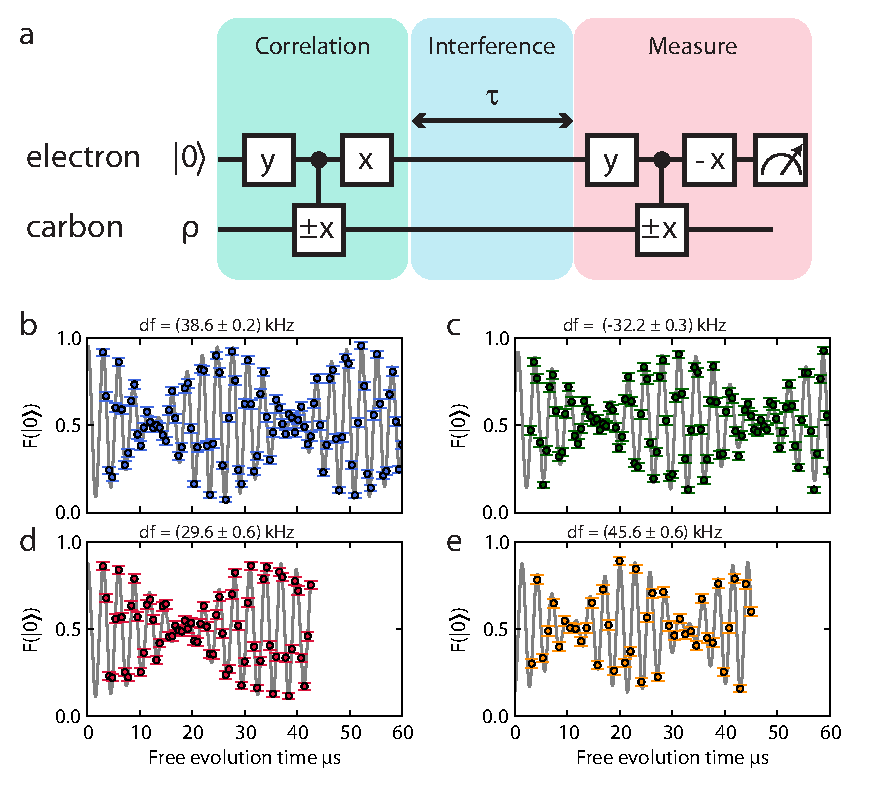
\includegraphics[width=130mm]{Fig2}
	\caption{\label{fig:cdl-fig2} \textbf{Characterization of single $^{13}C$ spins.} (a) Circuit diagram to determine $\omega_0$ and $\omega_1$ of individual $^{13}C$ spins via the electron spin. The conditional gates on the carbon spin are implemented using resonant dynamical decoupling techniques as explained in the main text. Because the evolution of the carbon spin is correlated with an eigenstate of the electron spin during the interference, a coherent signal can be observed even for $\tau \gg T^{*}_{2,electron}$ = (4.18 $\pm$ 0.01) $\mu$s (b)-(e) The resulting interference signal measured for four individual $^{13}C$ spins near a single NV-center. Grey lines are fits to the data with function $F = \frac{A}{2}\cos(\omega_0 \tau +\phi_0) + \frac{B}{2}\cos(\omega_1 \tau + \phi_1)$. We find $\omega_0$ /2$\pi$ = (326.0 $\pm$ 0.2), (325.9 $\pm$ 0.2), (325.1 $\pm$ 0.5), (325.9 $\pm$ 0.4) kHz (b-e), consistent with the gyromagnetic ratio of a $^{13}C$ spin in a field of (303 $\pm$ 1) G.  For the second frequency component we find $\omega_1$ /2$\pi$ = (364.6 $\pm$ 0.1), (293.7 $\pm$ 0.2), (354.7 $\pm$ 0.5), (371.5 $\pm$ 0.4) kHz. The data is taken with 500 repetitions per data point and the error bars correspond to one standard deviation.}
\end{figure*}

Because the hyperfine interaction is determined by the specific position of each nuclear spin relative to the NV center, the resonance condition for $\tau$ is different for each nuclear spin. We can thus characterize the nuclear spin environment\cite{Taminiau_Phys.Rev.Lett._2012} by preparing the electron in a superposition state and measuring the phase that is acquired when sweeping $\tau$. Here we select four individual $^{13}C$ spins to study in more detail, and design controlled gates following Taminiau et al.\cite{Taminiau_NatNano_2014}.

The nuclear spin dynamics are characterized by the nuclear spin precession frequencies $\omega_0$ and $\omega_1$  corresponding to the electron spin being in $m_s = 0$ and $m_s = 1$, respectively (see also Methods). To directly determine the frequencies $\omega_0$,  $\omega_1$ and $df = ( \omega_1 − \omega_0 )/2 \pi$  for each of the four nuclear spins we perform the experimental sequence\cite{Laraoui_NatCommun_2013} shown in Fig. \ref{fig:cdl-fig2}a. The electron is prepared in state $\rho_{0,e} = \ket{0}\bra{0}$, whereas the nuclear spin state is un-polarized (mixed state $\rho_{m.C} = (\ket{0}\bra{0} + \ket{1}\bra{1})/2$ ). The first set of gates correlates the electron state with the X-projection of the nuclear spin state, so that the state is $\rho_{0,e} \otimes \rho_{x,C} + \rho_{1,e} \otimes \rho_{-x,C}$ , with $\rho_{\pm X,C} = \ket{\pm X}\bra{\pm X}$ and  $\ket{\pm X} = (\ket{0}_C \pm \ket{1}_C)/\sqrt{2}$. The controlled nuclear spin rotations are realized by the pulse sequences described above, with $\tau$ resonant for that specific spin. Second, the nuclear spin evolves freely, either with $\omega_0$ or with $\omega_1$, depending on the electron state. Finally the phase accumulation of the nuclear spin is measured by correlating it to the electron spin before reading out the electron spin. 

The beating observed in the signal directly yields the frequency difference df and therefore the additional phase picked up due to the time the electron spent in $m_s = + 1$.   For the four spins we find $df = (29.6 \pm 0.6), (-32.2 \pm 0.3) (38.6 \pm 0.2)$ and $ (45.6 \pm 0.6) $  kHz respectively.  These values show that several nuclear spins with coupling strengths between approximately 20-50 kHz are readily available in diamond samples with a natural abundance of $^{13}C$.

\section{Modeling the dephasing of a carbon spin during entanglement generation}

We analyze the performance of $^{13}C$ spins as quantum memory in the context of  the  heralded entanglement protocol proposed by Barrett and Kok\cite{Barrett_Phys.Rev.A_2005}, which was implemented by Bernien et al.\cite{Bernien_Nature_2013}. The protocol is based on the creation of spin-photon entanglement at both nodes, followed by two-photon interference and measurement of these photons. The protocol is probabilistic since it is susceptible to photon loss. Importantly, successful generation of entanglement is heralded by the detection of the two photons and thus the sequence can be repeated until successful. 

Spin-photon entanglement is created using the following sequence (Fig. \ref{fig:cdl-fig3}a). The electron spin is prepared in state $\ket{0}_e$ by optical pumping (Fig. \ref{fig:cdl-fig1}d). Using microwaves the electron spin is then brought in a coherent superposition. Next, the NV center is optically excited with a short laser pulse that is only resonant if the spin is in state $\ket{0}_e$. Spontaneous emission generates a photon that is entangled with the state of the spin: $\ket{\Psi} = (\ket{0}_e \ket{1}_p +\ket{1}_e \ket{0}_p)/\sqrt{2}$  where $\ket{1}_p$ ($\ket{0}_p$)  denotes the presence (absence) of a photon. The goal is that the nuclear spin memory reliably stores quantum states during many repetitions of this sequence.

 \begin{figure*}
	\centering
	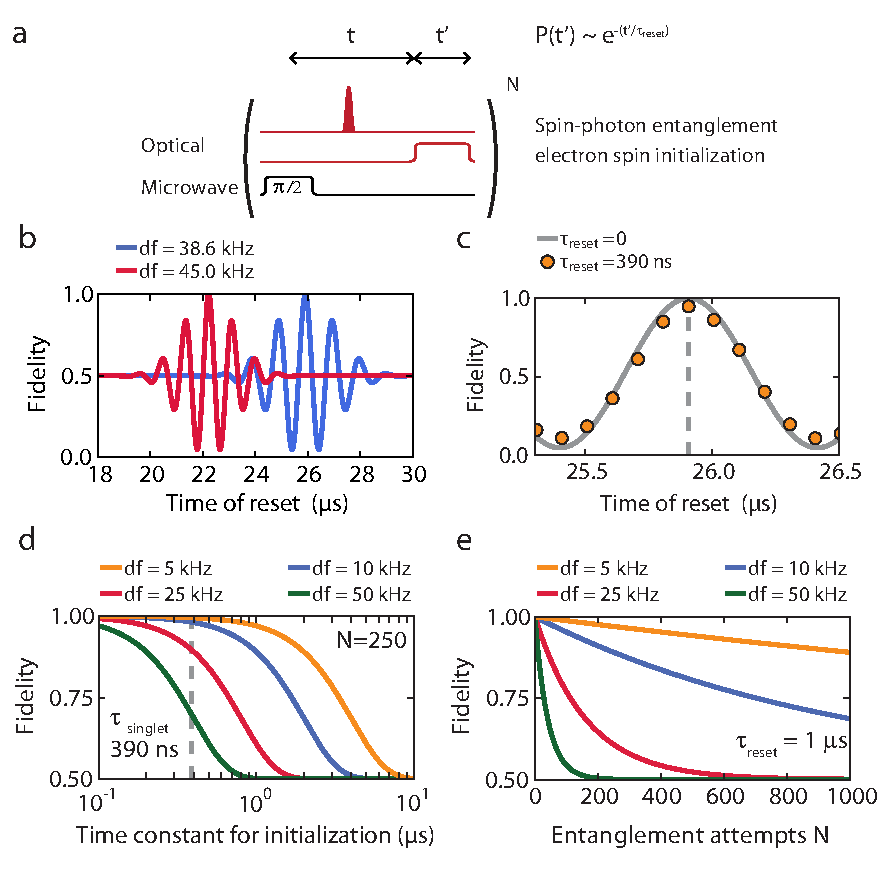
\includegraphics[width=130mm]{Fig3}
	\caption{\label{fig:cdl-fig3} \textbf{Simulations of the dephasing of a $^{13}C$ spin quantum memory while generating entanglement. } (a) Diagram for the protocol to create spin-photon entanglement. (b) Simulations of the fidelity for different $^{13}C$ spins after \textit{N} = 50 repetitions of the protocol, assuming that the reset is instantaneous ($t^{\prime}$ = 0, formula \ref{eq:CDL-deph} of main text). The initial state of a carbon spin can be perfectly preserved by choosing the time between the $\pi$/2-pulse and the reset to \textit{t} = 2$\pi$ /$d \omega$. (c) The effect of the spin pumping process on the fidelity of the memory after \textit{N} = 50 repetitions. Orange dots are a Monte-Carlo simulation where for every electron spin reset, a time $t^{\prime}$ is drawn from an exponential probability distribution with $\tau_{reset}$ = 390 ns. Grey line is a comparison with an ideal reset. $d \omega$ = (2$\pi$) 38.6 kHz. (d) Dependence of the memory fidelity on the characteristic reset time $\tau_{reset}$ using formula \ref{eq:CDL-deph_an}. (e) Dephasing of the memory as a function of entanglement attempts for different coupling strengths, fixing  $\tau_{reset}$ = 1 $\mu$s.}
\end{figure*}



The performance of a quantum memory can be characterized by its ability to store an unknown quantum state $\ket{\psi} = \alpha \ket{0}_C + \beta e^{i \phi}\ket{1}_C$. During the spin-photon entanglement sequences the phase $\phi$ of the nuclear spin state is affected in two ways. First, when the emitted photon is lost (heralding fails), the electron spin state is randomly projected into either $\ket{0}_e$ or $\ket{1}_e$ resulting in nuclear spin evolutions with $\omega_0$ or $\omega_1$, respectively. Second, before the next repetition, the electron spin is reset by optical pumping, a stochastic process that introduces a distribution of spin flip times. These two effects are now analyzed separately.

After a single round of optical excitation that generates spin-photon entanglement, the electron spin is projected into an unknown eigenstate if the photon is lost. The carbon spin acquires a phase $d \omega t$ if the electron is projected in $\ket{1}_e$, where $d \omega = 2 \pi df$ and \textit{t} the time at which the reset is applied. When this process is repeated \textit{N} times, the number of times \textit{k} that the electron is projected in $\ket{1}_e$ is given by a binomial distribution and the final state fidelity \textit{F} of the carbon spin state is given by:

\begin{equation}\label{eq:CDL-deph}
F = \frac{1}{2} + \frac{1}{2^{N+1}} \sum_{k=0}^{N} \binom{N}{k} \cos \lbrack k d \omega t \rbrack
\end{equation}

where the electron spin reset is taken to be instantaneous and we only consider the initial memory state is $\ket{\psi} = (\ket{0}_C + \ket{1}_C/\sqrt(2)$, which is most sensitive to dephasing. Fig. \ref{fig:cdl-fig3}b shows the calculated fidelity as a function of the time \textit{t}, for two carbon spins that were identified in Fig. \ref{fig:cdl-fig2}. For each carbon spin there is a unique condition at \textit{t} =2$\pi$ /$d \omega$, for which the phase is independent on the electron state resulting in \textit{F} = 1. Note that in the full entanglement protocol\cite{Bernien_Nature_2013,Barrett_Phys.Rev.A_2005} an electron $\pi$-pulse is applied between rounds of excitation, so that this phase difference can be cancelled for all \textit{t}. 


In reality the reset of the electron spin by spin pumping is a stochastic process involving multiple transitions to the optically excited state as well as mixing between multiple excited states. Here we model the dynamics of this process as an exponential distribution  $e^{- \frac{ t^{\prime} } {\tau_{reset} } }$  with a characteristic time $\tau_{reset}$.  In Fig. \ref{fig:cdl-fig3}c we compare the results of a monte-carlo simulation that includes the probabilistic reset time $t^{\prime}$ for $\tau_{reset}$ = 390 ns with the curve of equation \ref{eq:CDL-deph}. As expected the same behavior is observed, but the maximum fidelity is reduced since the stochastic reset leads to dephasing of the carbon spin. 

To analyze the effect of the electron spin reset on the nuclear spin in detail we now assume that  \textit{t} = 2$\pi$ $d\omega$ which allows us to derive an analytical expression for the fidelity of the carbon spin (see methods for the derivation of this result): 

\begin{equation}\label{eq:CDL-deph_an}
F = \frac{1}{2} + \frac{1}{2^{N+1}}\left(1 + e^{-\frac{1}{2}\tau_{reset} ^2 d\omega^2}\right)^N.
\end{equation}

In Fig. \ref{fig:cdl-fig3}d we plot the resulting memory fidelity after 250 entanglement repetitions versus the reset constant $\tau_{reset}$, for different values of \textit{df}. Although for an instantaneous reset ($\tau_{reset} \to 0$) the state can be perfectly preserved, a finite uncertainty in the reset time constant reduces the fidelity, with the effect being stronger for higher coupling strengths df. A natural lower limit to the reset time $\tau_{reset}$ is the slowest decay rate involved in the spin pumping process. For the NV center this is expected to be the singlet lifetime $\tau_{singlet} \approx$ 390 ns\cite{Doherty_PhysicsReports_2013}.  For this value, Fig. \ref{fig:cdl-fig3}d predicts that for coupling strengths of \textit{df} < 10 kHz the state can be preserved with a fidelity of > 98 \% even after 250 entanglement attempts. 

The reset constants currently reported in the literature are approximately 1 $\mu$s \cite{Bernien_Nature_2013}. In Fig. \ref{fig:cdl-fig3}e we plot the fidelity as a function of number of entanglement attempts for $\tau_{reset}$ = 1 $\mu$s. These calculations predict that 25 repetitions of the entanglement protocol will yield a fidelity of 90.3 \% for the lowest coupling strength found in Fig. \ref{fig:cdl-fig2}, which would already provide significant speed advantages in establishing entanglement links\cite{Campbell_Phys.Rev.Lett._2008}. For coupling strengths \textit{df} < 10 kHz, hundreds of repetitions become feasible. Such lower coupling strengths are available in isotopically purified diamonds\cite{Maurer_Science_2012}.

We emphasize that the model presented here does not include the detailed excited state dynamics of the spin pumping process. We expect that averaging over rapid spin flips and time spent in states with zero spin projection during these dynamics will further reduce actual dephasing. We therefore expect that our analysis sets a lower bound for the number of possible repetitions.

We have modelled the dephasing of nuclear spins quantum memories coupled to an NV electron spin that is repeatedly used to establish spin-photon entanglement. We find that nuclear spins with weak hyperfine couplings (20-50 kHz) are readily available in natural abundance diamonds. Our analysis shows that these spins can be used to store quantum states during 25 entanglement attempts with a fidelity of 90.3 \%, while nuclear spins in isotopically purified samples with coupling strengths below 10 kHz can even enable hundreds of repetitions. These results demonstrate that nuclear spins with weak hyperfine coupling strengths are promising quantum memories for quantum networks providing a route towards entanglement distillation and quantum repeaters.

\section{Methods}
We take the limit of $\gamma_C B \gg A_{\perp}$ (with $A_{\perp}$  the hyperfine component perpendicular to the static magnetic field) such that the eigenstates of the $^{13}$C-spin are independent of the electron and the only net effect of the electron-carbon coupling is that the carbon acquires a phase depending on the state of the electron. Choosing the rotating frame of the carbon resonant with the energy splitting for the electron in $\ket{0}_e$, the carbon state will acquire a phase $e^{id\omega t}$ for the electron in $\ket{1}_e$ (with $d \omega$ = 2$\pi$ \textit{df}) and does not evolve otherwise.

We derive an expression for the maximally achievable memory fidelity. The scheme of Fig 3a is repeated \textit{N} times. Phase errors occur if the electron spin has to be reinitialized by pumping it to another spin state. During every execution of the protocol, the electron spin is projected into $\ket{0}_e$ or $\ket{1}_e$ with equal probability. The probability for \textit{k} repumping events is then given by a binomial distribution

\begin{equation}
P_{ek} = \frac{1}{2^N}\binom{N}{k}
\end{equation}

Every time the electron is reset from $\ket{1}_e$ into $\ket{0}_e$ the memory spin will pick up a random phase $\delta \theta = d \omega (t^{\prime} - \tau_{reset})$ which is given by the difference between energy levels of the carbon spin conditional on the electron spin $d \omega$ and the deviation $(t^{\prime} - \tau_{reset})$ from the mean repumping time. The overall acquired phase for \textit{k}  repumping events is then the sum of the individual random phases. The fidelity with the initial memory state after \textit{N} repetitions is thus given by

\begin{equation}
F_k = \frac{1}{2}\left(1+\cos \left[\sum_{k=0}^N \delta \theta_k\right]\right)
\end{equation}

Under the assumption that the distributions for all repumping events are independent the problem can be seen as a random walk in accumulated repumping time. Each step of this random walk is then exponentially distributed around the mean repumping time $\tau_{reset}$. The probability distribution of the summed repumping time is given by\cite{Akkouchi_CCMS_2008}

\begin{equation}
P(t^{\prime}) = \frac{t'^{k-1}}{\tau_{reset}^k(k-1)! }e^{-t^{\prime}/\tau_{reset}} \approx \frac{1}{\sqrt{2\pi}\sigma}e^{-\frac{(t^{\prime}-\mu)^2}{2\sigma^2}}
\end{equation}


where we use the central limit theorem to approximate this distribution by a normal distribution with width $\sigma = \tau_{reset} \sqrt{k}$ and mean $\mu = \tau_{reset} k$ , as we are interested in solutions for a large number of repumping events. The expected fidelity after \textit{N} experimental runs is calculated by summing over the probability distributions for the electronic state and the corresponding accumulated repumping time

\begin{eqnarray}
F_N & = & \sum_{k=0}^N  P_{ek} \int F_k\, P(t^{\prime})\, dt^{\prime} \nonumber \\
& = & \frac{1}{2} + \frac{1}{2} \sum_{k=0}^N P_{ek} e^{-\frac{1}{2}k\tau_{reset}^2 d \omega^2} \nonumber \\
& = & \frac{1}{2} + \frac{1}{2^{N+1}}\left(1 + e^{-\frac{1}{2}\tau_{reset}^2 d \omega^2}\right)^N.
\end{eqnarray}

\newpage
\bibliographystyle{../thesis}
\bibliography{cdl}



\graphicspath{{./ch_carbon_dephasing_purified/figures/}}


\chapter{Storing a quantum state during optical excitation of a quantum network node}
\label{ch:CDP}

\begin{center} 
    \vspace{-1cm} {M.S.~Blok, K. ~van Bemmelen, N.~Kalb, A.~Reiserer, T.H.~Taminiau and R.~Hanson} 
\end{center}

\vspace{0.5cm} 

The ability to locally store a quantum state in a quantum network node while establishing entanglement with a distant node is a crucial prerequisite for implementing entanglement distillation, purification and quantum repeater protocols\cite{Bennett_Phys.Rev.Lett._1996,Campbell_Phys.Rev.Lett._2008,Briegel_Phys.Rev.Lett._1998,Childress_Phys.Rev.Lett._2006}. For quantum network nodes based on NV centers in diamond, nearby $^{13}$C-spins are a prime candidate for such a quantum memory. The challenge is that these nuclear spins have a constant coupling to the optically active electron spin, resulting in possible dephasing of the stored state when the electron is reset multiple times as required for generating remote entanglement. In chapter \ref{ch:CDL} we discussed an analytical model to describe this process and found that nodes with low electron-nuclear coupling strength and fast electron reset are expected to provide the best performance. Here we present preliminary experimental results to test our model in an isotopically purified sample where $^{13}$C-spins with coupling strengths of < 1 kHz can be located and controlled. We find that multiple resets of the electron spin indeed induce dephasing of the nuclear-spin quantum memory and that this process can be suppressed by reducing the electron reset time. While the data qualitatively agrees with our model, the observed dephasing rate is faster than predicted indicating that we are limited by an additional decoherence process. Nonetheless our results show that a $^{13}$C-spin allows for the storage of a quantum state during 200 repetitions with very little loss of fidelity ($99 \%$ fidelity with initial state).
\clearpage

Here we investigate the ability of a weakly coupled $^{13}$C-spin to store a quantum state while optically addressing the electron spin to generate remote entanglement (as presented in chapter \ref{ch:LDE}). Since this protocol \cite{Barrett_Phys.Rev.A_2005,Bernien_Nature_2013} is inherently probabilistic it must be repeated many times until success, requiring the electron spin to be reset before each repetition. Because the exact time of our reset method is uncertain (the optical pumping is a stochastic process) and electron-nuclear interaction is constant, this can induce dephasing of the nuclear spin memory. From the simulations presented in chapter \ref{ch:CDL} we conclude that this dephasing process can be suppressed by using relatively distant $^{13}$C-spins with low hyperfine coupling and implementing a fast reset that minimizes the time-uncertainty. To locate distant $^{13}$C-spins we use an isotopically purified diamond (0.01 $\%$ $^{13}$C) and show that we can control nuclear spins with a hyperfine coupling constant in the order of $\sim$ 200 Hz. We characterize the reset timescale by varying the time and the power of the repumping laser pulse. Finally we measure the dephasing of the nuclear spin as a function of number of times that the electron spin is reinitialized.

\section{Controlling a weakly coupled $^{13}$C-spin in isotopically purified diamond.}

We detect weakly coupled $^{13}$C-spins in the vicinity of an NV center via the electron spin using dynamical decoupling spectroscopy\cite{Taminiau_Phys.Rev.Lett._2012,Zhao_NatNano_2012,Kolkowitz_Phys.Rev.Lett._2012}. In Fig. \ref{fig:cdp-fig1}a we vary the time between $N = 128$ equally spaced $\pi$-pulses on the electron initially prepared in an equal superposition and plot the probability of recovering $m_s = 0$ after a final $\pi$/2-pulse. The observed periodical collapses\cite{Childress_Science_2006} are well explained by the interaction of the electron spin with a $^{13}$C-spin bath in a magnetic field of 22.7 $G$. We align the magnetic field along the quantization axis of the NV-center by minimizing the average of the $m_s = 0 \rightarrow -1$ and $m_s = 0 \rightarrow +1$ transitions. From these measurements we find a magnetic field $B_z = (22.5 \pm 0.1) $ G and $B_x = (2.4 \pm 2) $ G.

In a higher resolution measurement around the second collapse (Fig. \ref{fig:cdp-fig1}b) we observe two additional resonances associated with single $^{13}$C-spins. The location and shape of these resonances are determined by the hyperfine parameters of the carbon spin\cite{Taminiau_Phys.Rev.Lett._2012}. By comparing the data with simulations of the electron-nuclear interaction we estimate hyperfine constants of $A_{\parallel,C} = 220$ Hz and $A_{\perp,C} = 200$ Hz ($A_{\parallel,C} = -1.02$ kHz and $A_{\perp,C} = 190$ Hz) as plotted in red (green). In comparison, previous experiments have demonstrated control of strongly coupled $^{13}$C-spins with interaction strengths between $\sim$ 100 - 1 MHz \cite{Jelezko_Phys.Rev.Lett._2004,Dutt_Science_2007,Pfaff_NatPhys_2013,Neumann_Science_2008} and weakly coupled nuclear spins in the order of 50-30 kHz \cite{Taminiau_NatNano_2014} in natural abundance samples. In isotopically purified samples, manipulation of a strongly coupled 2.6 kHz $^{13}$C-spin was demonstrated\cite{Maurer_Science_2012}.

 \begin{figure*}
	\centering
	\includegraphics[width=130mm]{Fig1}
	\caption{\label{fig:cdp-fig1} \textbf{} (a) Dynamical Decoupling spectroscopy of the $^{13}$C-spin bath. Grey lines are the expected collapses of the signal due to interaction with the $^{13}$C-spin bath. They occur at $\tau_k = \frac{\pi(2k-1)}{2\omega_L}$, with $k = 1,2,3...$ the order of the resonance and $\omega_L$ the larmor frequency of the $^{13}$C spins.(b) Two $^{13}$C-spins can be identified, red (green) line is a simulation of the resulting signal for the interaction with a single spin with hyperfine constants of $A_{\parallel,C} = 220$ Hz and $A_{\perp,C} = 200$ Hz ($A_{\parallel,C} = -1.02$ kHz and $A_{\perp,C} = 190$ Hz), plotted in red: carbon 1 (green: carbon 2). (c) Free induction decay of carbon 1 with and without repetitive reset }
\end{figure*}

We control an individual $^{13}$C-spin by applying $\pi$-pulses to the electron spin and by choosing the time between the pulses on resonance with the electron-nuclear coupling \cite{Taminiau_Phys.Rev.Lett._2012,Taminiau_NatNano_2014}. This results in a rotation of the nuclear spin conditional on the initial electron spin state, hence by choosing the initial state of the electron we can construct one-, and two-qubit gates. The $^{13}$C spin is initialized and measured by entangling the electron and nuclear spin and subsequent readout of the electron spin. In Fig. \ref{fig:cdp-fig1}c we show a Ramsey measurement of carbon 1. By measuring the precession frequency of the carbon spin depending of the electron spin state we find the frequency difference $df = (227 \pm 6)$Hz. This parameter is expected to be relevant for the nuclear spin dephasing rate upon repetitive reset of the electron spin as discussed in chapter \ref{ch:CDL}. The free induction decay of the nuclear spin is measured for the electron spin in an eigenstate (Fig. \ref{fig:cdp-fig1}c right panel) and when the electron spin is reset every $\sim$ 12 $\mu$s (Fig. \ref{fig:cdp-fig1}c left panel). By comparing the resulting decoherence times $T_{decay}$, we find that repetitive reset of the electron spin reduces the coherence time roughly with a factor of 50. From equation \ref{eq:CDL-deph_an} we find the product of the frequency difference $df$ and the reset time $\tau_{reset}$ to set the timescale of dephasing. We therefore now characterize the optical spin-pumping process of the electron.



\section{Fast optical reset of the electron spin.}

To measure the time required to reset the electron spin we prepare $m_s= -1$ and plot the probability to prepare $m_s = 0$ after applying an optical pulse on the $E^{\prime}$ transition for a variable time (Fig. \ref{fig:cdp-fig2}a). We find that the data can be fitted to a double exponential function, consistent with previous measurements of the fluorescence during optical repumping on $E_y$ and $A_1$\cite{Bernien_Nature_2013}. This indicates that the spin pumping process involves transitions to multiple levels in the excited state, such as the meta-stable singlet state. In Fig. \ref{fig:cdp-fig2}b we plot the largest of the two time constants obtained from the fits in Fig. \ref{fig:cdp-fig2}a as a function of laser power. For low laser power the reset time is likely to be limited by the excitation rate to the excited state. Increasing the laser power significantly reduces the reset time until it saturates around 200 ns, which could indicate that here the spin pumping is limited by the lifetime of the meta-stable singlet state \cite{Doherty_PhysicsReports_2013}.

For a 500 nW repump pulse we find that the electron spin can be reset within a microsecond, with a characteristic time constant $\tau_{reset} = (220 \pm 27) $ ns. Apart from reducing dephasing of the nuclear spin due to electron spin flips, this also allows for an increased entanglement generation rate since the repetition rate of the experiments presented in chapter \ref{ch:LDE} was limited by the 5 $\mu$s repump pulse. However in figure $\ref{fig:cdp-fig2}$ the electron spin is reset once, while the heralded entanglement protocol requires repetitive initialization steps. We find that for repetitive electron initialization with a 500 nW pulse there is a significant probability to ionize the NV center after several hundreds of repetitions. We therefore now analyze the carbon dephasing for a maximum laser power of 100 nW where no significant ionization is observed.

 \begin{figure*}
	\centering
	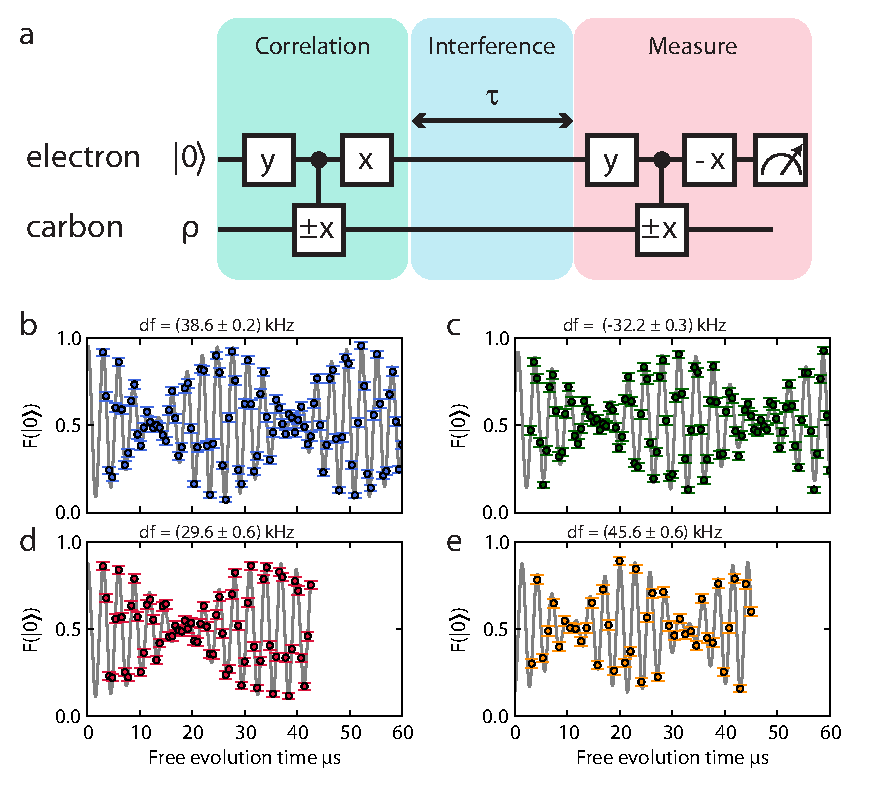
\includegraphics[width=130mm]{Fig2}
	\caption{\label{fig:cdp-fig2} \textbf{Reset of the electron spin} (a) Measurement of the timescale of the reset process. Plotted is the probability of preparing $m_s = 0$ after preparing $m_s = -1$ as a function of repump time and power. Solid lines are fits to the function $S = o - A e^{-\frac{x-x_o}{\tau_{reset}}}-(1-A) e^{-\frac{x-x_o}{\tau_{reset,2}}}$ (b) Largest of the two fitted time constant of the reset process as a function of reset power.}
\end{figure*}

\section{Dephasing of a carbon spin upon optical excitation of the electron spin.}

 We demonstrate the robustness of the carbon spin quantum memory by measuring its ability to store a coherent quantum state while performing the local operations for generating heralded entanglement on the electron spin (Fig. \ref{fig:cdp-fig3}). We prepare carbon spin 1 in a maximum superposition $\ket{\psi}=(\ket{0}_C + \ket{1}_C)/\sqrt{2}$ and perform state tomography after a variable number of protocol repetitions (sequence on electron spin is ($\pi/2 - \pi -$ reset)$^N$, see Fig. \ref{fig:LDE-fig1-protocol}). We omit the two optical $\pi$-pulses to generate spin-photon entanglement. We expect their influence on the carbon spin to be negligible since they effectively perform a measurement of the electron spin which in this case can be incorporated into the reset.
 \begin{figure*}
	\centering
	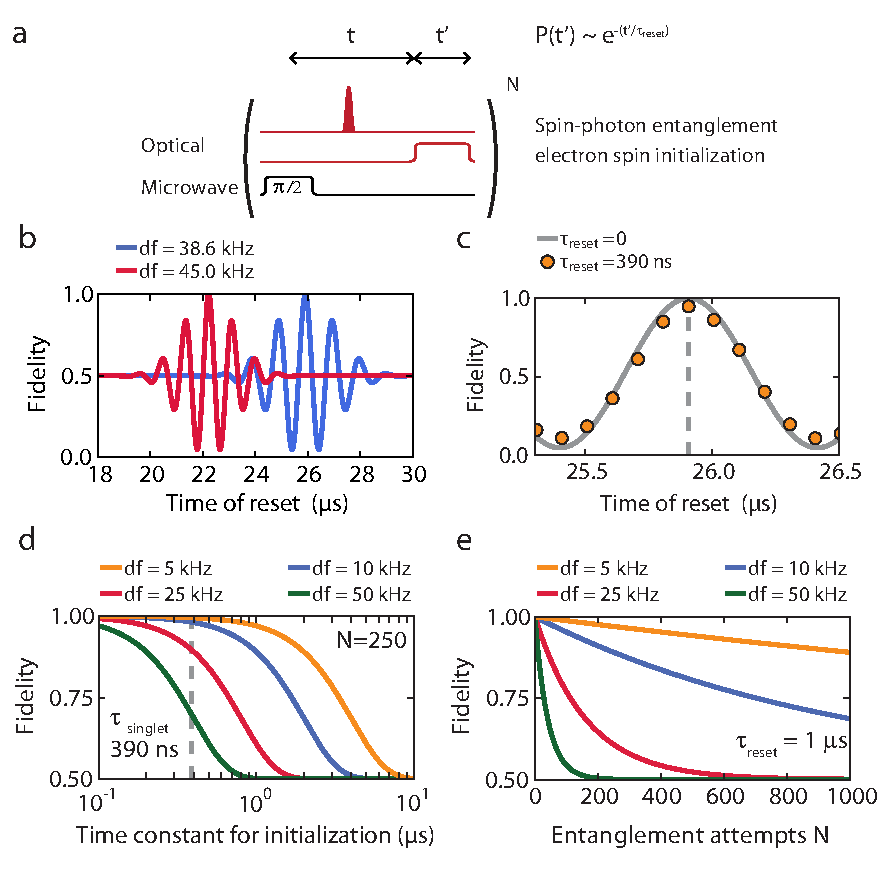
\includegraphics[width=130mm]{Fig3}
	\caption{\label{fig:cdp-fig3} \textbf{} (a) Tomography of carbon spin 1 initially prepared in a superposition as a function of number of repetitions of the heralded entanglement protocol. The repumping pulse is applied for 20 $\mu$s with a power of 100 nW, the time before and after the microwave $pi$-pulse is 200 ns. (b) Dephasing of the carbon spin for different repumping powers, with the same repump time and interpulse delay as in (a). Inset: the decay constants obtained from a fit to the data in (b) as a function of $\tau_{reset}$ for that laser power. }
\end{figure*}

In Fig. \ref{fig:cdp-fig3}a we show that after 200 repetitions the initial state is almost perfectly recovered for 100 nW repump power ($\tau_{reset} = (870 \pm 100)$ ns). The oscillation in the XY-plane of the Bloch sphere is due to the larmor precession of the carbon spin. In a realistic protocol where the number of required repetitions is probabilistic, this oscillation can be correct with real-time feedback. We therefore take the quadratic sum of the expectation values $<X>_C$ and $<Y>_C$ as a figure of merit and find that this quantity is preserved with a fidelity of $(99 \pm 1) \%$ after 200 repetitions.

Strikingly when we plot the full decay curve (Fig. \ref{fig:cdp-fig3}b) we find that the signal is best fitted with a Gaussian as opposed to an exponential function as expected from equation \ref{eq:CDL-deph_an}. Furthermore, while the measured decay constants for variable reset duration (inset of \ref{fig:cdp-fig3}b) can be fitted to the model, they are two orders of magnitude smaller than expected from the independently measured reset time and coupling constant. Since the decoherence rate is also faster than the intrinsic $T_2^{*}$ of the carbon spin, we conclude that the electron reset induces an additional decoherence process that is not included in our model. One hypothesis is that the perpendicular component of the hyperfine interaction ($A_{perp}$, neglected in chapter \ref{ch:CDL}) induces dynamics that lead to a $T_1$-type of decay. This can be verified by measuring the decay of an eigenstate of the carbon spin upon repumping the electron spin. Secondly the model simplifies the spin pumping process which in reality involves multiple transitions in the excited state. 

These experiments establish weakly coupled carbon spins as promising candidates for a memory in a quantum network node based on NV centers. Although further measurements are required to understand the limiting decoherence mechanism, the ability to store a quantum state for hundreds of repetitions can significantly improve the rate at which remote entanglement is established. These results show that in an isotopically purified diamond it is possible to preserve the coherence of a carbon spin during 200 repetitive resets of the electron spin. This is the maximum number of consecutive attempts to generate remote entanglement in previous experiments with NV centers\cite{Bernien_Nature_2013,Pfaff_Science_2014}. However, in protocols that aim to improve the entangling rate by using a quantum memory, the overhead associated with gates on the memory needs to be taken into account. Finding an optimal carbon spin for a quantum memory therefore poses a trade-off between its robustness against optical excitation of the electron spin and the gate-time, since the minimum time required to perform a gate between the nuclear spin and the electron spin is inversely proportional to the coupling strength. Furthermore, all errors in preparing and storing a state in the carbon spin will propagate to the resulting remote entanglement fidelity and therefore the carbon manipulation needs to be improved. In future work the incorporation of a quantum memory in a local node could be combined with the experiments presented in chapter \ref{ch:LDE} to demonstrate entanglement purification\cite{Campbell_Phys.Rev.Lett._2008} and eventually quantum repeaters \cite{Briegel_Phys.Rev.Lett._1998}.

\clearpage
\bibliographystyle{../thesis}
\bibliography{cdp}




\graphicspath{{./ch_conclusion_and_outlook/figures/}}

\chapter{Conclusions and outlook}
\label{ch:conclusion}

\begin{center} 
    \vspace{-1cm} {M.S. ~Blok} 
\end{center}

Future quantum technologies have the potential to have great impact on the fields of computation, communication and metrology. The work presented in this thesis capitalizes recently developed low temperature control techniques of the NV center in diamond to study quantum measurements and implement real-time feedback protocols. This transition from open-loop control to feedback control experiments will aid the development of diamond-based quantum technologies. In this chapter we give an overview of the main results and conclusions and provide an outlook for future research directions.
\clearpage

\section{Summary}
The results of this thesis can be summarized as follows.
\begin{itemize}

  \item A variable-strength measurement of the nitrogen spin of an NV center can be implemented via the electron spin. The backaction of sequential variable-strength measurements can be used to manipulate the nitrogen spin when digital feedback is incorporated.

  \item The advantage of adaptive frequency estimation protocols using the electron spin of a NV center is that fewer measurements are required to reach the same sensitivity compared to the best non-adaptive protocols. When overhead is included in the analysis this results a more accurate estimation at any fixed measurement time.

  \item Two electron spins in spatially separated diamonds can be entangled by performing a joint measurement of photons originating from the two NV centers. 

  \item Remote entanglement between two NV centers established via an heralded protocol can be used to unconditionally teleport the state of a nuclear spin to a distant electron spin.

  \item Weakly-coupled carbon spins in an isotopically purified diamond can maintain their coherence even after 200 repetitive resets of the electron spin.
  
\end{itemize}

This thesis reports the first experiments with spins in diamond where measurement outcomes are used as input for subsequent control operations thereby closing the loop between measurement and control. Furthermore they establish NV centers as a leading platform for building quantum networks.  Other systems are of course being developed in parallel and like spins in diamond each has their advantages and disadvantages. Recent advances include generation of remote entanglement between trapped ions \cite{Moehring_Nature_2007} and atoms\cite{Hofmann_Science_2012,Ritter_Nature_2012} and atomic ensembles\cite{Chou_Nature_2005} and the implementation of real-time feedback protocols using superconducting circuits\cite{Vijay_Nature_2012,Riste_Nature_2013} and photons \cite{Gillett_Phys.Rev.Lett._2010,Sayrin_Nature_2011}. The following sections will provide an outlook for future research directions with NV centers in diamond.

\section{Quantum Information Processing with NV centers in diamond}
A scalable solution for implementing quantum information technology with NV centers remains a long-term goal and making predictions of how this technology can be developed unavoidably contains some speculation. However it is possible to identify short-term challenges and provide possible solutions to overcome them. The demands on the system will depend on the application. A quantum computer will probably require a vast amount of physical qubits, while a big challenge for a quantum internet lies in entangling nodes with a relatively small amount of qubits over large distances. I will first discuss the challenge of locally scaling up the number of qubits and then proceed to connecting remote quantum nodes.

One challenge that can be overcome using real-time feedback is to protect quantum states against errors. A promising way to deal with noisy operations is to redundantly encode a logical qubit in multiple physical qubits and detect errors by measuring joint properties of the physical qubits without destroying the logical state. When an error is detected it can be corrected with real-time feedback based on the outcome of the multi-qubit measurements. This measurement based quantum error correction has recently been implemented using three weakly coupled $^{13}$C-spins and the quantum non-demolition measurement of the electron spin presented in chapter \ref{ch:AMC} to correct for one type of error\cite{Cramer_arXiv_2015}. The next step is to increase the number of encoding qubits to protect against arbitrary errors and to improve the gate fidelities to reach the scalability threshold. Higher gate fidelity could be achieved using asymmetrical dynamical decoupling sequences\cite{Casanova_arXiv_2015} or via numerical optimization \cite{Liu_NatCommun_2013,Dolde_NatCommun_2014}. Using dynamical decoupling spectroscopy techniques it has been demonstrated that six individual carbons can be identified\cite{Taminiau_Phys.Rev.Lett._2012}. It is still an open question how many carbon spins can be controlled with the electron spin. However it seems impractical to control a large amount of carbon spins via a single electron spin because all operations need to be applied sequentially and optimizing gates will become increasingly difficult for larger systems.

A promising way to engineer a scalable system is to adopt a modular approach where individual nodes consisting of one electron spin and a few nuclear spins are entangled using the optical interface. A recent proposal to implement the surface code using this quantum network architecture showed that the error thresholds of the entanglement generation can be reasonably high (10\%) if the local error rates for initialization, control and measurement are in the order of a percent\cite{Nickerson_NatCommun_2013}. For this approach the heralded entanglement protocol as presented in chapter \ref{ch:LDE} would have to be improved, given the current entanglement rate of 1/250 s$^{-1}$. To this end the NV center can be placed in a fiber-based micro cavity to enhance the photon collection efficiency and the emission in the zero phonon line via the Purcell effect\cite{Kaupp_Phys.Rev.A_2013,Albrecht_Phys.Rev.Lett._2013,Janitz_arXiv_2015}. When a highly connected quantum network is realized it would also lend itself for performing measurement-based quantum computing\cite{Raussendorf_Phys.Rev.Lett._2001,Benjamin_Laser&Photon.Rev._2009} where highly entangled graph states are first created and then the computation is performed by adaptive measurements.

To increase the separation between nodes in a quantum network for quantum communication one needs to overcome the optical losses. For photons emitted in the zero phonon line (wavelength 637 nm) the attenuation in an optical fiber is in the order of 12 dB/km. In a recent result entanglement over a distance of 1.3 km between two NV centers has been demonstrated\cite{Hensen_arXiv_2015}. In this experiment the entanglement rate was severely reduced by losses in the fiber. One way to overcome this is to downconvert the photons to telecom wavelength as was recently demonstrated with quantum dot emission\cite{DeGreve_Nature_2012,Zaske_Phys.Rev.Lett._2012}. Furthermore by employing weakly coupled nuclear spins as memories, entanglement purification\cite{Campbell_Phys.Rev.Lett._2008} and quantum repeater protocols\cite{Briegel_Phys.Rev.Lett._1998} can improve the efficiency of probabilistic entanglement generation.

\section{Single spin sensors}
Employing NV centers in diamond as quantum sensors \cite{Taylor_NatPhys_2008,Schirhagl__2014} has gained a lot of interest since the electron spin is sensitive to many physical quantities like as temperature\cite{Acosta_Phys.Rev.Lett._2010,Toyli_PNAS_2013}, strain\cite{Ovartchaiyapong_NatCommun_2014} and electric and magnetic fields\cite{Taylor_NatPhys_2008,Dolde_NatPhys_2011} with very high spatial resolution. There are several methods to bring the NV center close to the sample. The use of shallow NV centers in bulk diamond has enabled the detection of Johnson noise\cite{Kolkowitz_Science_2015} and spin waves\cite{vanderSar_NatCommun_2015} as well as the magnetic field of biological samples\cite{LeSage_Nature_2013}. Alternatively an NV center can be embedded at the end of a sharp tip that is scanned across the sample\cite{Balasubramanian_Nature_2008,Maletinsky_NatNano_2012,Rondin__2012,Pelliccione_Phys.Rev.Applied_2014,Haberle_NatNano_2015}. Finally NV centers in 
 nanocrystals with a size of a few nanometer can be used and it has been shown that they can be inserted into living cells\cite{Kucsko_Nature_2013}. A severe limitation of shallow NV centers is that surface effects can significantly deteriorate the stability of NV centers since nearby charge can lead to a conversion to NV$^-$ and magnetic noise reduces the coherence times of the spins. It was recently shown that a combination of surface treatment and annealing can improve the optical stability of shallow NV centers in bulk diamond\cite{Chu_NanoLett._2014}.

\section{Fundamentals of quantum mechanics}

Bell \cite{Hensen_arXiv_2015}
reality of wavefunction \cite{Pusey_NatPhys_2012}
weak measurements \cite{Aharonov_Phys.Rev.Lett._1988} toin coss \cite{Ferrie_Phys.Rev.Lett._2014} contextuality \cite{Pusey_Phys.Rev.Lett._2014}
gravitational collapse (\cite{Diosi_PhysicsLettersA_1987}, \cite{Penrose_Phil.Trans.R.Soc.Lond.A_1998}) exp with NV (\cite{Wezel_Proc.R.Soc.A_2012})

\bibliographystyle{../thesis}
\bibliography{conclusions}


\backmatter
%\chapter{Summary}

Gaining precise control over quantum systems is crucial for applications in quantum information processing and quantum sensing and to perform experimental tests of quantum mechanics. The experiments presented in this thesis implement quantum measurements and real-time feedback protocols that can help to achieve these goals using single electron and nuclear spins in diamond. Spins associated with the Nitrogen Vacancy (NV) center in diamond recently emerged as an excellent testbed to demonstrate quantum effects and are a promising building block for future quantum technology.\\

The NV center is an atomic defect in the diamond lattice consisting of a substitutional nitrogen atom next to an empty lattice site. With its effective electron spin and nearby nuclear spins it forms a natural multi-qubit register with long-lived spin states that can be manipulated with magnetic resonance techniques. At temperatures below 10 K it displays spin-selective optical transitions that can be individually addressed and thereby provide an optical interface enabling high-fidelity single-shot readout and the generation of spin-photon entanglement.\\

In chapter 3 the fundamental trade-off between information gain and state disturbance associated with a quantum measurement is investigated. A variable strength measurement of the nuclear spin associated with the host nitrogen atom is implemented via an indirect measurement using the electron spin. The measurement strength can be tuned by varying the amount of entanglement between the two spins. To avoid dephasing of the nuclear spin, due to spin-flips of the electron spin during its readout, a dynamical-stop readout is used to perform a QND measurement of the electron spin. This enables sequential partial measurements that can manipulate the nuclear spin using only the backaction of quantum measurements combined with real-time feedback. \\

The electron spin can be used to sense static magnetic fields by performing repetitive Ramsey sequences. The experiments presented in chapter 4 address the open question whether adaptive measurements can out-perform non-adaptive protocols for sensing applications. An adaptive strategy is implemented where the readout basis is optimized in real-time using a Bayesian estimation based on previous measurement outcomes. The experiment shows that this adaptive protocol outperforms the best known non-adaptive protocol when overhead is taken into account.\\

The results in chapter 5 demonstrate the generation of measurement-based entanglement between two electron spins separated by 3 meters. By locally entangling each electron spin with a photon and performing a subsequent joint measurement of the photons, entanglement between the electron spins is heralded. The generated Bell-pair shared between remote locations is then used to unconditionally teleport the state of a nuclear spin in one diamond to the electron spin in the other diamond. To this end the nuclear spin is prepared in the state that is to be teleported followed by a local measurement of the electron and nuclear spin in the Bell-basis. This measurement projects the electron spin in the other diamond to the initial state of the nuclear spin up to a unitary operation that depends on the outcome of the Bell-state measurement. The original state is then recovered via a feed-forward operation. The fact that the protocol to prepare the remote Bell-pair is heralded and that the local Bell-state measurement can distinguish all four Bell-states, allows for unconditional teleportation. \\

The final two chapters of this thesis discuss the use of weakly coupled $^{13}$C spins as a quantum memory that is robust against optical excitation of the electron spin. The ability to store a quantum state in a quantum register while remotely connecting it to other registers enables the implementation of entanglement purification and quantum repeater protocols. A theoretical model is introduced to analyze the dephasing of a carbon spin during repetitive resets of the electron spin (which is required in the presented heralded entanglement protocol). This model is then tested experimentally in an isotopically purified diamond with a carbon spin that is relatively insensitive to perturbations induced by electron spin-flips owing to its low coupling strength (200 Hz). Although the observed dephasing is stronger than predicted by the model the results indicate that it is possible to store a quantum state in the $^{13}$C spin while optically exciting the electron spin.

\chapter{Samenvatting}

Het nauwkeurig controleren van quantum systemen is essentieel zowel voor toepassingen in quantum informatica en quantum sensoren als voor experimentele tests van de quantum mechanica. De experimenten die in dit proefschrift worden beschreven, introduceren quantum metingen en terugkoppeling protocollen met enkele spins in diamant om deze doelen te bereiken. Spins nabij het stikstof-holte (nitrogen-vacancy, NV) centrum in diamant zijn uiterst geschikt om quantum effecten te demonstreren en zijn een veelbelovende bouwsteen voor toekomstige quantum technologie. \\

Het NV centrum is een atomisch defect in het diamant rooster bestaande uit een stikstofatoom in plaats van een koolstofatoom en een ontbrekend koolstofatoom op een naburige roosterplek. Met zijn elektron spin en nabijgelegen kernspins vormt het NV centrum een quantum register bestaande uit spins met lange coherentietijden die gemanipuleerd kunnen worden met magnetische resonantie technieken. Bij temperaturen beneden de 10 K vertoont het NV centrum spin-selectieve optische transities die individueel aangeslagen kunnen worden. Op deze manier kan de electron spin zeer betrouwbaar worden geinitialiseerd, gemeten en verstrengeld met een foton. \\

In hoofdstuk 3 wordt de fundamentele balans tussen het verkrijgen van informatie en het verstoren van een quantum toestand die hoort bij een quantum meting onderzocht. Door de kernspin te meten via de elektron spin kan de sterkte van de meting gevarieerd worden. Hierbij bepaalt de mate van verstrengeling tussen de twee spins de meetsterkte. Een nieuw ontwikkelde QND meting van de elektron spin kan decoherentie van de kernspin tijdens de uitlezing van de elektron spin verminderen. Dankzij deze QND meting kunnen opeenvolgende gedeeltelijke metingen op de kernspin worden gedaan. Tot slot laten we zien dat de terugslag van opeenvolgende gedeeltelijke metingen gebruikt kan worden om de toestand van de kernspin te manipuleren door gebruik te maken van tergkoppeling.\\

De elektron spin kan worden gebruikt om statische magnetische velden te meten door opeenvolgende Ramsey sequenties uit te voeren. De experimenten die besproken worden in hoofdstuk 4 richten zich de open vraag of het gebruik van terugkoppeling kan helpen om een quantum sensor te verbeteren. In het gedemonstreerde protocol met terugkoppeling wordt de meetbasis van de elektron spin geoptimaliseerd door een Bayesiaanse schatting te maken van het magneetveld gebaseerd op de voorgaande meetuitkomsten. De experimenten tonen aan dat het gebruik van terugkoppeling voordelig is wanneer men de \textit{overhead} meerekent.\\

De resultaten in hoofdstuk 5 demonstreren dat twee elektronen spins in diamanten op een afstand van 3 meter met elkaar verstrengeld kunnen worden door middel van metingen. Door de individuele elektronen spins lokaal te verstrengelen met een foton en vervolgens de fotonen gezamenlijk te meten, worden de elektronen spins in een verstrengelde toestand geprojecteerd. Het resulterende Bell-paar dat gedeeld wordt tussen de twee locaties wordt gebruikt om de toestand van een kernspin in de ene diamant te teleporteren naar een elektron spin in de andere diamant. Hiertoe wordt de kernspin in de te verzenden toestand gebracht waarna de kernspin en de elektron spin lokaal gemeten worden in de Bell-basis. Door het resultaat van deze meting via een klassiek kanaal te communiceren naar de ontvangst locatie kunnen we met terugkoppeling de elektron spin in de andere diamant in de gewenste toestand brengen. \\

In de laatste twee hoofdstukken van dit proefschrift wordt de mogelijkheid onderzocht om zwak gekoppelde $^{13}$C spins te gebruiken als een quantum geheugen dat robuust is tegen verstoringen die kunnen optreden wanneer de elektron spin optisch aangeslagen wordt. Het vermogen om een quantum toestand op te slaan in een quantum register terwijl het tegelijkertijd verstrengeld wordt met een ander register maakt het mogelijk om \textit{entanglement purification} en \textit{quantum repeater} protocollen te implementeren. In een theoretisch model wordt de decoherentie van de koolstof spin beschreven wanneer de elektron spin herhaaldelijk geinitialiseerd wordt (net zoals in het hierboven genoemde protocol om elektronen over afstand te verstrengelen). Dit model wordt getest in een diamant met relatief weinig $^{13}$C isotopen waarin de koolstof spins dankzij hun lage koppelingssterkte (200 Hz) minder gevoelig zijn voor verstoringen door de elektron spin. Hoewel de waargenomen decoherentie sterker is dan het model voorspelt, laten de resultaten zien dat het mogelijk is om een quantum toestand op te slaan in een $^{13}$C spin terwijl het elektron optisch aangeslagen wordt.



%\chapter{Acknowledgements}


%\chapter{List of Publications}
\interfootnotelinepenalty=10000

\begin{enumerate} % [leftmargin=0pt,labelsep=.6in]
\nohyphens{


\item {\em Repeated quantum error correction on a continuously encoded qubit by real-time feedback.} \\
J.~Cramer, N~Kalb, M.A.~Rol, B.~Hensen, M.S.~Blok, M.~Markham, D.J.~Twitchen, R.~Hanson and T.H.~Taminiau. \\
\textit{In preparation}.

\item {\em Optimized quantum sensing with a single electron spin using real-time adaptive measurements.} \\
C. Bonato$^*$, M.S. Blok$^*$, H.T. Dinani, D. Berry, M.~Markham, D.J.~Twitchen, R. Hanson. \\
Nature Nanotechnology \textit{In press}, doi:10.1038/nnano.2015.261 (2015).
{\renewcommand{\thefootnote}{}\footnote{$^*$Equally contributing authors}}

\item {\em Loophole-free Bell inequality violation using electron spins separated by 1.3 kilometres.}
B.~Hensen, H.~Bernien, A.E.~Dréau, A.~Reiserer, N.~Kalb, M.S.~Blok, J.~Ruitenberg, R.F.L.~Vermeulen, R.N.~Schouten, C.~Abellán, W.~Amaya, V.~Pruneri, M.W.~Mitchell, M.~Markham, D.J.~Twitchen, D.~Elkouss, S.~Wehner, T.H.~Taminiau and R.~Hanson. \\ 
Nature \textit{In press}, doi:10.1038/nature15759 (2015).

\item {\em Towards quantum networks of single spins: analysis of a quantum memory with optical interface in diamond.}\\
M.S.~Blok$^*$,N.~Kalb$^*$, A.~Reiserer, T.H.~Taminiau and R.~Hanson.  \\
Faraday Discussions \textit{Advanced online publication}, doi:10.1039/c5fd00113g (2015).

\item  {\em Unconditional quantum teleportation between distant solid-state qubits.} \\
W.~Pfaff, B.~Hensen, H.~Bernien, S.~van Dam, M.S.~Blok, T.H.~Taminiau, M.J.~Tiggelman, R.S.~Schouten, M.~Markham, D.J.~Twitchen, and R.~Hanson.\\
Science \textbf{345}, 532-535 (2014).

\item {\em Manipulating a qubit through the backaction of sequential partial measurements and real-time feedback.} \\
 M.S.~Blok$^*$, C.~Bonato$^*$, M.L.~Markham, D.J.~Twitchen, V.V.~Dobrovitski and R.~Hanson.  \\
Nature Physics \textbf{10}, 189-193 (2014).

\item {\em Heralded entanglement between solid-state qubits separated by three meters.} \\
H.~Bernien, B.~Hensen, W.~Pfaff, G.~Koolstra, M.S.~Blok, L.~Robledo, T.H.~Taminiau, M.~Markham, D.J.~Twitchen, L.~Childress, and R.~Hanson. \\
 Nature \textbf{497}, 86 (2013).

\item {\em Opening up three quantum boxes causes classically undetectable wavefunction collapse.}\\ 
R.E.~George, L.~Robledo, O.J.E.~Maroney, M.S.~Blok, H.~Bernien, M.~Markham, D.J.~Twitchen, J.J.L.~Morton, G.A.D.~Briggs, and R.~Hanson. \\
 Proceedings of the National Academy of Sciences \textbf{110}, 3777 (2013).
\clearpage
\item {\em Decoherence-protected quantum gates for a hybrid solid-state spin register.} \\
T.~van der Sar, Z.H.~Wang, M.S.~Blok, H.~Bernien, T.H.~Taminiau, D.M.~Toyli, D.A.~Lidar, D.D.~Awschalom, R.~Hanson, and V.V.~Dobrovitski. \\ 
Nature \textbf{484}, 82 (2012).

\item {\em Controlling the quantum dynamics of a mesoscopic spin bath in diamond.} \\
G.~de Lange, T.~van der Sar, M.S.~Blok, Z.H.~Wang, V.V.~Dobrovitski and R.~Hanson. \\
 Scientific Reports \textbf{2}, 382 (2012).
}




\end{enumerate}
%\chapter*{Curriculum Vitae}
\markboth{}{}

\begin{center}
{\large Machiel Sebastiaan Blok}
\end{center}

\vspace{1cm}

%\noindent

\begin{tabular*}{\textwidth}{rp{10cm}c@{\extracolsep{\fill}}}
Feb. 6, 1986 & Born in Amsterdam, The Netherlands.&\\
&& \\
1998 - 2004 & Secondary school, Vossius Gymnasium, Amsterdam.&  \\
&& \\
2004 - 2010 & B. Sc. Applied Physics, {\it Delft University of Technology}.&\\
& Graduation research in the Quantum Transport group.  &\\
& Supervisor: Prof. dr. ir. L.M.K. Vandersypen. & \\
&&\\
2009 - 2011 & M. Sc. Applied Physics, {\it Delft University of Technology}. \\
&Graduation research in the Quantum Transport group.  &\\
& Supervisor: Prof. dr. ir. R. Hanson. &\\
&& \\
2009 & International internship, {\it Columbia Univerity, New York, USA}.&\\
& Research project in the Quantum Optics group. &\\
& Supervisor: Prof. dr. T. Heinz. &\\
&&\\
2011 - 2015 & Ph.D.\ researcher, {\it Delft University of Technology}.&\\
& Subject: Quantum measurement and real-time feedback with a spin register in diamond&\\
& Group: QuTech and Quantum Transport, Kavli Institute of Nanoscience. &\\
& Promoter: Prof. dr. ir. R. Hanson.&\\
\end{tabular*}


%
\end{document}
